% !TEX root = phy315book.tex


%----------------------------------------------------------------------------------------
%	PART 3 chapters 23-34
%----------------------------------------------------------------------------------------

\part{Interference And Quantum Bound States \label{part3}}

We describe the Matter Wave Model and several applications. We then describe a handful of different systems that we will model as bound states and look at how they interact with electromagnetic waves.

\begin{figure}
\centering
\begin{tikzpicture}
\node[fill=blue!20,arrow box, text width=4.5cm, align=center, arrow box arrows={south:1cm},arrow box shaft width=1cm](p1) at (0,10) {\Large Interference};
\node[fill=blue!20,arrow box, text width=4.5cm, align=center, arrow box arrows={south:1cm},arrow box shaft width=1cm](p1) at (0,8) {\Large Cavities and Wells};
\node[fill=blue!20,arrow box, text width=4.5cm, align=center, arrow box arrows={south:1cm},arrow box shaft width=1cm](p2) at (0,6) {\Large Quantum Transitions};
\node[fill=blue!20,arrow box, text width=4.5cm, align=center, arrow box arrows={south:1cm},arrow box shaft width=1cm](p3) at (0,4) {\Large Quantum Harmonic Oscillator};
\end{tikzpicture}
\end{figure}


%---------------------------------------
\chapter{MWM Interference}
\label{ch:mwmint}
\section{Single Slit Diffraction}

We now apply the Matter Wave Model to a set of experiments that exhibit wave-like behavior when using electrons, neutrons, atoms, or other small objects with mass. We developed an interference model using ElMaWs back in Section \ref{sec:waves}. This model can be used to describe the diffraction of waves from a single slit --- this model is developed in introductory physics books. The same phenomena appear in our MWM.  Experiments by Zeilinger, et al. using slow thermal neutron with a single slit width $a = 90$~$\mu$m reveal the characteristic tall, broad central peak surrounded by smaller peaks (Fig.~\ref{neutron single slit graph}).
%with de Broglie wavelength $\lambda_{0} \simeq 19$~\AA\
 %
 \begin{marginfigure}[-2cm]
\begin{center}
\includegraphics[width=\textwidth]{NeutronSingleSlitPattern}
\caption{Single slit diffraction observed using slow thermal neutrons and  slit width $a = 90$~$\mu$m. [Taken from A. Zeilinger, et al., Rev. Mod. Phys. {\bf 60}, 1067 (1988).] The solid line is a theoretical prediction.}
%with wavelength $\lambda_{0} \simeq 19$~\AA\,
\label{neutron single slit graph}
\end{center}
\end{marginfigure}
% 
We use the position and momentum wavefunctions to model the dynamics of the quantum objects in this system. We model the neutrons as being very large plane waves with a constant $z$-momentum $p_z$ as they come in from the left and reach the slit. In this model, the initial momentum in the $x$ direction is very small: $p_x \approx 0$. Although the wavefunction is not normalized, we model this as a small constant piece of a much larger wavefunction that tapers off at distances much larger than the slit width $a$.

\begin{figure}
\centering
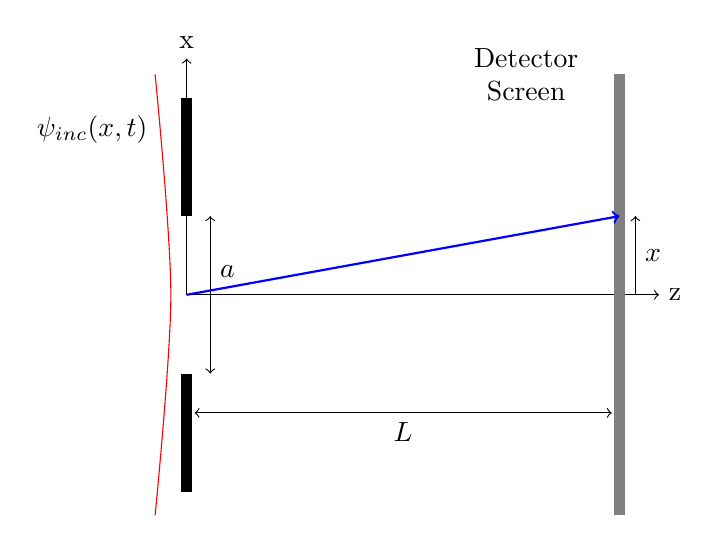
\begin{tikzpicture}

\draw[->](0,0) -- (6,0) node[right]{z};
\draw[->](0,0) -- (0,3) node[above]{x};

\draw[line width=4pt,black!50](5.5,-2.8) -- (5.5,2.8) node[left,black,text width=2cm, align=center]{Detector Screen};

\draw[line width=4pt](0,1) -- (0,2.5);
\draw[line width=4pt](0,-1) -- (0,-2.5);

\draw [red] plot [smooth] coordinates {(-.4,-2.8) (-.2,0) (-.4,2.8)} node[above,black,shift={(-.8,-1)}]{$\psi_\rmt{inc}(x,t)$};

\draw[<->] (.3,-1) -- (.3,1) node[midway,right,black,shift={(0,.3)}] {$a$};

\draw[<->] (.1,-1.5) -- (5.4,-1.5) node[midway,below]{$L$};

\draw[->,blue,thick](0,0) -- (5.5,1) node[midway,black,above]{};

\draw[->] (5.7,0) -- (5.7,1) node[midway,right]{$x$};

\end{tikzpicture}
\caption{Setup for a single slit diffraction experiment.  The MWM neutrons with wavefunction $\psi_{\rm inc}(x,t)$ are incident upon a slit of width $a$ that is centered on the $y$-axis in the $xy$-plane.  The neutrons are then observed to strike a screen a distance $L \gg a$ from the slit.}
\label{single slit setup}
\end{figure}

We model the experiment with the schematic shown in Fig.~\ref{single slit setup}.\footnote{The following derivation was heavily influenced by the treatment found in W. G\"{o}rlich, I. Hoffmann, T. Sch\"{u}rmann, arXiv:0812.4775v4 (2010).} The MWM neutrons with wavefunction $\psi_{\rm inc}(x,t)$ are incident upon a slit of width $a$ that is centered on the $y$-axis in the $xy$-plane.  The neutrons are then observed to strike a screen a distance $L \gg a$ from the slit.  For the Zeilinger experiment, $L = 5$~m, which is much larger than the slit width $a = 90$~$\mu$m.

Conceptually, what happens when the wavefunction reaches the slit is that only a piece of the wave passes through the slit. We'll model the slit as not changing the $z$ or $y$ properties of the wavefunction, but it chops the $x$ wavefunction so that after the slit it becomes:
\begin{marginfigure}
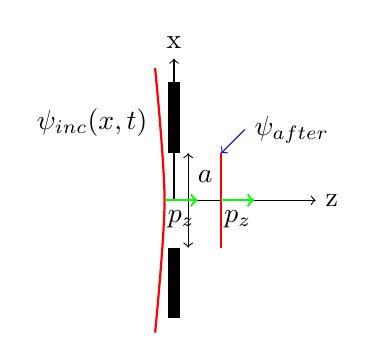
\begin{tikzpicture}[scale=0.6]

\draw[->](0,0) -- (3,0) node[right]{z};
\draw[->](0,0) -- (0,3) node[above]{x};


\draw[line width=4pt](0,1) -- (0,2.5);
\draw[line width=4pt](0,-1) -- (0,-2.5);

\draw [red,thick] plot [smooth] coordinates {(-.4,-2.8) (-.2,0) (-.4,2.8)} node[above,black,shift={(-.8,-1)}]{$\psi_\rmt{inc}(x,t)$};

\draw[red,thick] (1,-1) -- (1,1);
\draw[blue,->] (1.5,1.5) node[right,black]{$\psi_\rmt{after}$} -- (1,1);

\draw[<->] (.3,-1) -- (.3,1) node[midway,right,black,shift={(0,.3)}] {$a$};

\draw[->,thick,green] (-.2,0) -- (.5,0) node[midway,below,black]{$p_z$};

\draw[->,thick,green] (1,0) -- (1.7,0) node[midway,below,black]{$p_z$};

\end{tikzpicture}
\end{marginfigure}
%
\beq
\psi_\rmt{after}(x,0) = \begin{cases}\displaystyle \frac{1}{\sqrt{a}} & \displaystyle\abs{x}\leq \frac{a}{2}\\
0 &\displaystyle \abs{x}> \frac{a}{2}
\end{cases}
\eeq
where the $1/\sqrt{a}$ is the normalization constant for $\psi_\rmt{after}$ and we've set $t=0$ at the moment the wavefunction reaches the slit. To see what happens to the neutrons in the MWM, we need to know the momentum distribution. So we use Eq.~(\ref{eq:ftxtop}) to get the momentum wavefunction:
\bas
\phi(p_x)= &  \frac{1}{\sqrt{2\pi\hbar}}\int\displaylimits_{-\infty}^{\infty}\E{-\I \frac{p_x}{\hbar} x} \psi(x) dx \\
= &\frac{1}{\sqrt{2\pi\hbar a}}\frac{\E{\I p_x a/(2\hbar)}-\E{-\I p_x a/(2\hbar)}}{\I p_x/\hbar}\\
= & \sqrt{\frac{a}{2\pi\hbar}}\frac{\sin(p_x a/(2\hbar))}{p_x a/(2\hbar)}.
\eas
The momentum wavefunction probability density is thus 
\beq
\Pd(p_x) =  \frac{a}{2\pi\hbar}\left[\frac{\sin(p_x a/(2\hbar))}{p_x a/(2\hbar)}\right]^2.
\eeq
\begin{marginfigure}[-2cm]
\begin{tikzpicture}[scale=0.6]
\draw[->,thick] (-3,0) -- (3,0) node[right]{$p_x$};
\draw[->,thick] (0,-.2) -- (0,3) node[right]{$\Pd(p_x)$};

\begin{sagesilent}
x=var('x')
t = var('t')
x_coords = [t for t in srange(-3.0,3.0,.05)]
y_coords = [2.5*(sin(3*t))^2/(3*t)^2 for t in srange(-3.0,3.0,.05)]
output = ""
for i in range(0,len(x_coords)-1):
    output += r"\draw[blue, thick] (%f cm ,%f cm)--(%f cm ,%f cm);"%(x_coords[i],y_coords[i],x_coords[i+1],y_coords[i+1])
\end{sagesilent}

\sagestr{output}
\end{tikzpicture}
\end{marginfigure}

We now relate the momentum at the slit to the probability of the neutron reaching a particular position $x$ on the screen. A neutron with momentum $p_x$ at the slit will reach the screen at time $t=m L/p_z$ and will arrive at point
\beq
x = \frac{p_x}{m} t = \frac{p_x L}{p_z}.
\eeq
In order for the neutron to be detected on the screen in the range $x$ to $x+dx$, it must have momentum in the range $p_x$ to $p_x + dp_x$. So
\beq
dp_x = \frac{p_z}{L} dx
\eeq
Therefore, the probability of detecting the neutron in the region $dx$ is (written using the $z$-direction momentum scale $k_z = p_z/\hbar$)\arnote{Fill in the missing steps and substitutions.}\beq
\Pd(x) dx = \Pd(p_x)dp_x = \frac{k_z a}{2\pi L} \left[\frac{\sin(k_z a x /(2L))}{k_z a x /(2L)}\right]^2 dx.
\eeq
 This is very similar to the intensity pattern expected for single-slit diffraction for ElMaWs (Fig.~\ref{single slit light}). This reinforces the similarities we saw between our MWM and the ElMaW model. \marginnote{In particular we have the relationship between the probability density in the MWM and the intensity of ElMaWs:
\beq\Pd(x)\;\leftrightarrow\;I(x).\eeq}
\begin{figure}
\begin{center}
\includegraphics[width=0.8\textwidth]{SingleSlitLight}
\caption[][3cm]{Single slit diffraction intensity graph and photograph of actual pattern for light. [Taken from {\tt http://en.wikipedia.org/ wiki/Diffraction}] }
\label{single slit light}
\end{center}
\end{figure}
%

\section{Diffraction with Gratings}

We extend our MWM from diffraction by single slits discussed in the previous section to multiple slits.  The resulting measurement probability mimics what would be found in the optical case.  For $N$ slits of width $a$ with center-to-center separation $d$, the intensity on a screen a distance $L \gg a,d$ is\footnote{G. R. Fowles, {\em Introduction to Modern Optics}, 2nd ed. (Dover, New York, 1989), p.123.}
%
\beq
\Pd(x) = \Pd_{0}\,\left(\frac{\sin(k_z a x /(2L))}{k_z a x /(2L)}\right)^2 \left[\frac{\sin\left(\frac{N k_z d x}{2L}\right)}{N\sin\left(\frac{k_z d x}{2L}\right)}\right]^{2},
\label{N I x}
\eeq
%
where $\Pd_{0}$ is the probability density at $x = 0$.  Graphs of the ElMaW intensity $I(x)$ for several different values of $N$ are shown in Fig.~\ref{N slit graphs} where we see that increasing the number of slits narrows the interference maxima without changing their location.  The single slit diffraction pattern forms an envelope for the overall pattern.
%
\begin{figure}
\begin{center}
\includegraphics[width=0.8\textwidth]{NSlitgraphs}
\caption{Graphs of the $N$-slit intensity pattern obtained from Eq.~(\ref{N I x}) with slit separation $d = 3a$ ($a$ = slit width) for $N = 2$ and $20$ illustrating the narrowing of constructive peaks as $N$ increases.}
\label{N slit graphs}
\end{center}
\end{figure}
%
%

\begin{exercise}
Derive Eq.~(\ref{N I x}). You can look it up in a book and use that as a template if you need to. Verify that $\Pd(x = 0) = \Pd_{0}$  and that Eq.~(\ref{N I x}) reduces to the single slit result for $N = 1$.
\end{exercise}

%


The first demonstration of atomic beam interference with a nanofabricated diffraction grating was conducted by Keith, et al.  who diffracted a collimated beam of sodium atoms with a grating with $d = 0.2$~$\mu$m formed from a gold membrane.\footnote{D. W. Keith, et al., Phys. Rev. Lett. {\bf 61}, 1580 (1988).}  A schematic of a matter wave diffraction grating experiment is shown to the right, and data from the Keith experiment is shown below the schematic. 
Many other groups refined this technique, sharpening the maxima to levels more comparable to what has been achieved at the optical level (e.g., see  A. D. Cronin, J. Schmiedmayer, and D. E. Pritchard {\bf 81}, 1051 (2009)).
%
\begin{marginfigure}
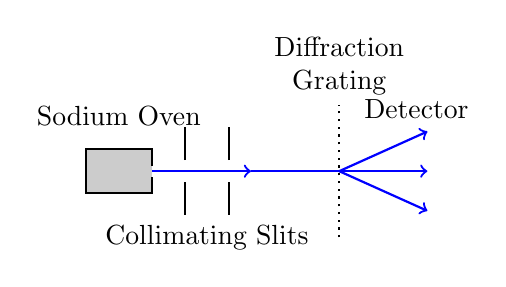
\begin{tikzpicture}[scale=0.28]
\fill[black!20] (-1.5,-1) rectangle +(3,2);
\draw[thick] (1.5,.25) -- (1.5,1) -- (-1.5,1) -- (-1.5,-1) -- (1.5,-1) -- (1.5,-.25);
\node at (0,2.5){Sodium Oven};
\draw[->,thick,blue] (1.5,0) -- (6,0);
\draw[thick,blue] (6,0) -- (10,0);
\draw[dotted,thick](10,-3) -- (10,3) node[above,text width=2cm,align=center]{Diffraction Grating};

\draw[thick] (3,.5)-- (3,2);
\draw[thick] (3,-.5)-- (3,-2);

\draw[thick] (5,.5)-- (5,2);
\draw[thick] (5,-.5)-- (5,-2);

\node at (4,-3){Collimating Slits};

\draw[->,thick,blue](10,0) -- (14,1.8);
\draw[->,thick,blue](10,0) -- (14,0);
\draw[->,thick,blue](10,0) -- (14,-1.8);

\node at (13.5,2.8){Detector};
\detector{1}{14}{1.8}{0}

\end{tikzpicture}
\includegraphics[width=0.95\textwidth]{Keith-Diffraction}
\caption{The top graph (a) shows the atomic intensity pattern without the grating, while the bottom graph (b) shows the central maximum and two first-order constructive peaks when the grating is put in place.}
\end{marginfigure}


All of this work was done with diffraction gratings made of materials, but it turns out this is not the only way to make a grating.  Light exerts forces on atoms and a diffraction grating can be made with a standing optical wave. Furthermore, early work on diffraction gratings (\ie Bragg scattering) used electrons scattered from crystal lattices. All of these experiments can be modeled using MWM interference.

\begin{exercise}
Determine and plot the diffraction intensity pattern for the Keith grating experiment which
used sodium atoms traveling about 1000 m/s. The grating period was 0.2 $\mu$m, and the detector was placed about 1.5 m from the grating. From the photograph in the paper, the slit width appears to be about 1/3rd the slit spacing.
\end{exercise}

\section{Three-Grating Interferometers}

Diffraction gratings are particularly good at producing clear interference patterns demonstrating the wave properties of matter.   A wave passing through a grating could have come from any one of a significant number of slits, which produces very sharp constructive interference fringes. The fact that the fringes produced by gratings are so sharp implies a property that makes them very useful for applications: they coherently split a single beam into multiple beams.  Using multiple gratings allows one to coherently split, reflect, and recombine beams, forming an interferometer. A schematic of a  3-grating interferometer  is shown in Fig.~\ref{3-grating interferometer}.
\begin{figure}
\centering
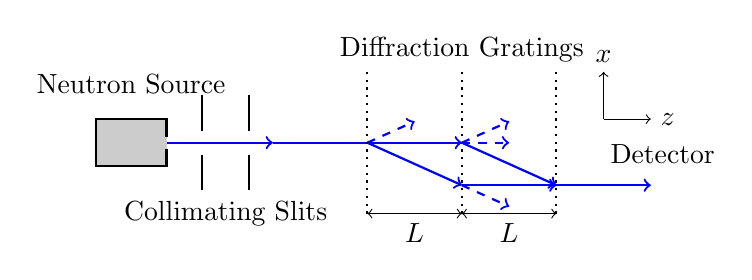
\begin{tikzpicture}[scale=0.3]
\fill[black!20] (-1.5,-1) rectangle +(3,2);
\draw[thick] (1.5,.25) -- (1.5,1) -- (-1.5,1) -- (-1.5,-1) -- (1.5,-1) -- (1.5,-.25);
\node at (0,2.5){Neutron Source};
\draw[->,thick,blue] (1.5,0) -- (6,0);
\draw[thick,blue] (6,0) -- (10,0);


\draw[thick] (3,.5)-- (3,2);
\draw[thick] (3,-.5)-- (3,-2);

\draw[thick] (5,.5)-- (5,2);
\draw[thick] (5,-.5)-- (5,-2);

\node at (4,-3){Collimating Slits};

\draw[->,thick,blue,dashed](10,0) -- (12,0.9);
\draw[->,thick,blue](10,0) -- (14,0);
\draw[->,thick,blue](10,0) -- (14,-1.8);

\draw[dotted,thick](10,-3) -- (10,3);

\draw[dotted,thick](14,-3) -- (14,3) node[above,align=center]{Diffraction Gratings};

\draw[dotted,thick](18,-3) -- (18,3);

\draw[->,thick,blue](14,0) -- (18,-1.8);
\draw[->,thick,blue,dashed](14,0) -- (16,0);
\draw[->,thick,blue,dashed](14,0) -- (16,0.9);
\draw[->,thick,blue](14,-1.8) -- (18,-1.8);
\draw[->,thick,blue,dashed](14,-1.8) -- (16,-2.7);

\draw[->,thick,blue](18,-1.8) -- (22,-1.8);
\node at (22.5,-0.5){Detector};
\detector{1}{22.5}{-1.8}{0}

\draw[->](20,1) -- (22,1) node[right]{$z$};
\draw[->](20,1) -- (20,3) node[above]{$x$};

\draw[<->](10,-3) -- (14,-3)node[midway,below]{$L$};
\draw[<->](14,-3) -- (18,-3)node[midway,below]{$L$};
\end{tikzpicture}
\caption[][-1cm]{A schematic of a 3-grating interferometer.  The dark lines indicate the primary beams of particles to be used, while the dashed lines represent some of the secondary beams not used in the experiment.}
\label{3-grating interferometer}
\end{figure}
Three-grating interferometers have been built for atomic beams using material and optical gratings.\footnote{A. D. Cronin, J. Schmiedmayer, and D. E. Pritchard {\bf 81}, 1051 (2009).} and for neutrons using perfect silicon crystal interferometers (Fig.~\ref{neutron interferometer}).  Matter interferometers have a wide variety of applications in addition to probing fundamental physics.  Since atoms have internal degrees of freedom, there are many more variations of experiments one can do in matter interferometry than with light, and with greater position.  Better atomic clocks and accelerometers are just two examples.
%
 \begin{marginfigure}
\begin{center}
\includegraphics[width=.8\textwidth]{NeutronInterferometer}
\caption{A perfect silicon crystal neutron interferometer.  [Taken from K. C. Kittrell, B. E. Allman, and S. A. Werner, Phys. Rev. A. {\bf 56}, 1767 (1997).]}
\label{neutron interferometer}
\end{center}
\end{marginfigure}
%

\section{Path Integral Model}
\label{sec:pathIntegral}
We return to the Schr\"{o}dinger Equation and the time evolution of our one-dimensional continuous quantum state. Given that we know the state of the freely evolving system at time $t_1$: $\ket{\Psi(x_1,t_1)}\equiv\ket{x_1}$, what is the state of the system at some later time, $t_2$, $\ket{\Psi(x_2,t_2)}\equiv\ket{x_2}$? Since our Hamiltonian ($\hat{H} = \hat{P}_x^2/(2m)$) is time-independent, we can informally solve the  Schr\"{o}dinger Equation, Eq.~(\ref{eq:sch}):\marginnote{We saw in Section \ref{sec:thermalstates} how to work with an operator in the exponent. We use the \ref{tool:sch}.}
\bas
\I \hbar \frac {d}{dt}\ket{\Psi} = &  \hat{H}\ket{\Psi} \\
\downarrow\\
\ket{\Psi(t)} = &\E{-\I \frac{\hat{H}}{\hbar} t}\ket{\Psi(0)}
\eas
So now we can find the evolution starting with the specific state $\ket{x_1}$ and get
\beq
\ket{\Psi(x_2,t_2)} = \E{-\I \frac{\hat{H}}{\hbar} (t_2 - t_1)}\ket{x_1}
\eeq
for total energy $H = p_x^2/(2m)$. We'll first call the time difference $t_2 - t_1 \equiv \Delta t$. We define the amplitude $C(x_1,t_1;x_2,t_2)$ (or just $C_{1,2}$) as the inner product of $\avg{x_2|\Psi(x_2,t_2)}$:
\beq
C_{1,2} \equiv \bra{x_2} \E{-\I \frac{\hat{H}}{\hbar} \Delta t}\ket{x_1}.
\eeq
If we now cut the time interval in half and insert a spanning basis in $x$, we get:
\bas
C_{1,2} =& \bra{x_2} \E{-\I \frac{\hat{H}}{\hbar} \Delta t/2}\E{-\I \frac{\hat{H}}{\hbar} \Delta t/2}\ket{x_1} \\
=&\int\displaylimits_{-\infty}^{\infty}\bra{x_2} \E{-\I \frac{\hat{H}}{\hbar} \Delta t/2}\ket{x}\bra{x}\E{-\I \frac{\hat{H}}{\hbar} \Delta t/2}\ket{x_1}dx.\label{eq:pathintegral}
\eas
The meaning of this is the Feynman Path Integral: to find the amplitude of a state going from $x_1$ to $x_2$, we add up the amplitudes of the state moving through all possible intermediate states. If we are moving along a single path, or several discrete paths, we just need to add up the phases $C_{a,b}$ for each step along the path. This is equivalent to the interference model we used for the CEWAM in Section \ref{sec:CEWAM}.

\section{Simple Mach-Zehnder Matter Interferometer}

To understand better how a matter interferometer works, we're going to step away from the 3-grating interferometer and instead analyze a simpler matter analog of an optical Mach-Zehnder (M-Z) interferometer.\footnote{The treatment in this section was inspired by J. S. Townsend, {\em Quantum Physics}, (University Science Books, Sausalito, CA, 2010), Chapter 1.}  This will lead to essentially the same results as the 3-grating interferometer without having to delve more deeply into the details of the multiple beams produced by a grating. We start with the setup for  a typical M-Z interferometer (Fig.~\ref{M-Z setup}).  
%
\begin{figure}
\centering
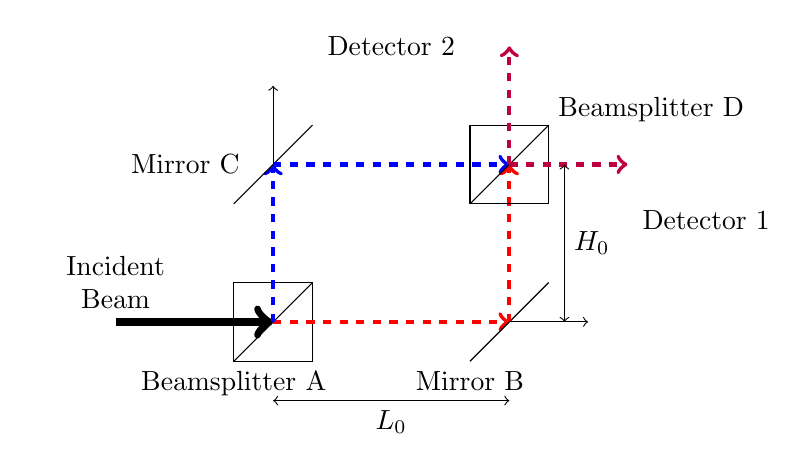
\begin{tikzpicture}
%beamsplitter 1
\draw (-0.5,-.5)node[below]{Beamsplitter A} rectangle +(1,1) ;
\draw (-.5,-.5) -- (.5,.5);


\draw[black,->,line width=3pt](-2,0)--(0,0) node[midway, above,shift=({-1cm,0}),text width=2cm,align=center]{Incident Beam};

%red beam
\draw[red,->,dashed,line width=1.5pt](0,0)--(3,0);
\draw (2.5,-.5)node[below]{Mirror B} -- (3.5,.5);
\draw[red,->,dashed,line width=1.5pt](3,0)--(3,2);
\draw[black,->](3,0) -- (4,0);

%blue beam
\draw[blue,->,dashed,line width=1.5pt](0,0)--(0,2);
\draw (-.5,1.5) node[left,shift={(0.2,.5)}]{Mirror C}-- (.5,2.5) ;
\draw[blue,->,dashed,line width=1.5pt](0,2)--(3,2);
\draw[->](0,2) -- (0,3);

\draw (2.5,1.5) rectangle +(1,1)node[above,right,shift={(0,.2)}]{Beamsplitter D} ;
\draw (2.5,1.5) -- (3.5,2.5);

%output beams
\draw[purple,->,dashed,line width=1.5pt](3,2) -- (3,3.5);
\draw[purple,->,dashed,line width=1.5pt](3,2) -- (4.5,2);

\detector{1}{4.5}{2}{0}
\node at (5.5,1.3) {Detector 1};

\detector{1}{3}{3.5}{90}
\node at (1.5,3.5) {Detector 2};

\draw[<->] (0,-1) -- (3,-1) node[midway,below]{$L_0$};

\draw[<->] (3.7,0) -- (3.7,2) node[midway,right]{$H_0$};

\end{tikzpicture}
\caption[][1cm]{Setup for a typical  Mach-Zehnder interferometer.}
\label{M-Z setup}
\end{figure}
%

We model the incident collimated atomic (or other quantum object) beam has having a well-defined initial momentum $p_{0} = \hbar k_{0}$. The beam passes through 50:50 beamsplitter A, which splits the beam equally into two new beams, one which is transmitted directly toward mirror B, while the other beam is reflected toward mirror C.  The mirrors then reflect the beams  toward the second 50:50 beamsplitter D, from which the beams may be transmitted to either of two detectors \#1 and \#2.  By comparing Fig.~\ref{M-Z setup} with Fig.~\ref{3-grating interferometer}, we see that in a 3-grating interferometer, the first grating plays the role of beamsplitter A, the second grating plays the role of the two mirrors B and C, and the third grating acts as beamsplitter D.  

\subsection{Wavefunction Propagation}

Because our model has the incident beam with a well-defined wave number $k_{0}$, this implies that the wave functions are approximately
%
\begin{equation}
\Psi(s,t) =  A\E{ik_{0}s}\E{-i\omega_{0}t},
\end{equation}
%
where $\omega_{0} = p_{0}^{2}/(2m\hbar)$ and $s$ is the position variable along the direction of motion.  We model the beam's interaction with the beam splitters and mirrors as elastic collisions so that the kinetic energy (and thus, $\omega_{0}$) does not change.  Therefore all wave functions will have the same overall factor $\E{-i\omega_{0}t},$ which can be then ignored.  Thus, we model the free propagation of the wavefunction inside the interferometer using the time-independent wave function
%
\begin{equation}
\psi(s) =  \E{ik_{0}s},
\end{equation}
%
where $s$ is the distance traveled by the beam and we've set the normalization constant $A = 1$ for later convenience.

\subsection{Beamsplitters}

What happens when the matter wave reaches a beamsplitter?  For convenience, we are going to model the beamsplitter as a 50:50 beamsplitter, which means that there is a 50\% chance that the object will be either transmitted or reflected.  We consider the complex amplitudes for transmission and reflection, ${\cal T}_{\rm bs}$ and ${\cal R}_{\rm bs}$, respectively, such that
%
\bas
\rmt{Probability of transmission} & = |{\cal T}_{\rm bs}|^{2} = \frac{1}{2}, \\
\rmt{Probability of reflection} & =  |{\cal R}_{\rm bs}|^{2} = \frac{1}{2}.
\eas
%
We saw in Section \ref{sec:EMbeamsplitter} that there was a $90^\circ$ phase shift on reflection from the ElMaW beamsplitter.  Experiments show that this is also the case in the MWM. So we model the transmission and reflection amplitudes as
%
\bas
{\cal T}_{\rm bs} = & \frac{1}{\stwo}, \\
{\cal R}_{\rm bs} = & \frac{\I}{\stwo}.
\eas

\subsection{Mirrors}

We model the mirrors as ideal mirrors that reflect 100\% of the beam. Again, there is a phase shift on reflection, so we model the reflection coefficient for a mirror as
%
\beq
{\cal R}_{\rm m} = -1.
\eeq
%
We now have everything we need to model the motion of a matter wave through the M-Z interferometer.

\subsection{Detection Probability}
\label{MZ detection probability section}
We now make use of the path integral model from Section \ref{sec:pathIntegral}: to find the probability amplitude that the beam reaches detector \#1, we multiply all the amplitudes of the stages along each path. Our model from Fig.~\ref{M-Z setup}, implies that there are two different paths from Beamplitter A to detector \#1:  
%
\begin{center}
\begin{tabular}{ll}
Path ABD: & A $\rightarrow$ B $\rightarrow$ D $\rightarrow$ detector \#1, \\
Path ACD: & A $\rightarrow$ C $\rightarrow$ D $\rightarrow$ detector \#1. 
\end{tabular}
\end{center}
%
In the MWM, total quantum probability of reaching detector \#1 is obtained by (modulus) squaring the sum of the quantum amplitudes of reaching detector \#1 for  each path.  

\subsection{Path ABD}

We begin by modeling the input amplitude of the wave on beam splitter A as
%
\beq
\psi_\rmt{inc} = \E{ik_{0}s_{0}}
\eeq
%
where $s_{0}$ is a constant which could be the distance from the beam source. The aplitudes for this path are
\begin{enumerate}
\item{\bf Incident Amplitude:} $\psi_\rmt{inc}$
\item{\bf Transmission by Beamsplitter A:} $\psi_{A} = {\cal T}_{\rm bs}$
\item{\bf Propagation from Beamsplitter A to Mirror B:} $\psi_{A \rightarrow B} = \E{ik_{0}s_{A \rightarrow B}} = \E{ik_{0}L_{0}}$
\item{\bf Reflection by Mirror B:} $\psi_{B} = {\cal R}_{\rm m}$
\item{\bf Propagation from Mirror B  to Beamsplitter D:} $\psi_{B \rightarrow D} = \E{ik_{0}s_{B \rightarrow D}} = \E{\I k_{0}H_{0}}$
\item{\bf Reflection  by Beamsplitter D into Detector \#1:} $\psi_{D} = {\cal R}_{\rm bs}$
\end{enumerate}
%
Putting all this together gives the total quantum amplitude of reaching detector \#1 via path ABD:\arnote{Make sure you can fill in the missing steps.}
%
\bas
\psi_{ABD} &=   \psi_{\rm inc} \psi_{A} \psi_{A \rightarrow B} \psi_{B}  \psi_{B \rightarrow D}\psi_{D}, \\
	&=  \E{\I k_{0}s_{0}} {\cal T}_{\rm bs} \E{\I k_{0}L_{0}} {\cal R}_{\rm m}   \E{\I k_{0}H_{0}}   {\cal R}_{\rm bs}, \\
%	&=  \E{\I k_{0}s_{0}}\left( \frac{1}{\sqrt{2}}\right)\left(\E{\I k_{0}L_{0}} \right)\left(-1\right)\left(\E{\I k_{0}H_{0}}\right)\left(\frac{i}{\sqrt{2}}\right), \nonumber \\
	& =  -\I\frac{1}{2}\E{\I k_{0}s_{0}}\E{\I k_{0}(L_{0} + H_{0})}.
	\label{psi ABD}
\eas

\subsection{Path ACD}

Similarly, the   amplitude for  path ACD comes from the steps
%
\begin{enumerate}
\item{\bf Incident Amplitude:} $\psi_{\rm inc}$
\item{\bf Reflection by Beamsplitter A:} $\psi_{A} = {\cal R}_{\rm bs}$
\item{\bf Propagation from Beamsplitter A to Mirror C:} $\psi_{A \rightarrow C} = \E{\I k_{0}s_{A \rightarrow C}} = \E{\I k_{0}H_{0}}$
\item{\bf Reflection by Mirror C} $\psi_{C} = {\cal R}_{\rm m}$
\item{\bf Propagation from Mirror C  to Beamsplitter D:} $\psi_{C \rightarrow D} = \E{\I k_{0}s_{C \rightarrow D}} = \E{\I k_{0}L_{0}}$
\item{\bf Transmission  by Beamsplitter D into Detector \#1:} $\psi_{D} = {\cal T}_{\rm bs}$
\end{enumerate}
%
Putting all this together gives the total quantum amplitude of reaching detector \#1 via path ACD:\arnote{Again, there are steps missing - make sure you've got them.}
%
\bas
\psi_{ACD} &=   \psi_{\rm inc} \psi_{A} \psi_{A \rightarrow C} \psi_{C}  \psi_{C \rightarrow D}\psi_{D}, \\
	&=  \E{\I k_{0}s_{0}} {\cal R}_{\rm bs} \E{\I k_{0}H_{0}} {\cal R}_{\rm m}   \E{\I k_{0}L_{0}}   {\cal T}_{\rm bs}, \\
%	&=  \E{\I k_{0}s_{0}}\left( \frac{i}{\sqrt{2}}\right)\left(\E{\I k_{0}H_{0}} \right)\left(-1\right)\left(\E{\I k_{0}L_{0}}\right)\left(\frac{1}{\sqrt{2}}\right), \nonumber \\
	& =  -\I\frac{1}{2}\E{\I k_{0}s_{0}}\E{\I k_{0}(L_{0} + H_{0})}.
	\label{psi ACD}
\eas
%
Notice that the probability amplitudes for each path are the same in this case: $\psi_{ABD} = \psi_{ACD}$.

\subsection{Probability Density for Reaching Detector \#1}

The total probability density for reaching detector \#1, $P_{1}$ is then obtained by modulus squaring the sum of the two amplitudes: \arnote{More missing steps here - work them out in your notes.}
%
\bas
\Pd_{1} & =  \left|\psi_{ABD}  + \psi_{ACD} \right|^{2} \\
	& =  \left|-\I\frac{1}{2}\E{\I k_{0}s_{0}}\E{\I k_{0}(L_{0} + H_{0})} - \I\frac{1}{2}\E{\I k_{0}s_{0}}\E{\I k_{0}(L_{0} + H_{0})}\right|^{2} =1.
%	& =  \left|\frac{1}{2} + \frac{1}{2}\right|^{2}\left|-i\E{\I k_{0}s_{0}}\E{\I k_{0}(L_{0} + H_{0})}\right|^{2}=1. \\
\eas
%
Thus, there is a 100\% chance the particle will reach detector \#1, while the probability density of reaching detector \#2 with this setup is zero.

What happens if we block path ABD?  Then the matter wave can only reach detector \#1 via path ACD,  and so the probability density of detection by \#1 is
%
\bas
\Pd_{1} & = \left|\psi_{ACD}\right|^{2} \nonumber \\
	& = \left|-i\frac{1}{2}\E{\I k_{0}s_{0}}\E{\I k_{0}(L_{0} + H_{0})} \right|^{2}\nonumber \\
	& =  \left|\frac{1}{2}\right|^{2} =\frac{1}{4}.\\
	\eas
%
The probability density for detection by detector \#2 for the blocked path case is also $\Pd_{2} = 1/4$. \arnote{Work this one out.}  Notice that $\Pd_{1} + \Pd_{2} = 1/2$ for the blocked path case because beamsplitter A will send half the beam into the blocked path so that part of the beam never reaches the detectors.  

\begin{exercise}
Show that the probability density that the particle reaches detector \#2 is zero.
\end{exercise}

\begin{exercise}
\label{ex:modmz}
Consider the M-Z experiment setup shown in Figure \ref{fig:modmzsetup} that is just like the previous one except a phase shifter has been inserted in the path C $\rightarrow$ D.  The phase shifter  multiplies the propagation amplitude $e^{ik_{0}s}$ for particles traveling this path by a phase factor $e^{i\varphi}$, where we can control the value of the angle $\varphi$.  [For light, this can be accomplished by inserting a plate of glass.]  Nearly all interferometry experiments involve doing something to one path and not to the other, and then looking for the effects (a phase difference) this causes in the detection probability densities.  Such phase differences are easily detectable so they form the basis of some of the most sensitive experiments in physics.
%
\begin{figure}
\centering
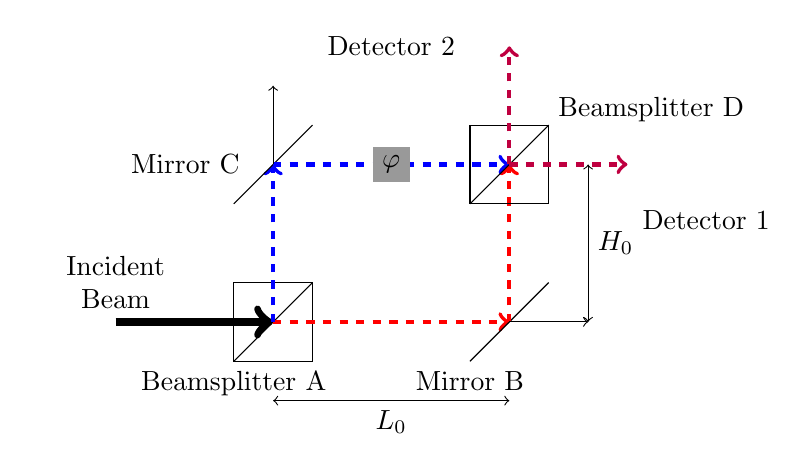
\begin{tikzpicture}
%beamsplitter 1
\draw (-0.5,-.5)node[below]{Beamsplitter A} rectangle +(1,1) ;
\draw (-.5,-.5) -- (.5,.5);


\draw[black,->,line width=3pt](-2,0)--(0,0) node[midway, above,shift=({-1cm,0}),text width=2cm,align=center]{Incident Beam};

%red beam
\draw[red,->,dashed,line width=1.5pt](0,0)--(3,0);
\draw (2.5,-.5)node[below]{Mirror B} -- (3.5,.5);
\draw[red,->,dashed,line width=1.5pt](3,0)--(3,2);
\draw[black,->](3,0) -- (4,0);

%blue beam
\draw[blue,->,dashed,line width=1.5pt](0,0)--(0,2);
\draw (-.5,1.5) node[left,shift={(0.2,.5)}]{Mirror C}-- (.5,2.5) ;
\draw[blue,->,dashed,line width=1.5pt](0,2)--(3,2);
\draw[->](0,2) -- (0,3);

\node[rectangle,fill=black!40] at (1.5,2){$\varphi$};


\draw (2.5,1.5) rectangle +(1,1)node[above,right,shift={(0,.2)}]{Beamsplitter D} ;
\draw (2.5,1.5) -- (3.5,2.5);

%output beams
\draw[purple,->,dashed,line width=1.5pt](3,2) -- (3,3.5);
\draw[purple,->,dashed,line width=1.5pt](3,2) -- (4.5,2);

\detector{1}{4.5}{2}{0}
\node at (5.5,1.3) {Detector 1};

\detector{1}{3}{3.5}{90}
\node at (1.5,3.5) {Detector 2};

\draw[<->] (0,-1) -- (3,-1) node[midway,below]{$L_0$};

\draw[<->] (4,0) -- (4,2) node[midway,right]{$H_0$};

\end{tikzpicture}
\caption[][2cm]{Figure for Exercise \ref{ex:modmz}.}
\label{fig:modmzsetup}
\end{figure}

\begin{enumerate}
\item  Calculate the probability density that the beam will be detected by each detector, $\Pd_{1}(\varphi)$ and $\Pd_{2}(\varphi)$.  Show that $\Pd_{1}(\varphi) + \Pd_{2}(\varphi) = 1$, and that they reduce to the expected values when $\varphi = 0$.
\item  Plot $\Pd_{1}(\varphi)$ and $\Pd_{2}(\varphi)$ on the same graph as functions of $\varphi$. 
\end{enumerate}


\end{exercise}


%---------------------------------------

\chapter{Wave Packets}

As we've been working with the free propagation of wavefunctions in the MWM, we've ignored a pretty important piece of the model. The wavefunction, as written in Eq.~(\ref{eq:tdsefreesol}) is not normalizable:
\bas
\psi(x,t)& = A \E{\I (k x -\omega t)}\\
&\downarrow\nonumber\\
\intii \abs{\psi(x,t)}^2 dx &= \infty.
\eas
However, there is a modification to this model that makes it work. These wavefunctions actually represent an infinite number of possible solutions; we can add up solutions to make a {\em wave   packet} that is normalizable. We saw this in Eq.~(\ref{eq:tdsefreesolint})
\beq
\psi(x,t) = \sqrt{\frac{\hbar}{2\pi}}  \intii\phi(\hbar k,0) \E{\I(kx-\omega(k) t)}dk
\eeq
where the initial momentum wavefunctions $\phi(\hbar k,0)$ also need to be normalizable. The good news is that this gives us the possibility for making normalizable MWM wave  packets. The bad news is that there are only a few functions that make these integrals analytically doable. We'll focus on one of them: the Gaussian wave  packet. \marginnote[-1cm]{Another type of wave  packet is the function $\sqrt{\frac{\alpha}{2}}\rmt{sech}(\alpha(k-k_0)).$}

\section{Gaussian wave  packets}


\subsection{Modeling a Classical Particle}

One of the aspects of this model that we are interested in is the ability to model a classical particle. We would like to be able to make repeated measurements of our MWM wavefunction and get a set of results similar to a classical Gaussian measurement probability distribution function. We can then connect our classical measurement uncertainties with the quantum measurement uncertainties. We call this the {\em Gaussian Wave Packet Particle Model}. Furthermore, it will give us the quantum state with the smallest $\Delta X\Delta P_{x}$ permitted by the Heisenberg uncertainty principle.

\subsection{Properties of a Gaussian Probability Distribution}
\begin{marginfigure}

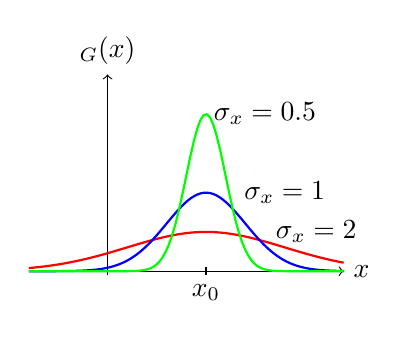
\begin{tikzpicture}[scale=0.5]
\draw[->](-2,0) -- (6,0)node[right]{$x$};
\draw[->](0,-0.1) -- (0,5)node[above]{$\Pd_G(x)$};
\draw[domain=-2:6,samples=100,thick,red] plot({\x},{5/(2*sqrt(2*pi))*exp(-(\x-2.5)^2/(2*2^2)});
\draw[domain=-2:6,samples=100,thick,blue] plot({\x},{5/(1*sqrt(2*pi))*exp(-(\x-2.5)^2/(2*1^2)});
\draw[domain=-2:6,samples=100,thick,green] plot({\x},{5/(0.5*sqrt(2*pi))*exp(-(\x-2.5)^2/(2*0.5^2)});
\node at (5.3,1) {$\sigma_x = 2$};
\node at (4.5,2) {$\sigma_x = 1$};
\node at (4,4) {$\sigma_x = 0.5$};
\draw (2.5,0.1) -- (2.5,-0.1) node[below]{$x_0$};
\end{tikzpicture}
\caption{Graphs of $\Pd_{G}(x)$ with average $x_{0}$ and $\sigma_{x} = 0.5, 1$ and 2.}
\label{Gaussian P graphs}
\end{marginfigure}
We begin with a quick review of the properties of the Gaussian probabilities distribution ${\cal P}_{G}(x)$ which is given by
%
\beq
\Pd_{G}(x) = \frac{1}{\sigma_{x}\sqrt{2\pi}}\E{-(x - x_{0})^{2}/(2\sigma_{x}^{2})},
\label{Gaussian P}
\eeq
%
where $\sigma_{x}$ is the root-mean-square deviation of the distribution and $x_{0}$ is the average. As shown in Fig.~\ref{Gaussian P graphs}, $x_{0}$ denotes the location of the maximum value of $\Pd_{G}(x)$ while $\sigma_{x}$ characterizes the width of the curve. About 68\% of the total area under the curve lies within the range $x_{0}-\sigma_{x} \leq x \leq x_{0}+\sigma_{x}$. \arnote{The 68\% property is a good one for you to work out. Do the definite integral with these limits.}

\begin{exercise}
Use Eq.~(\ref{Gaussian P}) to show that
%
\bas
\avg{\hat{X}} & =  \intii \Pd_{G}(x)\,x \, dx = x_{0}, \\
\avg{\hat{X}^2} & =  \intii \Pd_{G}(x)\,x^2 \, dx = x_{0}^2 + \sigma_x^2,
\eas
%
and, therefore,
%
\beq
\Delta X = \sqrt{\avg{\hat{X}^2} -\avg{\hat{X}}^2} = \sigma_{x}.
\eeq
\end{exercise}


\subsection{Gaussian Wave Packet}

We now model a classical particle with a Gaussian  wave packet that characterizes the information about the particle's position.  Since a particle exists in three dimensions, we model the full 3-dimensional wave function $\Psi(x,y,z,t)$ as a product of wave functions in each dimension,\marginnote{We've talked about using multiple parameters to describe our quantum state. This is one place where we will do this explicitly. Since the three spatial dimensions are orthogonal, they can be treated independently, just like in classical mechanics.}
%
\begin{equation}
\Psi(x,y,z,t) = \Psi(x,t)\Psi(y,t)\Psi(z,t)
\end{equation}
%
so that we can focus on the model in the $x$-direction and then extend the results for the other two dimensions.

We begin by modeling the particle with a wave function $\psi_{G}(x,0)$ that characterizes a quantum particle at position $x_{0}$ at $t = 0$ with momentum $p_{x} = p_{0}$ and rms deviations $\sigma_{x}$ and $\sigma_{p} = \hbar/2\sigma_{x}$, respectively.  (To be consistent with the HUR, we  want $\sigma_{x}\sigma_{p} = \hbar/2$.) Since $\Pd(x) = \abs{\psi(x)}^{2}$, we try the wavefunction
%
\beq
 \psi_{G}(x,0) \stackrel{?}{=} \sqrt{\Pd_{G}(x)} =  \frac{1}{(2\pi\sigma_{x}^{2})^{1/4}}\E{-(x - x_{0})^{2}/(4\sigma_{x}^{2})}.
 \label{Psi G guess}
 \eeq
 %
 While this gives the desired position statistics, there's nothing that would give the particle momentum $p_{0}$.  In order to add the momentum information, we multiply Eq.~(\ref{Psi G guess}) by a phase factor $\E{\I\alpha}$ which does not affect the probability density.  A particle with definite momentum $p_{x} = p_{0}$ has a wave function $\psi_{p}(x) \propto \E{\I p_{0}x/\hbar}$.  So if we multiply Eq.~(\ref{Psi G guess}) by $\E{\I p_{0}x/\hbar}$ we get a model that has both sets of properties:\marginnote{We already saw this one in Exercise \ref{ex:firstgauss}.}
 %
\beq
 \psi_{G}(x,0) =  \frac{1}{(2\pi\sigma_{x}^{2})^{1/4}}\E{-(x - x_{0})^{2}/(4\sigma_{x}^{2})}\E{\I p_{0}x/\hbar}.
 \label{Psi G}
 \eeq
 %
This has the right statistical properties for the momentum as well. The momentum wave function is,  using the modified Fourier transform from Eq.~(\ref{eq:ftxtop}),\arnote{Fill in the missing steps here.}
\bas
 \phi_{G}(p_{x},0)  =&  \frac{1}{\sqrt{2\pi\hbar}}\intii \psi_{G}(x,0)\E{- \I p_{x}x/\hbar}dx \\
  = & \sqrt{\frac{2\sigma_{x}}{\hbar}}\left(\frac{1}{2\pi}\right)^{1/4}\E{-(p_{x}-p_{0})^{2}\sigma_{x}^{2}/\hbar^{2}}\E{\I (p_{0}-p_{x})x_{0}/\hbar}\label{eq:phigpx}.
\eas
The momentum probability density is then
%
\beq
\Pd_{G,p}(p_{x}) = \abs{\phi_{G}(p_{x},0)}^{2} 
		= \frac{2\sigma_{x}}{\hbar}\left(\frac{1}{2\pi}\right)^{1/2}\E{-(p_{x}-p_{0})^{2}(2\sigma_{x}^{2}/\hbar^{2})},
\label{P G p 1}
\eeq
%
where we've dropped the time dependence since we saw earlier that the momentum probability density of a free particle is independent of time.
If we define the momentum wave   packet spread as
%
\beq
\sigma_{p} \equiv \frac{\hbar}{2\sigma_{x}},
\eeq
%
then Eq.~(\ref{P G p 1}) becomes
%
\beq
\Pd_{G,p}(p_{x})  =  \frac{1}{\sigma_{p}\sqrt{2\pi}}\E{-(p_{x} - p_{0})^{2}/(2\sigma_{p}^{2})}.
 \label{P G p}
 \eeq
 % 
So our model now has a Gaussian position probability density with average position $x_{0}$ and rms deviation $\sigma_{x}$, and a Gaussian momentum probability density with average momentum $p_{x} = p_{0}$ and rms deviation $\sigma_{p} = \hbar/2\sigma_{x}$.  In addition, at $t = 0$, the Heisenberg uncertainty relationship is satisfied at the lowest possible (optimal) value,
 %
 \beq
 \Delta X\Delta P_{x} = \sigma_{x}\sigma_{p} = \sigma_{x} \left(\frac{\hbar}{2\sigma_{x}}\right) = \frac{\hbar}{2}.
 \label{Gaussian HUP}
 \eeq
 %
 The effect of Eq.~(\ref{Gaussian HUP}) is illustrated in Fig.~\ref{Gaussian XP graphs} where we see that a well-defined position (small $\sigma_{x}$) implies a less well-defined momentum (large $\sigma_{p}$).
 
\begin{exercise}
Use Eq.~(\ref{eq:phigpx}) to show that
%
\bas
\avg{\hat{P}_x} & =  p_{0}, \\
\avg{\hat{P}_x^2} & =  p_{0}^2 + \sigma_p^2,
\eas
%
and, therefore,
%
\begin{equation}
\Delta P_x = \sqrt{\avg{\hat{P}_x^2} -\avg{\hat{P}_x}^2} = \sigma_{p}.
\end{equation}
\end{exercise}
 
 \begin{marginfigure}

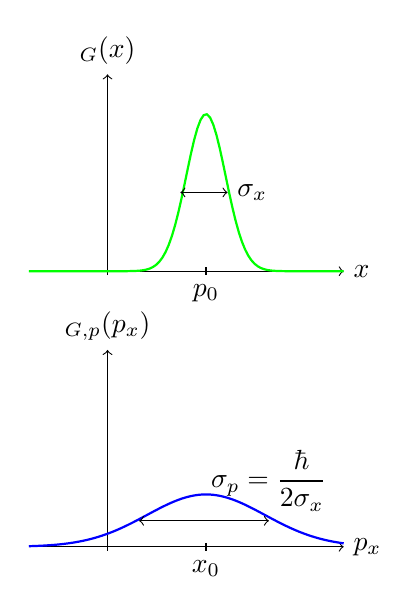
\begin{tikzpicture}[scale=0.5]
\draw[->](-2,0) -- (6,0)node[right]{$x$};
\draw[->](0,-0.1) -- (0,5)node[above]{$\Pd_G(x)$};
\draw[domain=-2:6,samples=100,thick,green] plot({\x},{5/(0.5*sqrt(2*pi))*exp(-(\x-2.5)^2/(2*0.5^2)});
\draw[<->] (1.85,2) -- (3.05,2) node[right] {$\sigma_x$};

\draw (2.5,0.1) -- (2.5,-0.1) node[below]{$p_{0}$};
\begin{scope}[shift={(0,-7)}]
\draw[->](-2,0) -- (6,0)node[right]{$p_x$};
\draw[->](0,-0.1) -- (0,5)node[above]{$\Pd_{G,p}(p_x)$};
\draw[domain=-2:6,samples=100,thick,blue] plot({\x},{5/(1.5*sqrt(2*pi))*exp(-(\x-2.5)^2/(2*1.5^2)});
\draw[<->] (.8,.66) -- (4.1,.66) node[right,above] {$\displaystyle \sigma_p = \frac{\hbar}{2\sigma_x}$};

\draw (2.5,0.1) -- (2.5,-0.1) node[below]{$x_0$};
\end{scope}
\end{tikzpicture}

\caption{Graphs of $\Pd_{G}(x)$ and $\Pd_{G,p}(p_{x})$ for a Gaussian wave packet particle model.}
\label{Gaussian XP graphs}

\end{marginfigure}
% 

\section{Time Dependent Gaussian Wave Packet}

Now that we have the Gaussian wave   packet particle model at $t = 0$, we want to model the wave packet dynamics when $t >0$.  Using the description of the traveling MWM, Eq.~(\ref{eq:tdsefreesolint}), and the Fourier transform tool, Eq~(\ref{tool:FTtool}),  we find the time dependent position wave function is
\beq
\psi(x,t) = \frac{1}{\sqrt{2\pi\hbar}}  \intii\phi_G(p_x,0)\E{\I( p_x x/\hbar - p_x^2 t/(2 m \hbar))}\;dp_x.
\eeq
After doing the integration and some simplification this becomes
%
\beq
\begin{split}
\psi_{G}(x,t) = &\left(\frac{1}{2\pi}\right)^{1/4}\frac{1}{\sqrt{\sigma_{x}}\sqrt{1 + \I\frac{\hbar t}{2m\sigma_{x}^2}}}\\
&\exp\left[\frac{\I[p_{0}x - (p_{0}^{2}t/2m)]/\hbar}{1+ \I\frac{\hbar t}{2m \sigma_x^2}}\right]
\exp\left[-\frac{(x - x_{0})^2 + 2 p_{0}x_0 t/m}{4\sigma_{x}^{2}\left(1 + \I\frac{\hbar t}{2m\sigma_{x}^2}\right)}\right]
\end{split}
\label{Psi  G x t}
\eeq
%
which reduces to Eq.~(\ref{Psi G}) when $t = 0$. 

\begin{exercise}
Start with Eq.~(\ref{eq:tdsefreesolint}), and Eq~(\ref{eq:phigpx}) and show how to get to Eq.~(\ref{Psi  G x t}).
\end{exercise}

The physically interesting quantity is the position probability density for $t >0$: \arnote[1cm]{Work this one out, too. I used my \CAS to do this one.}
%
\bas
\Pd_{G}(x,t) & =  \abs{\psi_{G}(x,t)}^{2}  \\
& = \frac{1}{\sqrt{2\pi}}\frac{1}{\sigma_{x}\sqrt{1 + \frac{\hbar^2 t^2}{4m^2\sigma_{x}^4}}}
\exp\left[-\frac{(x - x_{0} - p_{0} t/m)^2}{2\sigma_{x}^{2}\left(1 + \frac{\hbar^2 t^2}{4m^2\sigma_{x}^4}\right)}\right]
\label{P G x t 1}
\eas
%
This complicated expression can be simplified significantly if we define the time-dependent rms deviation
%
\beq
\sigma_{x}(t) \equiv \sigma_{x}(0)\sqrt{1 + \frac{\hbar^{2}t^{2}}{4m^{2}\sigma_{x}(0)^{4}}},
\label{sigma x t}
\eeq
%
where $\sigma_{x}(0) = \sigma_{x}$, the initial rms deviation.  Substituting Eq.~(\ref{sigma x t}) into Eq.~(\ref{P G x t 1}) gives a time-dependent Gaussian position probability distribution,\arnote[1cm]{Work this one out in your notes.}
%
\beq
\Pd_{G}(x,t) =  \frac{1}{\sigma_{x}(t)\sqrt{2\pi}}\exp\left[-\frac{(x - x_{0} - p_{0}t/m)^2}{2\sigma_{x}(t)^{2}}\right], 
\eeq
%
where the position of the peak is moving with constant velocity  $v_{x} = p_{0}/m$,
%
\begin{equation}
\langle x \rangle = x_{0} + \frac{p_{0}}{m}t,
\end{equation}
%
and the width of the peak, characterized by  rms deviation $\sigma_{x}(t)$, is increasing with time.  Thus, $\psi_{G}(x,t)$ characterizes a classical-like particle traveling with constant velocity in the $x$-direction.

In this model, the width of the Gaussian peak increases with time.  To characterize the time it takes to spread, we define the characteristic spreading time $t_{\rm spread}$, which is obtained by looking at Eq.(\ref{sigma x t}):
%
\beq
t_{\rm spread} \equiv \frac{2m[\sigma_{x}(0)]^{2}}{\hbar} = \frac{m\hbar}{2\sigma_{p}^{2}}.
\label{t spread}
\eeq
%
Substituting Eq.~(\ref{t spread}) into Eq.~(\ref{sigma x t}) gives
%
\beq
\sigma_{x}(t) = \sigma_{x}(0)\sqrt{1 + \left(\frac{t}{t_{\rm spread}}\right)^{2}}.
\label{sigma x t spread}
\eeq
%
Therefore, if $t \ll t_{\rm spread}$, the width of the peak changes little, but if $t \geq t_{\rm spread}$, the width of the peak increases significantly.  But why does it spread at all? 

The reason that a wave pulse spreads is that it is made up of matter waves of many different momenta characterized by a rms deviation $\sigma_{p}$.  That is, the wave packet can be thought of as existing in a state composed of many different momenta.  In a time interval $\Delta t$, the components of the wave packet traveling with velocities greater than the average,  $v_{x} > p_{0}/{m}$, will get ahead of those traveling with the average velocity, while the components with velocities less than the average, $v_{x} < p_{0}/{m}$, will fall behind the average.  Since the $\Pd_{G}(x,t)$ characterizes the spread in location, this means that the curve will broaden from the initial width as time passes.   Because $\sigma_{p}$ characterizes the spread in momentum, the model predicts that a larger $\sigma_{p}$ leads to a smaller $t_{\rm spread}$ (\ie, faster spreading).  If all the components of the wave packet had the same momentum  ($\sigma_{p} \simeq 0$), there should be no spreading ($t_{\rm spread} = \infty$), as given by Eq.~(\ref{t spread}).  In a classical problem this is fine since  $\Pd_{G}(x,t)$ would characterize the positions of a large number of particles.  In quantum mechanics, the meaning is very different since  $\Pd_{G}(x,t)$ could model the position of {\em a single atom.} 


 \begin{exercise}
Let's put in some numbers for a small dust particle and a cold atom.  Suppose $m \sim 10^{-6}$~kg, $\sigma_{x}(0) \sim 10^{-6}$~m.   Show that for this dust particle, $t_{\rm spread} \simeq 2 \times 10^{16}$~s, which indicates that a Gaussian wave packet describing such a particle would propagate without any significant spreading. Next find $t_\rmt{spread}$ for a cold sodium-23 atom with a wavepacket spread of $\sigma_x(0)\sim 10^{-9}$~m.
\end{exercise}

\chapter{Wave Packet Coherence}

\section{Dispersion}

\begin{marginfigure}[2cm]
\centering
\begin{sagesilent}
x=var('x')
t = var('t')
x_coords = [x for x in srange(-5.0,30.0,.2)]
t=0
y_coords1a = [15*0.893244*real_part(2.71828^((
  0.5*((-2. + 2.*I)* t + (0. + 1.*I)*(-1. + x)^2 + 4.*x))/((-2.*I) + t))/sqrt(2. + (0. + 1.* I)* t)) for x in srange(-5.0,30.0,.2)]
y_coords1b = [15*0.893244*abs(2.71828^((
  0.5*((-2. + 2.*I)* t + (0. + 1.*I)*(-1. + x)^2 + 4.*x))/((-2.*I) + t))/sqrt(2. + (0. + 1.* I)* t)) for x in srange(-5.0,30.0,.2)]

output1a = ""
output1b=""
for i in range(0,len(x_coords)-1):
    output1a += r"\draw[red, thick] (%f cm ,%f cm)--(%f cm ,%f cm);"%(x_coords[i],y_coords1a[i],x_coords[i+1],y_coords1a[i+1])
for i in range(0,len(x_coords)-1):
    output1b += r"\draw[blue, thick] (%f cm ,%f cm)--(%f cm ,%f cm);"%(x_coords[i],y_coords1b[i],x_coords[i+1],y_coords1b[i+1])

t=2
y_coords2a = [15*0.893244*real_part(2.71828^((
  0.5*((-2. + 2.*I)* t + (0. + 1.*I)*(-1. + x)^2 + 4.*x))/((-2.*I) + t))/sqrt(2. + (0. + 1.* I)* t)) for x in srange(-5.0,30.0,.2)]
y_coords2b = [15*0.893244*abs(2.71828^((
  0.5*((-2. + 2.*I)* t + (0. + 1.*I)*(-1. + x)^2 + 4.*x))/((-2.*I) + t))/sqrt(2. + (0. + 1.* I)* t)) for x in srange(-5.0,30.0,.2)]


output2a = ""
output2b=""
for i in range(0,len(x_coords)-1):
    output2a += r"\draw[red, thick] (%f cm ,%f cm)--(%f cm ,%f cm);"%(x_coords[i],y_coords2a[i],x_coords[i+1],y_coords2a[i+1])
for i in range(0,len(x_coords)-1):
    output2b += r"\draw[blue, thick] (%f cm ,%f cm)--(%f cm ,%f cm);"%(x_coords[i],y_coords2b[i],x_coords[i+1],y_coords2b[i+1])


t=4
y_coords4a = [15*0.893244*real_part(2.71828^((
  0.5*((-2. + 2.*I)* t + (0. + 1.*I)*(-1. + x)^2 + 4.*x))/((-2.*I) + t))/sqrt(2. + (0. + 1.* I)* t)) for x in srange(-5.0,30.0,.2)]
y_coords4b = [15*0.893244*abs(2.71828^((
  0.5*((-2. + 2.*I)* t + (0. + 1.*I)*(-1. + x)^2 + 4.*x))/((-2.*I) + t))/sqrt(2. + (0. + 1.* I)* t)) for x in srange(-5.0,30.0,.2)]


output4a = ""
output4b=""
for i in range(0,len(x_coords)-1):
    output4a += r"\draw[red, thick] (%f cm ,%f cm)--(%f cm ,%f cm);"%(x_coords[i],y_coords4a[i],x_coords[i+1],y_coords4a[i+1])
for i in range(0,len(x_coords)-1):
    output4b += r"\draw[blue, thick] (%f cm ,%f cm)--(%f cm ,%f cm);"%(x_coords[i],y_coords4b[i],x_coords[i+1],y_coords4b[i+1])
    
t=6
y_coords6a = [15*0.893244*real_part(2.71828^((
  0.5*((-2. + 2.*I)* t + (0. + 1.*I)*(-1. + x)^2 + 4.*x))/((-2.*I) + t))/sqrt(2. + (0. + 1.* I)* t)) for x in srange(-5.0,30.0,.2)]
y_coords6b = [15*0.893244*abs(2.71828^((
  0.5*((-2. + 2.*I)* t + (0. + 1.*I)*(-1. + x)^2 + 4.*x))/((-2.*I) + t))/sqrt(2. + (0. + 1.* I)* t)) for x in srange(-5.0,30.0,.2)]


output6a = ""
output6b=""
for i in range(0,len(x_coords)-1):
    output6a += r"\draw[red, thick] (%f cm ,%f cm)--(%f cm ,%f cm);"%(x_coords[i],y_coords6a[i],x_coords[i+1],y_coords6a[i+1])
for i in range(0,len(x_coords)-1):
    output6b += r"\draw[blue, thick] (%f cm ,%f cm)--(%f cm ,%f cm);"%(x_coords[i],y_coords6b[i],x_coords[i+1],y_coords6b[i+1])
    
t=8
y_coords8a = [15*0.893244*real_part(2.71828^((
  0.5*((-2. + 2.*I)* t + (0. + 1.*I)*(-1. + x)^2 + 4.*x))/((-2.*I) + t))/sqrt(2. + (0. + 1.* I)* t)) for x in srange(-5.0,30.0,.2)]
y_coords8b = [15*0.893244*abs(2.71828^((
  0.5*((-2. + 2.*I)* t + (0. + 1.*I)*(-1. + x)^2 + 4.*x))/((-2.*I) + t))/sqrt(2. + (0. + 1.* I)* t)) for x in srange(-5.0,30.0,.2)]


output8a = ""
output8b=""
for i in range(0,len(x_coords)-1):
    output8a += r"\draw[red, thick] (%f cm ,%f cm)--(%f cm ,%f cm);"%(x_coords[i],y_coords8a[i],x_coords[i+1],y_coords8a[i+1])
for i in range(0,len(x_coords)-1):
    output8b += r"\draw[blue, thick] (%f cm ,%f cm)--(%f cm ,%f cm);"%(x_coords[i],y_coords8b[i],x_coords[i+1],y_coords8b[i+1])
    
    
\end{sagesilent}

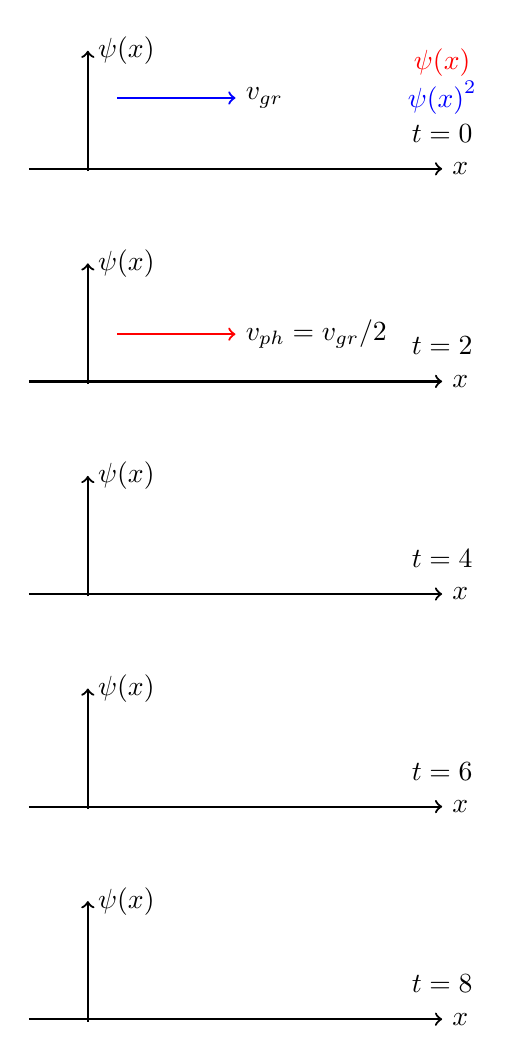
\begin{tikzpicture}[scale=0.15]
\draw[->,thick] (-5,0) -- (30,0) node[right]{$x$};
\draw[->,thick] (0,-.2) -- (0,10) node[right]{$\psi(x)$};
\sagestr{output1a}
\sagestr{output1b}
\draw[->,blue,thick] (2.5,6) -- (12.5,6) node[right,black]{$v_\rmt{gr}$};

\node at (30,3) {$t=0$};
\node[red] at (30,9) {$\psi(x)$};
\node[blue] at (30,6) {$\abs{\psi(x)}^2$};


\begin{scope}[shift={(0,-18)}]
\draw[->,thick] (-5,0) -- (30,0) node[right]{$x$};
\draw[->,thick] (0,-.2) -- (0,10) node[right]{$\psi(x)$};
\sagestr{output2a}
\sagestr{output2b}
\draw[->,red,thick] (2.5,4) -- (12.5,4) node[right,black]{$v_\rmt{ph} = v_\rmt{gr}/2$};
\node at (30,3) {$t=2$};
\end{scope}

\begin{scope}[shift={(0,-36)}]
\draw[->,thick] (-5,0) -- (30,0) node[right]{$x$};
\draw[->,thick] (0,-.2) -- (0,10) node[right]{$\psi(x)$};
\sagestr{output4a}
\sagestr{output4b}
\node at (30,3) {$t=4$};
\end{scope}

\begin{scope}[shift={(0,-54)}]
\draw[->,thick] (-5,0) -- (30,0) node[right]{$x$};
\draw[->,thick] (0,-.2) -- (0,10) node[right]{$\psi(x)$};
\sagestr{output6a}
\sagestr{output6b}
\node at (30,3) {$t=6$};
\end{scope}

\begin{scope}[shift={(0,-72)}]
\draw[->,thick] (-5,0) -- (30,0) node[right]{$x$};
\draw[->,thick] (0,-.2) -- (0,10) node[right]{$\psi(x)$};
\sagestr{output8a}
\sagestr{output8b}
\node at (30,3) {$t=8$};
\end{scope}

\end{tikzpicture}
\caption{The wavefunction and the magnitude of the wavefunction for time steps.}
\label{fig:gauspsi}
\end{marginfigure}

The Gaussian wave packet particle model predicts that the peak of the wave packet will move forward with average velocity $p_0/m$. However, there is another velocity in the phase of the wavefunction. Returning to Eq.~(\ref{Psi  G x t}), we plot the wavefunction and its magnitude in Figure~\ref{fig:gauspsi}. We see that there is also underlying velocity associated with the phase fronts that isn't visible in the probability density. Our Matter Wave Model actually predicts this. We go back to Eq.~(\ref{eq:tdsefreesolint})
\beq
\psi(x,t) = \sqrt{\frac{\hbar}{2\pi}}  \intii\phi(\hbar k,0) \E{\I(kx-\omega(k) t)}dk
\eeq
where $\omega(k) = \hbar k^2/2m$. We compare this to the Complex Electromagnetic Wave Amplitude Model we used in Section \ref{sec:CEWAM}. There are a couple of differences. Note that the angular frequencies of the two models are different:
\beq
\underbrace{\omega = c k\phantom{\frac{1}{\frac{1}{2}}}}_{\displaystyle \rmt{ElMaW}} \quad \longleftrightarrow \quad \underbrace{\omega = \frac{\hbar k^2}{2m\phantom{\frac{1}{2}}}}_{\displaystyle \rmt{MWM}},
\eeq
where $c$ is the speed of light in vacuum. 
We now define the phase velocity $v_{\rm ph}$ as the speed at which a definite wavelength plane wave travels:
%
\beq
v_{\rm ph} \equiv \frac{\omega(k)}{k}.
\eeq
%
For the light and matter waves, we find 
%
\begin{equation}
\underbrace{v_{\rm ph} = c}_{\displaystyle \rmt{ElMaW}} \phantom{space} \longleftrightarrow  \phantom{space} \underbrace{v_{\rm ph}  = \frac{\hbar k}{2m}}_{\displaystyle \rmt{MWM}}.
\end{equation}
%
As expected, we find that ElMaW plane wave travels the speed of light, but how do we interpret the matter wave phase velocity?  Using the relation between momentum $p_x$ and $k$, $p_x = \hbar k$, the matter wave phase speed is
%
\beq
v_{\rm ph} = \frac{p_x}{2m} = \frac{v_{\rm peak}}{2},
\eeq
%
where $v_{\rm peak} = p_x/m$ is the speed at which a the peak of the wave packet moves.  In our MWM, the definite momentum plane wave travels at a speed that is half what a particle with that momentum would travel.

There is another type of speed associated with a wave packet---the group velocity.  Because the Gaussian wave packet is composed of many plane waves with wave numbers centered around a particular value $k_{0}$, the wave travels at the group velocity $v_{\rm gr}$ defined by
%
\beq
v_{\rm gr} \equiv \left.\frac{d\omega}{dk}\right|_{k = k_{0}}.
\label{group velocity}
\eeq
%
The group velocity for the light and plane waves is then
%
\beq
\underbrace{v_{\rm gr} = c}_{\displaystyle \rmt{ElMaW}} \phantom{space} \longleftrightarrow  \phantom{space} \underbrace{v_{\rm gr}  = \frac{\hbar k_{0}}{m}}_{\displaystyle \rmt{MWM}},
\label{light matter group v}
\eeq
%
%
which is the wave packet peak velocity we found earlier. We see that our Gaussian wave packet matter wave model behaves in many respects like a classical particle.  A wave packet with a well-defined momentum $p_{0} = \hbar k_{0}$ will move undistorted at the group velocity $v_{\rm gr} = v_{\rm particle} = p_{0}/m$. Furthermore, if the momentum is very well-defined ($\sigma_{p}$ is small), the spread time $t_{\rm spread}$ is large, so it takes a long time for the wave to spread, hence the packet propagates with no significant distortion at the group velocity $p_{0}/m$.

\begin{exercise}
The energy $E$ of a spin-$0$ relativistic particle of mass $m$ and momentum $p$ is modeled by $E = \sqrt{m^{2}c^{4} + p^{2}c^{2}}$, where $c$ is the speed of light.  Using the relations $E = \hbar\omega$ and $p = \hbar k$, find the phase and group velocities associated with the quantum wave motion of such a system.  Express your answers in terms of the speed $v_{\rm particle}$ that a classical particle would travel with if it had the same mass and momentum.  Comment.
\end{exercise}

\section{Coherence Time and Length}

We saw that there is a characteristic time scale for our Gaussian wave packets: $t_\rmt{spread}$, Eq.~(\ref{t spread}). Since the wave packet is moving in space this also means that there is a characteristic length scale called the {\em coherence length}:\footnote{A more detailed discussion of some of these issues may be found in C. Cohen-Tannoudji and D. Gu\'{e}y-Odelin, {\em Advances in Atomic Physics} (World Scientific, Singapore, 2011), Chapter 17.} Although we treated the interfering matter waves in Chapter \ref{ch:mwmint} as large plane waves, a more accurate model is to describe them as Gaussian wave packets with large widths. There is another length scale that plays an important role in the MWM interference, especially in an interferometer. The {\em longitudinal coherence length} describes the length scale over which the wave packet maintains a relatively constant phase:
\beq
\ell_{c} \simeq  \frac{\hbar}{\sigma_{p}}.
\eeq
We wrote this with ``$\simeq$'' rather than ``$\equiv$'' because this is an approximate treatment. In order  to have diffraction and interference with slits of width $a$ and separation $d$, we need to have $\ell_{c} \gg a, d$. The same condition applies to any situation where we have interfering wave packets.


\section{Modified M-Z Interferometer}

We model the effect of a finite coherence length on the interference of matter waves in a modified Mach-Zehnder interferometer, shown in Figure \ref{modified M-Z setup}. We extended one path of the interferometer by inserting two mirrors and an extra path length $\Delta L$. The effect of adding the two mirrors on the overall phase is zero, since each mirror introduces a phase shift of $(-1)$. 

\begin{figure}
\centering
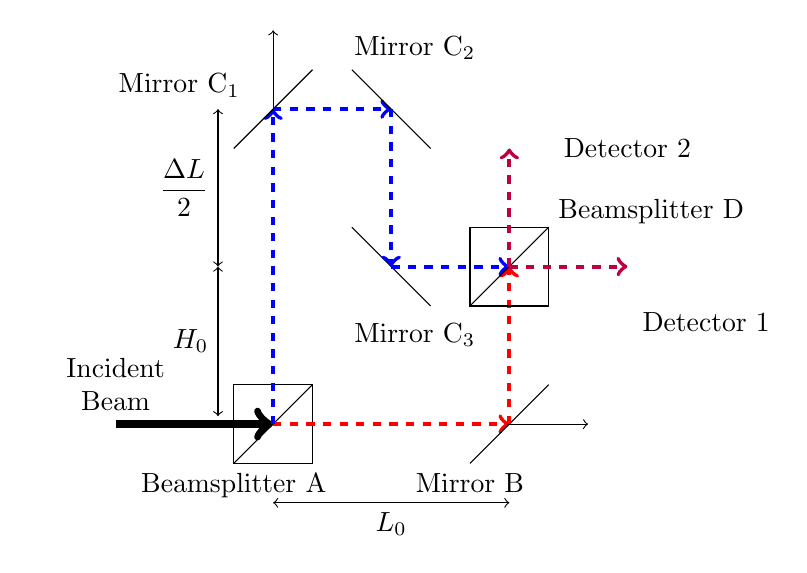
\begin{tikzpicture}
%beamsplitter 1
\draw (-0.5,-.5)node[below]{Beamsplitter A} rectangle +(1,1) ;
\draw (-.5,-.5) -- (.5,.5);


\draw[black,->,line width=3pt](-2,0)--(0,0) node[midway, above,shift=({-1cm,0}),text width=2cm,align=center]{Incident Beam};

%red beam
\draw[red,->,dashed,line width=1.5pt](0,0)--(3,0);
\draw (2.5,-.5)node[below]{Mirror B} -- (3.5,.5);
\draw[red,->,dashed,line width=1.5pt](3,0)--(3,2);
\draw[black,->](3,0) -- (4,0);

%blue beam
\draw[blue,->,dashed,line width=1.5pt](0,0)--(0,4);
\draw (-.5,3.5) node[left,shift={(0.2,.8)}]{Mirror C$_1$}-- (.5,4.5) ;
\draw[blue,->,dashed,line width=1.5pt](0,4)--(1.5,4);

\draw (2,3.5) node[above,shift={(-.2,1)}]{Mirror C$_2$} -- (1,4.5)  ;


\draw (2,1.5) node[below,shift={(-.2,-.1)}]{Mirror C$_3$}  -- (1,2.5);
\draw[blue,->,dashed,line width=1.5pt](1.5,4)--(1.5,2);

\draw[blue,->,dashed,line width=1.5pt](1.5,2)--(3,2);

\draw[->](0,4) -- (0,5);



\draw (2.5,1.5) rectangle +(1,1)node[above,right,shift={(0,.2)}]{Beamsplitter D} ;
\draw (2.5,1.5) -- (3.5,2.5);

%output beams
\draw[purple,->,dashed,line width=1.5pt](3,2) -- (3,3.5);
\draw[purple,->,dashed,line width=1.5pt](3,2) -- (4.5,2);

\detector{1}{4.5}{2}{0}
\node at (5.5,1.3) {Detector 1};

\detector{1}{3}{3.5}{90}
\node at (4.5,3.5) {Detector 2};

\draw[<->] (0,-1) -- (3,-1) node[midway,below]{$L_0$};

\draw[<->] (-.7,.1) -- (-.7,2) node[midway,left]{$H_0$};
\draw[<->] (-.7,2) -- (-.7,4) node[midway,left]{$\displaystyle \frac{\Delta L}{2}$};

\end{tikzpicture}
\caption[][1cm]{The modified Mach-Zehnder interferometer with a variable path length difference.}
\label{modified M-Z setup}
\end{figure}

The amplitude for a wave packet to arrive at Detector \#1 via path ABD is unchanged from Eq.~(\ref{psi ABD}):
\beq
\psi_{ABD} =  -\I\frac{1}{2}\E{\I k_{0}s_{0}}\E{\I k_{0}(L_{0} + H_{0})}.
\eeq
However, there is now an additional path length of $\Delta L$ in path ACD leading to an amplitude of
\beq
\psi_{ACD} = -\I\frac{1}{2}\E{\I k_{0}s_{0}}\E{\I k_{0}(L_{0} + H_{0})}\E{\I k_0 \Delta L}.
\eeq
So the overall probability density of the matter wave reaching Detector \#1 is \arnote[1cm]{Work out the missing steps.}
\beq
\Pd_1(\Delta L) = \abs{\psi_{ABD} + \psi_{ACD}}^2 = \frac{1}{2}\left[1+\cos(k_0\Delta L)\right],
\eeq
which we've graphed in Figure \ref{fig:pd1}.
\begin{marginfigure}
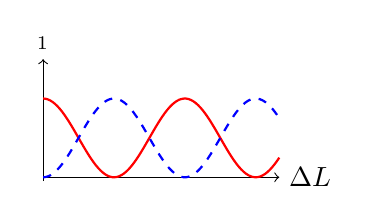
\begin{tikzpicture}[scale=0.5]
\draw[->](0,0) -- (6,0)node[right]{$\Delta L$};
\draw[->](0,-0.1) -- (0,3)node[above]{$\Pd_1$};
\draw[domain=0:6,samples=100,thick,red] plot({\x},{2/2*(1+cos(100*\x))});
\draw[domain=0:6,samples=100,thick,blue,dashed] plot({\x},{2/2*(1-cos(100*\x))});
\end{tikzpicture}
\caption{The probability density for measuring the wave at Detector 1 (solid) and Detector 2 (dashed).}
\label{fig:pd1}
\end{marginfigure}

\begin{exercise}
Show that the measurement probability density for Detector \#2 is
\beq
\Pd_2(\Delta L) =\frac{1}{2}\left[1-\cos(k_0\Delta L)\right].
\eeq
\end{exercise}


So if we have a single Gaussian wave packet incident on the interferometer, the wave packet splits into two packets traveling though the separate arms at velocity $v_\rmt{gr}$. Because path ABD is shorter, the wave packet traveling that arm will arrive at beamsplitter D first. If the path length difference between the two arms is large compared to the coherence length, $\Delta L \gg \ell_c$, then the wave packets will not overlap at the beamsplitter and will not interfere.

We model this using a fixed Gaussian momentum probability density (Eq.~(\ref{P G p})) along the direction of motion ($s$) of the beams:
\beq
\Pd_{G,p}(p_{s})  =  \frac{1}{\sigma_{p}\sqrt{2\pi}}\E{-(p_{s} - p_{0})^{2}/(2\sigma_{p}^{2})}.
\eeq
Because we know the probability density of measuring the beam at Detector \#1, we can integrate over all possible momenta to find the total probability (where $k_0 = p_s/\hbar$ is the wave packet central momentum):
\bas
P_1(\Delta L) = & \intii \Pd_{G,p}(p_s) \Pd_1(p_s,\Delta L) dp_s  \\
 = & \intii \frac{1}{\sigma_{p}\sqrt{2\pi}}\E{-(p_{s} - p_{0})^{2}/(2\sigma_{p}^{2})} \frac{1}{2}\left[1+\cos(\frac{p_s\Delta L}{\hbar})\right]dp_s \\
 =&\frac{1}{2} + \frac{1}{2}\cos\left(\frac{p_0 \Delta L}{\hbar}\right)\exp\left[-\frac{1}{2}\left(\frac{\Delta L}{\ell_c}\right)^2\right] \label{eq:probdet1gaus}
\eas\arnote[-1.5cm]{Fill in the missing steps. Use your \CAS if you want. I did.}%
where we've substituted the coherence length $\ell_c = \hbar/\sigma_p$ in for the wave packet width.

This is the same probability density we found earlier for long coherence lengths (or short path-length differences). However, as the relative path length difference increases, we see that the fringe contrast decreases eventually to the point where the interference pattern disappears as we see in Figure \ref{fig:pdloss}.

\begin{marginfigure}[-2cm]
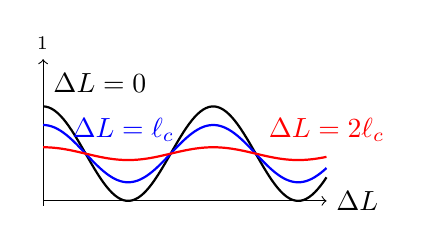
\begin{tikzpicture}[scale=0.6]
\draw[->](0,0) -- (6,0)node[right]{$\Delta L$};
\draw[->](0,-0.1) -- (0,3)node[above]{$\Pd_1$};
\draw[domain=0:6,samples=100,thick,black] plot({\x},{2/2*(1+cos(100*\x))});
\draw[domain=0:6,samples=100,thick,blue] plot({\x},{2/2+cos(100*\x)*exp(-1/2)});
\draw[domain=0:6,samples=100,thick,red] plot({\x},{2/2+cos(100*\x)*exp(-1/2*4)});
\node[black] at (1.2,2.5) {$\Delta L = 0$};
\node[blue] at (1.7,1.5) {$\Delta L = \ell_c$};
\node[red] at (6,1.5) {$\Delta L = 2\ell_c$};
\end{tikzpicture}
\caption{The probability density for measuring the wave at Detector 1 for increasing $\Delta L$.}
\label{fig:pdloss}
\end{marginfigure}

\begin{exercise}
 Suppose you wish to do an interference experiment using the modified Mach-Zehnder interferometer using sodium atoms.  If $\Delta L \simeq 1$~mm, estimate the minimum spread in velocities about the average $v_{0}$  within the atomic beam  allowed in order to see strong interference.
\end{exercise}

\begin{exercise}
The {\em visibility} ${\cal V}$, which measures the contrast between the interference maxima and minima, is used to characterize the amount of interference of a system:
%
\begin{equation}
{\cal V} = \frac{I_{\rm max} - I_{\rm min}}{I_{\rm max} + I_{\rm min}}.
\label{V}
\end{equation}
%
Here $I_{\rm max}$ and $I_{\rm min}$ are maximum and minimum intensities, respectively, that are observed by a detector as some parameter is varied.  Since the measured intensity is proportional to the probability of detection ($I \propto \Pd$), we can recast Eq.~(\ref{V}) as 
%
\begin{equation}
{\cal V} = \frac{\Pd_{\rm max} - \Pd_{\rm min}}{\Pd_{\rm max} + \Pd_{\rm min}},
\label{V2}
\end{equation}
%
where $\Pd_{\rm max}$ and $\Pd_{\rm min}$ are   maximum and minimum probability densitites, respectively, that are observed by a detector as some parameter is varied. 

\begin{enumerate}
\item[(a)] Show that $0 \leq {\cal V} \leq 1$.  What happens  to the interference when  ${\cal V} = 0$?  When  ${\cal V} = 1$? 
\item[(b)]  Use Eq.~(\ref{eq:probdet1gaus}) to find ${\cal V}$ for interference observed by detector \#1 as $\Delta L$ is varied for the modified Mach-Zehnder interferometer.  For what values of $\Delta L$ is  ${\cal V} = 0$?  For what values of $\Delta L$ is   ${\cal V} = 1$? 

\end{enumerate}


\end{exercise}




%---------------------------------------
\chapter{Motion in a Constant Potential}

We are now going to move from the free space Hamiltonian model to develop models where our quantum systems experience external potentials. Again we begin with the Schr\"{o}dinger equation
\beq
\I\hbar\frac{\partial}{\partial t}\ket{\Psi} = \hat{H}\ket{\Psi}.
\eeq\marginnote[-.8cm]{\ref{tool:sch}}%
But now the total mechanical energy consists of both the kinetic energy and a potential energy. We will limit our model to situations where the potential energy is not time-dependent. We will also now develop a model for describing three-dimensional systems.

\section{Three-Dimensional Wavefunctions and Operators}

\subsection{Position Operator and Wave Function}
So far we've confined our discussion to just one dimension, but everything we have done can be extended to three dimensions.  First, let's look at position, where we can introduce observables $\hat{X}$, $\hat{Y}$, and $\hat{Z}$  for each of the three Cartesian coordinates $x$, $y$, and $z$.  The eigenvalue equations for each are then
%
\bas
\hat{X}\ket{x} & =  x\ket{x}, \label{x equation} \\
\hat{Y}\ket{y} & =  y\ket{y}, \label{y equation} \\
\hat{Z}\ket{z} & =  z\ket{z}, \label{z equation}
\eas\marginnote[-1.5cm]{\ref{tool:eigen}}%
where $\ket{x}$, $\ket{y}$, and $\ket{z}$ are the eigenvectors associated with the eigenvalues $x$, $y$, and $z$, respectively.  We write the  position $j$-component as $x_{j}$, where $j = 1, 2, 3$ with $1 = x$, $2 = y$, and $3 = z$ as a more compact notation.  Then we can write Eqs.~(\ref{x equation})--(\ref{z equation}) as
%
\beq
\hat{X}_{j}\ket{x_{j}} = x_{j}\ket{x_{j}}.
\eeq
% 

Whenever we have more than one observable, we should ask the question:  do the observables commute with each other?  We will limit our model to the situation where 
%
\beq
\com{\hat{X}_{j}, \hat{X}_{k}} = 0
\label{XX commute}
\eeq\marginnote[-0.8cm]{\ref{tool:commutator}}%
for all $j,k = x, y, z$.  \marginnote{ It is hard to imagine this not being zero, but mathematicians have developed a whole field called noncommutative geometry which utilizes non-commuting position components.  In addition, there are good reasons to believe that our macroscopic view of space and time might breakdown at a sufficiently small scale.} Physically, this means we can locate a our quantum system in space in all three dimensions to arbitrarily small precision.  Mathematically, it means that we can find a common set of eigenvectors for all three observables.  We denote these eigenvectors by $\ket{xyz}$ where 
%
\bas
\hat{X}\ket{xyz} & =  x\ket{xyz},  \\
\hat{Y}\ket{xyz} & =  y\ket{xyz},  \\
\hat{Z}\ket{xyz} & =  z\ket{xyz}. 
\eas
%

We simplify the notation a bit more by defining the 3-dimensional position eigenvector in a hybrid 3-vector/state vector notation as
%
\beq
\ket{\vec{r}} \equiv \ket{xyz}
\eeq
%
with normalization
%
\beq
\avg{\vec{r}|\vec{r}\,'} = \delta(\vec{r} - \vec{r}\,').
\eeq
%
Here the 3-dimensional Dirac delta function $\delta(\vec{r} - \vec{r}\,')$ is defined by \marginnote{The integral $ \int d^{3}r$ means we are integrating over all space.}
%
\bas
f(\vec{r}\,') & = \int  f(\vec{r}) \delta(\vec{r} - \vec{r}\,') d^{3}r,
\nonumber \\
 & =   \int^{\infty}_{-\infty} \int^{\infty}_{-\infty} \int^{\infty}_{-\infty}\,f(x,y,z)\delta(x - x')\delta(y - y')\delta(z - z') dx\,dy\,dz,
\eas
%
where $f(\vec{r})$ is an arbitrary function in 3-dimensional space.


We can define a 3-vector observable  $\hat{\vec{R}}$ which is the operator analog of the position vector $\vec{r} = x\hat{x} + y\hat{y} + z\hat{z}$:\marginnote{Warning:  We are using ``\,\,$\hat{\mbox{}}$\,\,'' to denote both an operator and a unit vector! Recall that upper-case means operator in our notation.}
%
\beq
\hat{\vec{R}} \equiv  \hat{X}\hat{x} +\hat{Y}\hat{y} + \hat{Z}\hat{z}.
\eeq
%
This will be useful for writing the potential energy of systems in three dimensions.  Then 
%
\beq
\hat{\vec{R}}\ket{xyz} = \left(x\hat{x} + y\hat{y} + z\hat{z}\right)\ket{xyz},
\eeq
%
or compactly,
%
\beq
\hat{\vec{R}}\ket{\vec{r}} = \vec{r}\ket{\vec{r}}.
\eeq\marginnote[-1.5cm]{\ref{tool:eigen}}%
%
The matrix elements of $\hat{\vec{R}}$ in the position basis are
%
\beq
\bra{\vec{r}}\hat{\vec{R}}\ket{\vec{r}\,'} = \vec{r}\,'\delta(\vec{r} - \vec{r}\,').
\eeq
%

The completeness relation for three dimensions is
%
\beq
 \onehat =  \int\,\ket{\vec{r}}\bra{\vec{r}}
d^{3}r =  \iiint\displaylimits^{\infty}_{-\infty}\,\ket{xyz}\bra{xyz}\,dx\,dy\,dz.
\label{3-D position completeness relation}
\eeq
%
If we apply this to an arbitrary state vector $\ket{\Psi}$ describing a particle in three dimensions, we have
%
\bas
\ket{\Psi} & =  \onehat\ket{\Psi}, \\
& =  \int \ket{\vec{r}}\avg{\vec{r}|\Psi} d^{3}r, \\
& =   \int  \,\psi(\vec{r})\ket{\vec{r}} d^{3}r,
\eas
%
where the 3-dimensional position wave function is
%
\beq
\psi(\vec{r}) \equiv \avg{\vec{r}|\Psi}.
\eeq\marginnote[-0.8cm]{This joins the \ref{tool:wavefunction}.}
%
The 3-dimensional position probability density $\Pd(\vec{r})$ is related to $\psi(\vec{r})$ by
%
\beq
\Pd(\vec{r}) = \abs{\psi(\vec{r})}^{2},
\eeq
%
where $\Pd(\vec{r})d^{3}r = \Pd(x,y,z)dxdydz$ is the probability the system will be measured in the volume $x$ to $x + dx$, $y$ to $y + dy$, and $z$ to $z + dz$.  Since the probability of finding the state somewhere is unity, $\Pd(\vec{r})$ must satisfy the normalization condition:
%
\beq
\int\, \Pd(\vec{r}) d^{3}r = 1.
\eeq

The way we apply the rules of quantum mechanics generalize in a sensible manner from the 1-dimensional cases we have already investigated.  This is most easily demonstrated by an example:


\begin{exercise}
\label{ex:sphericalpotential1}
Suppose an atom is equally likely to found anywhere inside a sphere of radius $R$ centered at the origin, and will not be found outside the sphere.  Show that the wave function characterizing such an atom can be written as
%
\beq
\psi(\vec{r}) = \begin{cases}\displaystyle \frac{1}{\sqrt{V_{0}}} & r \leq R, \\ 0 & r > R, \end{cases}
\label{uniform psi}
\eeq
%
where $V_{0} = (4/3)\pi R^{3}$ is the volume of the sphere and $r = \abs{\vec{r}}$ is the distance from the origin.  
\end{exercise}



\subsection{Non-Cartesian Coordinate Systems}
\label{sec:noncartesisanone}
At this stage you might wonder about defining position component operators for non-Cartesian coordinates.  For example, if one wants to use spherical coordinates, does it make sense to define operators corresponding to the components ($r, \theta, \varphi$):
%
\begin{equation}
 (\hat{X}, \hat{Y}, \hat{Z}) \rightarrow (\hat{R}, \hat{\Theta}, \hat{\varphi})?
\end{equation}
%
It turns out that there are plenty of technical issues with this so, for now, we adopt Shankar's approach\footnote{R. Shankar, {\em Principles of Quantum Mechanics}, 2nd ed., (Plenum, NY, 1994), pp.~141--143, and 214--216.} and will stick to using Cartesian coordinates.  If we need to switch to other coordinate systems, we will obtain the needed wave equation in Cartesian coordinates using the Cartesian position (and momentum) operators, and then use a conventional change of coordinates to obtain the form in the desired coordinate system.  This will get us to the same result as obtained by a more complicated approach.


\begin{example}
An atom is equally likely to found anywhere inside a sphere of radius $R$ centered at the origin, and will not be found outside the sphere.  What is the probability that it will be found in the region $R/2 \leq r \leq R$ and $0 \leq \theta \leq \pi/2$? 

\model We will model the atom as a quantum system and we'll use spherical coordinates where $r$ is the radial coordinate, $\theta$ is the angle measured from the $+z$-axis, and $\varphi$ is the azimuthal angle.

\vis We're looking for the the probability of measuring the atom in this region (where this is actually a sphere and we're looking at almost all of the top hemisphere.) This is show in Fig.~\ref{fig:261}.
\begin{figure}
\centering
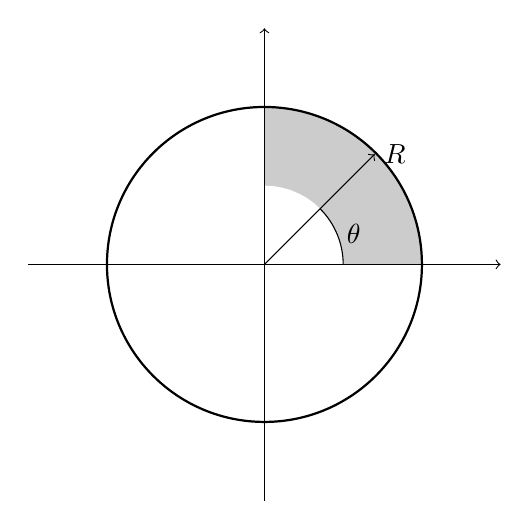
\begin{tikzpicture}
\begin{scope}
\clip (0,0) rectangle(2,2);
\fill[black!20] (0,0)circle(2);
\end{scope}
\draw[thick] (0,0) circle(2);
\fill[white] (0,0) circle(1);
\draw[->](-3,0) -- (3,0);
\draw[->](0,-3) -- (0,3);
\draw[->] (0,0) -- (1.4,1.4) node[above,right] {$R$};
\draw (1,0) arc (0:45:1) node[midway,right]{$\theta$};


\end{tikzpicture}
\caption[][2cm]{ }
\label{fig:261}
\end{figure}

\sol 
We integrate the position probability density $\Pd(\vec{r}) = \abs{\psi(\vec{r})}^{2}$ over the allowed region of space, remembering that for spherical coordinates, $d^{3}r = r^{2}\sin\theta\,dr\,d\theta\,d\varphi$:\arnote{Do the integrals out in your notes.}
%
\bas
P\left(\frac{R}{2} \leq r \leq R,0 \leq \theta \leq \frac{\pi}{2}\right)  = & \int_{\rm allowed} \,\abs{\psi(\vec{r})}^{2} d^{3}r  \\
 = & \int^{R}_{R/2}\,\frac{1}{V_{0}}r^{2}dr\int^{\pi/2}_{0}\sin\theta d\theta\,\int^{2\pi}_{0}d\varphi\, \nonumber \\
 = & \frac{7}{16}.
\eas

Now suppose we measure the atom in this region.  What is the state of the atom after the measurement?  We need to take the state prior to the measurement, $\psi(\vec{r})$, remove all parts not consistent with the measurement, and then renormalize the result.  Since the probability of finding it in the desired region is $7/16$, the normalization factor is $\sqrt{16/7}$ so the state immediately the measurement is
%
\beq
\psi_{\rm after}(\vec{r}) = \begin{cases}\displaystyle \sqrt{\frac{12}{7\pi R^{3}}}, \,\,\,\,\, & \displaystyle \frac{R}{2} \leq r \leq R, 0 \leq \theta \leq \frac{\pi}{2}, \\  
& \\ 0, & \mbox{elsewhere}. \end{cases}
\eeq

\assess The measurement probability is reasonable given that we're looking at almost all of the top hemisphere area.

\end{example}

\subsection{Momentum in 3-Dimensional Space}

Most of the results from position in three dimensions obtained in the previous section can be carried over directly to momentum simply by replacing $x_{j} \rightarrow p_{j}$ and $\hat{X}_{j} \rightarrow \hat{P}_{j}$, where $j = x,y,z$. 

The momentum eigenvalue equation for the $i$th direction is%
\beq
\hat{P}_{j}\ket{p_j} = p_{j}\ket{p_j},
\eeq\marginnote[-0.8cm]{\ref{tool:eigen}}%
% 
where the momentum operators are assumed to commute among themselves:
%
\beq
\com{\hat{P}_{j}, \hat{P}_{k}} = 0.
\label{PP commute}
\eeq\marginnote[-0.7cm]{\ref{tool:commutator}}%
In addition, we see that the position-momentum commutation relationships are 
%
\beq
\com{\hat{X}_{j}, \hat{P}_{k}} = \I\hbar\delta_{jk},
\label{XP commute}
\eeq\marginnote[-0.7cm]{\ref{tool:commutator}}%
so that the Heisenberg uncertainty principle in three dimensions is
%
\beq
\Delta X_{j}\Delta P_{k} \geq \frac{\hbar}{2}\delta_{jk}.
\eeq\marginnote[-0.7cm]{\ref{tool:genuncert}}%
Therefore, it is possible to know the $x$-component of a particle's position and $y$-component of its momentum with arbitrary precision simultaneously, but not the $x$-components of both quantities.

Just as we did with position, we define a momentum vector operator
\beq
\hat{\vec{P}}\ket{\vec{p}} =\vec{p}\ket{\vec{p}},
\eeq\marginnote[-0.7cm]{\ref{tool:eigen}}%
where
\beq
\ket{\vec{p}} = \ket{p_{x}p_{y}p_{z}}
\eeq%
represents the state of a particle with definite momentum $\vec{p}$.  The matrix elements of the momentum operator relative to the position basis are the 3-dimensional analog of the 1-dimensional case:\marginnote{Note that $\vec{\nabla}$ is the three-dimensional derivative vector.}
%
\beq
\bra{\vec{r}}\hat{\vec{P}}\ket{\vec{r}\,'} = -\I\hbar\delta(\vec{r}-\vec{r}\,')\vec{\nabla}'.
\eeq

If we apply the  3-dimensional  completeness relation for momentum states, \marginnote{Again, the integral $ \int d^{3}p$ means we are integrating overall all possible momenta. }
%
\beq
 \onehat =  \int \,\ket{\vec{p}}\bra{\vec{p}}d^{3}p 
=  \intii dp_{x} \intii dp_{y} \intii dp_{z}\,\ket{p_{x}p_{y}p_{z}}\bra{p_{x}p_{y}p_{z}},
\eeq
%
to an arbitrary state vector $\ket{\Psi}$, we obtain
%
\bas
\ket{\Psi} & =    \onehat \ket{\Psi} =  \int \,\ket{\vec{p}}\avg{\vec{p}|\Psi}d^{3}p  \\
& =   \int  \,\phi(\vec{p})\ket{\vec{p}}  d^{3}p,
\eas
%
where the 3-dimensional momentum wave function is
%
\beq
\phi(\vec{p}) \equiv \avg{\vec{p}|\Psi}.
\eeq\marginnote[-0.8cm]{This also joins the \ref{tool:wavefunction}.}
%
The 3-dimensional momentum probability density $\Pd_{p}(\vec{p})$ is related to $\phi(\vec{p})$ by
%
\beq
\Pd_{p}(\vec{p}) = \abs{\phi(\vec{p})}^{2},
\eeq
%
where $\Pd_{p}(\vec{p})d^{3}p = \Pd_{p}(p_{x},p_{y},p_{z})dp_{x}dp_{y}dp_{z}$ is the probability the state will be measured with momentum in the range $p_{x}$ to $p_{x} + dp_{x}$, $p_{y}$ to $p_{y} + dp_{y}$, and $p_{z}$ to $p_{z} + dp_{z}$.

\subsection{Relations between Position and Momentum Wave Functions}

We saw earlier that, in 1-dimension, the position and momentum wave functions were related to each  other via the generalized Fourier transform.    This can be generalized to 3-dimensions by applying that result to each coordinate.  For example, the 3-dimensional momentum wave function $\phi(\vec{p})$ is related to the 3-dimensional wave function $\psi(\vec{r})$ by using a 3-dimensional version of Eq.~(\ref{eq:ftxtop}):
\beq
\phi(\vec{p}) = \left(\frac{1}{\sqrt{2\pi\hbar}}\right)^{3}\intii dx \intii dy\intii dz\,\psi(x,y,z)\E{-\I p_{x}x/\hbar}e^{-\I p_{y}y/\hbar}e^{-\I p_{z}z/\hbar},
\eeq
%
which can be simplified to
%
\beq
\displaystyle \phi(\vec{p}) = \frac{1}{(2\pi\hbar)^{3/2}}\int \psi(\vec{r})\E{-\I\vec{p}\cdot \vec{r}/\hbar}d^{3}r.
\label{phi psi relation}
\eeq\marginnote[-1cm]{\ref{tool:FTtool}}
%
Similarly, the inverse relation is a generalized version of Eq.~(\ref{eq:ftptox})%
\beq
\displaystyle \psi(\vec{r}) = \frac{1}{(2\pi\hbar)^{3/2}}\int \phi(\vec{p})\E{\I\vec{p}\cdot \vec{r}/\hbar}d^{3}p.
\eeq\marginnote[-0.8cm]{\ref{tool:FTtool}}
%

\begin{example}
What is the momentum wave function for the position wave function given by Eq.~(\ref{uniform psi}):
%
\beq
\psi(\vec{r}) = \begin{cases}\displaystyle \frac{1}{\sqrt{V_{0}}} & r \leq R, \\ 0 & r > R, \end{cases}
\eeq

\model We model the wavefunction as normalized and over the sphere. We'll use the modified Fourier transform to get the momentum wavefunction. It makes sense to use spherical coordinates again. It also makes sense to pick the coordinate system so that the momentum points along the $z$-direction: $\vec{p} = p\hat{z}$.

\vis The picture hasn't changed.

\sol We have
%
\beq
\phi(\vec{p}) = \frac{1}{(2\pi\hbar)^{3/2}} \int^{R}_{0}\frac{1}{\sqrt{V_{0}}}r^{2} dr\,\int^{\pi}_{0}\sin\theta d\theta\,\int^{2\pi}_{0}d\varphi\,\E{-\I\vec{p}\cdot \vec{r}/\hbar}.
\label{example phi 1}
\eeq
%
Since the momentum points in the $z$-direction, 
\begin{equation}
\vec{p}\cdot\vec{r} = pr\cos\theta.
\end{equation}
%
so  Eq.~(\ref{example phi 1}) becomes
%
\beq
\phi(\vec{p})  =  \frac{1}{(2\pi\hbar)^{3/2}} \int^{R}_{0}dr\,r^{2}\int^{\pi}_{0}d\theta\,\sin\theta\,\int^{2\pi}_{0}d\varphi\,\frac{1}{\sqrt{V_{0}}}e^{-ipr\cos\theta/\hbar}
\eeq
where $V_{0} = (4/3)\pi R^{3}$. This gives\arnote{Be sure to fill in these skipped steps.}
\beq
\phi(\vec{p}) = \sqrt{\frac{3R^{3}}{2\pi^{2}\hbar^{3}}}
 \left[\left(\frac{\hbar}{pR}\right)^{3}\sin\left(\frac{pR}{\hbar}\right) -  \left(\frac{\hbar}{pR}\right)^{2} \cos\left(\frac{pR}{\hbar}\right)\right].
\label{example phi final}
\eeq
%
\begin{marginfigure}

\begin{sagesilent}
x=var('x')
t = var('t')
x_coords = [t for t in srange(0.01,6.0,.1)]
y_coords = [15*((1/t)^3 *sin(t) - (1/t)^2 * cos(t))^2 for t in srange(0.01,6.0,.1)]
output = ""
for i in range(0,len(x_coords)-1):
    output += r"\draw[red, thick] (%f cm ,%f cm)--(%f cm ,%f cm);"%(x_coords[i],y_coords[i],x_coords[i+1],y_coords[i+1])
\end{sagesilent}

\begin{tikzpicture}[scale=0.8]
\draw[->](0,0) -- (6,0) node[right]{$pR/\hbar$};
\draw[->](0,0) -- (0,3) node[above]{$\abs{\phi}$};
\sagestr{output}
\end{tikzpicture}
\caption{The momentum probability density obtained from Eq.~(\ref{example phi final}). }
\label{Example phi graph}
\end{marginfigure}

\assess The units work out - we have [1/momentum$^{(3/2)}$] which are the units for the 3D momentum wavefunction. The momentum probability density $\Pd_{p}(\vec{p})$ obtained from this momentum wave function is shown in Fig.~\ref{Example phi graph}.   Since $\psi(\vec{r})$ is spherically symmetric in this example, we see that $\phi(\vec{p})$ only depends on $p$ and not on the direction of the momentum; momenta of all directions are equally likely.  We note that the width of ${\cal P}_{p}(\vec{p})$ is $\sim \hbar/R$, as expected by the Heisenberg uncertainty principle since $\Delta r \sim R$, where $\Delta r$ is ``uncertainty'' of the radial coordinate.  [Note that since we have not defined a radial coordinate operator, we don't have an uncertainty relation of the form $\Delta r\Delta p \geq \hbar/2$.]

\end{example}

\begin{exercise}
Check that $\phi(\vec{p})$ given by Eq.~(\ref{example phi final}) is properly normalized:
%
\begin{equation}
\int d^{3}p\, \abs{\phi(\vec{p})}^{2} = 1.
\end{equation}

\end{exercise}

\section{3D Schr\"{o}dinger Equation}

We are now equipped to talk about a system with total energy $H = p^2/2m + V(\vec{r})$. \marginnote{In 3D, the kinetic energy is $(\vec{p}\cdot\vec{p})/(2m) = p^2/(2m)$ where the momentum squared is now explicitly $p^2 = p_x^2 + p_y^2 + p_z^2$. \ref{tool:sch}} We now model this total energy as an operator in the position basis:
\beq
\bra{\vec{r}}\I\hbar\frac{\partial}{\partial t}\ket{\Psi} =  \bra{\vec{r}}\hat{H}\ket{\Psi}.
\eeq
The Hamiltonian operator in the position basis now has two components: the kinetic energy operator and the potential energy operator. Our model will only have the potential energy depend on position, so we will replace every position variable in the potential energy with the corresponding position operator.  We will denote this as $V(\hat{\vec{R}})$. The Hamiltonian in the position basis is thus
\bas
\bra{\vec{r}}\hat{H}\ket{\vec{r}\,'} = & \frac{1}{2m}\bra{\vec{r}}\hat{\vec{P}}^2\ket{\vec{r}\,'} + \bra{\vec{r}}V(\hat{\vec{R}})\ket{\vec{r}\,'} \\
= &  -\frac{\hbar^2}{2m}\vec{\nabla}^2 + V(\vec{r}) 
\eas
because the position state-vectors are eigenvalues of the position operator. That gives us the Time-Dependent Schr\"{o}dinger Wave Equation (TDSWE) :
\beq
\I\hbar \frac{\partial \psi(\vec{r},t)}{\partial t} =-\frac{\hbar^2}{2m}\vec{\nabla}^2\psi(\vec{r},t) + V(\vec{r}) \psi(\vec{r},t).
\label{eq:TDSWE}
\eeq\toolnote[-2.5cm]{\toollabel{tool:TDSWE}{\includegraphics{tool13.tikz} {\bf TDSWE}}  This tool is used to find the time evolution of a quantum wavefunction in the position basis in a position-dependent potential.} 
Because the Hamiltonian is time-independent, we can, in principle, find energy eigenvectors $\ket{\psi_E}$ and eigenvalues $E$ such that
\beq
\hat{H}\ket{\psi_E} = E\ket{\psi_E} \rmt{ where } \psi(\vec{r}) = \avg{\vec{r}|\psi_E}.
\eeq
We project this onto the position basis and we get the Time-Independent Schr\"{o}dinger Wave Equation (TISWE):
\beq
-\frac{\hbar^2}{2m}\vec{\nabla}^2\psi_E(\vec{r}) + V(\vec{r}) \psi_E(\vec{r})= E \psi_E(\vec{r})
\label{eq:TISWE}
\eeq\toolnote[-2.5cm]{\toollabel{tool:TISWE}{\includegraphics{tool14.tikz} {\bf TISWE}}  This tool is used to find the energy eigenvalues for a the time-independent Schr\"{o}dinger equation in the position basis.}%
And we can build up general time-dependent solutions out of a linear combination of these eigenvectors
\beq
\ket{\Psi} = \sum_E a_E \E{-\I E t/\hbar}\ket{\psi_E} \rmt{ where } a_E = \avg{\psi_E|\Psi(\vec{r},t=0)},
\eeq
or, in terms of wavefunctions,
\beq
\psi(\vec{r},t) = \sum_E a_E \E{-\I E t/\hbar}\psi_E(\vec{r})
\eeq


\section{Constant Potential}
\label{sec:constpotential}
So what happens if $V(\vec{r}) = V_0$, a constant? This is a model of an experiment where there are no external forces acting on a system. Examples could be an atom moving in a horizontal plane or an electron confined to a flat 2D surface. Another example could be a system in a material with a constant background potential. In this case the TISWE (Eq.~(\ref{eq:TISWE})) becomes
\beq
-\frac{\hbar^2}{2m}\vec{\nabla}^2\psi_E(\vec{r}) + V_0 \psi_E(\vec{r})= E \psi_E(\vec{r}).
\eeq
We move the constant potential to the right-hand side and define a new {\em effective energy} $E_\rmt{eff} = E - V_0$. The TISWE is thus
\beq
-\frac{\hbar^2}{2m}\vec{\nabla}^2\psi_E(\vec{r})= E_\rmt{eff} \psi_E(\vec{r})
\eeq
which is exactly the same as the situation as we saw in Section \ref{sec:FSHam} for the free-space Hamiltonian. All of the work we did for describing those states now apply here. We get energy eigenfunctions 
\beq
\psi_E(\vec{r}) = A\E{\I \vec{k}\cdot\vec{r}} \rmt{ where } E_\rmt{eff} = \frac{\hbar^2 k^2}{2m}.
\eeq
This means that the energy eigenvalues of the TISWE are shifted from the free-space model by the constant potential:
\beq
E = \frac{\hbar^2 k^2}{2m} + V_0.
\eeq

\begin{exercise}
Write down the TDSWE that you would need to solve to find the motion of a quantum mechanical atom of mass $m$ in the following situations:
\begin{enumerate}
\item An atom in the Earth's gravitational field at height $z$ above the ground.  (Show a sketch of your setup and coordinate system.)
\item A neutron on a frictionless plane connected to a wall with a spring with force constant $k$. (Show a sketch of your setup and coordinate system.)
\end{enumerate}

\end{exercise}

\begin{exercise}
Consider an electron characterized by a wave packet with average energy $E_{0}$ in a material characterized by a constant potential $V_{0}$.  

\begin{enumerate}
\item Find the average wave number $k_{0}$ associated with this packet.
\item  Find the group velocity of this packet, expressing your answer in terms of $E_{0}$ instead of $k_{0}$.\marginnote{Recall that $E = \hbar \omega$.}
\item Does the packet travel faster or slower in the material when compared to a free electron ($V_{0} = 0$) having the same average energy?  Does this make sense? 
\end{enumerate}

\end{exercise}





%---------------------------------------
\chapter{Quantum Scattering}
\label{ch:scattering}

We now model what happens if, instead of a constant potential, there is an abrupt change in potential. This is a simple model for the situation like a finite wire. We use the MWM to describe the electron motion in the wire. However, when the electron reaches the end of the wire, the potential shifts. We will first model a single change in the potential, then we will look at what happens if the potential shifts a second time.

\section{Potential Barrier}
We begin with a potential barrier model for the change in potential due to the end of a finite wire. We use the MWM to describe an electron in the wire that reaches the potential barrier at the end. We model the matter wave as approaching the barrier from the left with an energy $E$ larger than the barrier potential height $V_0$.%
\begin{marginfigure}
\centering
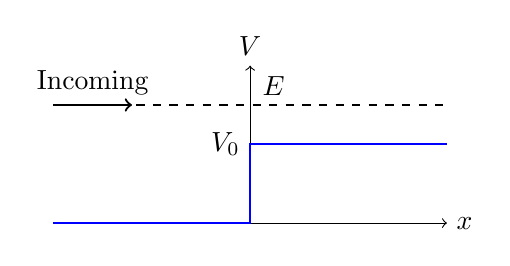
\begin{tikzpicture}
\draw[->](-2.5,0) -- (2.5,0) node[right]{$x$};
\draw[->](0,0) -- (0,2)node[above]{$V$};
\draw[blue,thick] (-2.5,0) -- (0,0) -- (0,1)node[left,black]{$V_0$} -- (2.5,1);
\draw[dashed](-2.5,1.5) -- (0,1.5) node[above,shift={(.3,0)}]{$E$} --(2.5,1.5);
\draw[->,thick](-2.5,1.5) -- (-1.5,1.5)node[midway,above]{Incoming};
\end{tikzpicture}
\end{marginfigure}%
In the region $x<0$, the MWM eigenstates are the momentum eigenstates we found in Section \ref{sec:FSHam}. The quantum state wavefunction in the position basis, as a function of time, is the result we found in Eq.~(\ref{eq:tdsefreesol})
\beq
\Psi(x,t) \propto \E{\I (k x -\omega t)}, \rmt{ where } k^2=\frac{2mE}{\hbar^2} \rmt{ and } \omega = \frac{\hbar k^2}{2m}.
\eeq
Similarly, in the region $x>0$, the MWM eigenstates are the energy-shifted eigenstates we found in Section \ref{sec:constpotential}. The wave number shifts, as does the total energy. The eigenstates are 
\beq
\Psi(x,t) \propto \E{\I (k' x -\omega' t)}, \rmt{ where } k'^2=\frac{2m(E - V_0)}{\hbar^2} \rmt{ and } \omega' = \frac{\hbar k'^2}{2m}.
\eeq\arnote[-1cm]{Fill in these missing steps.}
As we've noted before, these wavefunctions are not normalizable: the integral over all space is infinite. However, we can construct Gaussian wave packets to make normalizable states. We are interested, though, in the probability of measuring the state in either of the two regions of interest. We use a {\em probability current} model to describe these probabilities and how they relate to each other, even though we do not normalize the overall probability.


\section{Probability Current}
We are interested in the time-rate of change of the measurement probability:
\beq
\frac{d}{dt}\avg{\Psi|\Psi}?
\eeq
If we model our state as being normalized (for example, using Gaussian wave packets), this is zero - the total probability doesn't change in time. However, we can ask how the probability of measuring the state in a specific region (from $x=a$ to $x=b$) changes in time:%
\begin{marginfigure}
\centering
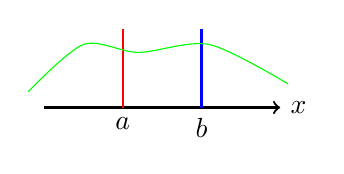
\begin{tikzpicture}
\draw[->,thick] (0,0) -- (3,0) node[right]{$x$};
\draw[red,thick] (1,0)node[below,black]{$a$} -- (1,1);
\draw[blue,thick] (2,0)node[below,black]{$b$} -- (2,1);
\draw [green] plot [smooth] coordinates {(-.2,.2) (.5,.8) (1.2,.7) (2.1,.8) (3.1,.3)};
\end{tikzpicture}
\end{marginfigure}%
\beq
\frac{d}{dt} \int_a^b \psi^*(x,t)\psi(x,t)dx.
\eeq
We expand the derivative using the product rule, then use the Schr\"{o}dinger equation in the position basis\marginnote{From Eq.~(\ref{eq:tdseforfree}),\beq\I \hbar \frac {d\psi(x,t)}{dt} =-\frac{\hbar^2}{2m}\frac{\partial^2 \psi(x,t)}{\partial x^2},\eeq \ref{tool:TDSWE}} to simplify and we get
\beq
\frac{d}{dt} \int_a^b \psi^*(x,t)\psi(x,t)dx = J(a,t) - J(b,t),
\label{eq:probcur1}
\eeq
where the probability current $J(a,t)$ is\marginnote[1cm]{You get to do this one as an exercise.}
\beq
J(a,t) \equiv \left.\frac{\I\hbar}{2m}\left(\psi \frac{\partial \psi^*}{\partial x}-\psi^* \frac{\partial \psi}{\partial x}\right)\right|_{x=a}.
\label{eq:probcur2}
\eeq

\subsection{Math Interlude: Integration by Parts}

In order to show that Eq.~(\ref{eq:probcur1}) works, we need to use the {\em integration by parts} technique from calculus. The differential of a product of two functions $F$ and $G$ is
\beq
d(FG) = FdG + GdF \rmt{ or } d(FG) - GdF = FdG.
\eeq
If we integrate both sides for some interval from $a$ to $b$, we get
\beq
\int_a^b d(FG) - \int_a^b GdF = \int_a^bFdG.
\eeq
But
\beq
\int_a^b d(FG) = \left. FG\right|_a^b = F(b)G(b) - F(a)G(a).
\eeq
We will often integrate from limits where the function at the limits is zero. For example, in order for a wavefunction to be normalizable, it must go to zero as $x\rightarrow \infty$. So this term will be zero. In that case, the integration by parts gives us
\beq
\begin{split}
 -\int_a^b GdF =& \int_a^bFdG, \rmt{ which we can write }\\ -\int_a^b G\frac{dF}{dx}dx =& \int_a^bF\frac{dG}{dx}dx.
\end{split}
\eeq
The take-home result is that, if the function goes to zero at both limits, we can swap the derivative from one piece to the other by adding a minus sign out front.

\begin{exercise}
Show that the time derivative of the probability, Eq.~(\ref{eq:probcur1}) works, given the probability current defined in Eq.~(\ref{eq:probcur2})
\end{exercise}

We now want the probability current for our incoming wavefunction.  We will treat the simple model where we only have a single wave number
\beq
\Psi(x,t) = A\E{\I(kx-\omega t)}.
\eeq
The probability density is therefore
\beq
\Pd(x,t) = \abs{\Psi(x,t)}^2 = \abs{A}^2
\eeq
and the probability current is
\beq
J(x,t) = \frac{\hbar k}{m}\abs{A}^2.
\label{eq:probcurrentwave}
\eeq\arnote[-1.5cm]{Work this out in your notes.}%

\section{Transmission and Reflection}
Returning to the potential barrier model, we will model the probability current as having three components: the matter wave initially approaches the barrier from the left with probability current $J_\rmt{inc}$. The wave then interacts with the barrier and could either have a transmitted piece which we will call $J_\rmt{trans}$ or there could potentially be a reflected component, $J_\rmt{ref}$.
\begin{marginfigure}
\centering
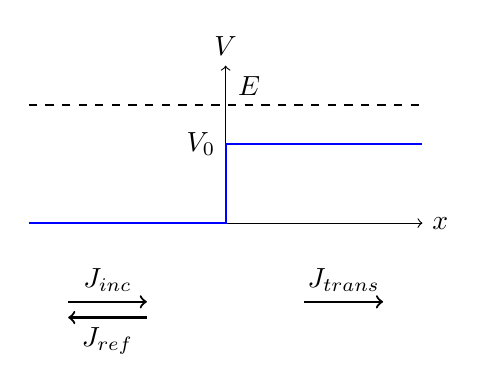
\begin{tikzpicture}
\draw[->](-2.5,0) -- (2.5,0) node[right]{$x$};
\draw[->](0,0) -- (0,2)node[above]{$V$};
\draw[blue,thick] (-2.5,0) -- (0,0) -- (0,1)node[left,black]{$V_0$} -- (2.5,1);
\draw[dashed](-2.5,1.5) -- (0,1.5) node[above,shift={(.3,0)}]{$E$} --(2.5,1.5);
\draw[->,thick](-2,-1) -- (-1,-1)node[midway,above]{$J_\rmt{inc}$};
\draw[->,thick](1,-1) -- (2,-1)node[midway,above]{$J_\rmt{trans}$};
\draw[<-,thick](-2,-1.2) -- (-1,-1.2)node[midway,below]{$J_\rmt{ref}$};
\end{tikzpicture}
\end{marginfigure}%
The wavefunction in the two regions will be described by the left-moving and right-moving waves:
\beq
\Psi(x,t) =
\begin{cases}
A\E{\I kx}\E{\I\omega t} + B\E{-\I kx}\E{\I\omega t}&x\leq 0\\
C\E{\I k'x}\E{\I\omega' t}& x>0. 
\end{cases}
\label{eq:wavefunctionfortransrefl}
\eeq
The incident traveling wave is described by the
\beq
\Psi_\rmt{inc}(x,t) = A\E{\I kx}\E{\I\omega t}
\eeq
piece with probability current
\beq
J_\rmt{inc} = \frac{\hbar k}{m}\abs{A}^2.
\eeq
Similarly, the reflected and transmitted probability currents are
\bas
J_\rmt{ref} =& -\frac{\hbar k}{m}\abs{B}^2 \\
J_\rmt{trans}=& \frac{\hbar k'}{m}\abs{C}^2.
\eas
We also want the condition that the total probability current doesn't change so that
\beq
J_\rmt{inc} = J_\rmt{ref} + J_\rmt{trans}.
\eeq
Finally, we define the {\em transmission coefficient} $T$ and the {\em reflection coefficient} $R$ as the ratio of the transmitted (and reflected) probability currents to the incoming probability current:
\beq
T \equiv \frac{\abs{J_\rmt{trans}}}{\abs{J_\rmt{inc}}} \rmt{ and } R \equiv \frac{\abs{J_\rmt{ref}}}{\abs{J_\rmt{inc}}}.
\eeq
For the simple potential barrier model, we have
\beq
T = \frac{k'}{k}\abs{\frac{C}{A}}^2 \rmt{ and } R=\abs{\frac{B}{A}}^2.
\eeq
There is one more set of conditions we need to apply: the wavefunction should be continuous and smooth (\ie the first spatial derivative is continuous) through the transition. This means that
\beq
A\E{\I\omega t} + B\E{\I\omega t} = C\E{\I\omega' t}
\eeq
and
\beq
A\I k\E{\I\omega t} - B \I k\E{\I\omega t} = C \I k'\E{\I\omega' t}. 
\eeq
From these two relationships, we can write $B$ and $C$ in terms of $A$:
\beq
B = A\frac{k - k'}{k + k'} \rmt{ and } C = A\frac{2 k}{k + k'}\E{\I(\omega - \omega')t},
\eeq\arnote[-1cm]{Fill in the missing steps. I used my \CAS.}%
giving us the transmission and reflection coefficients
\beq
T = \frac{4 k k'}{(k + k')^2}\rmt{ and } R = \left(\frac{k-k'}{k+k'}\right)^2.
\eeq
This agrees with our condition that $T + R = 1$. Furthermore, if $V_0 = 0$ then $k=k'$ and there is no reflection and there is full transmission, $T=1$. We can also write these in terms of $E$ and $V_0$:
\beq
T = \frac{4\sqrt{1-V_0/E}}{(1+\sqrt{1-V_0/E})^2}\rmt{ and } R=\left(\frac{1-\sqrt{1-V_0/E}}{1+\sqrt{1-V_0/E}}\right)^2.
\eeq
These results are shown in Figure \ref{fig:transref} and start with $T=1$, $R=0$ for no barrier, then eventually end with all reflection and no transmission when $E=V_0$.
\begin{marginfigure}
\centering
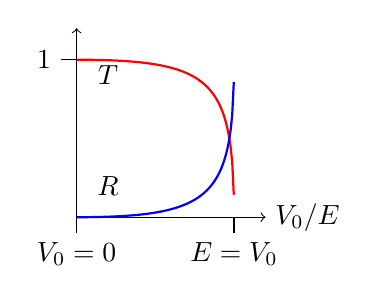
\begin{tikzpicture}[scale=2]
\draw[->] (0,0) -- (1.2,0)node[right]{$V_0/E$};
\draw[->] (0,0) -- (0,1.2);
\draw[domain=0:1,samples=100,red,thick] plot({\x},{4 * sqrt(1-\x)/((1+sqrt(1-\x))^2)});
\draw[domain=0:1,samples=100,blue,thick] plot({\x},{((1-sqrt(1-\x))^2)/((1+sqrt(1-\x))^2)});
\node at (.2,.9){$T$};
\node at (.2,.2){$R$};
\draw(0,1) -- (-.1,1)node[left]{$1$};
\draw(0,0) -- (0,-.1)node[below]{$V_0 = 0$};
\draw(1,0) -- (1,-.1)node[below]{$E = V_0$};
\end{tikzpicture}
\caption{ }
\label{fig:transref}
\end{marginfigure}


\begin{exercise}
What are the transmission and reflection coefficients if the wave is initially traveling to the left from the right and $E>V_0$?
\end{exercise}

\begin{exercise}
What are the transmission and reflection coefficients if the wave is initially traveling to the right and the initial energy is less than the potential barrier, $E<V_0$?
\end{exercise}

\section{Tunneling Barrier}
\label{tunnelingdelta}
What if, instead of a change in the potential, there was a very large, but very narrow potential barrier? This models the situation where a long thin wire has a very narrow gap in it. We model the potential as a Dirac delta-function: $V(x) = \alpha\;\delta(x)$. We have the same situation as before, but with one exception: the wavefunction is no longer smooth through $x=0$, but has a kink in it.
\begin{marginfigure}
\centering
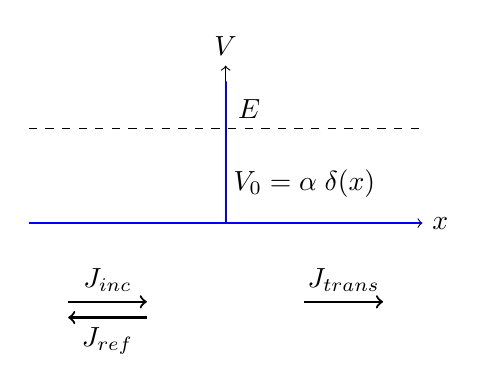
\begin{tikzpicture}
\draw[->](-2.5,0) -- (2.5,0) node[right]{$x$};
\draw[->](0,0) -- (0,2)node[above]{$V$};
\draw[blue,thick] (-2.5,0) -- (0,0) -- (0,1.8) -- (0,0) -- (2.5,0);
\node at (1,.5) {$V_0 = \alpha\;\delta(x)$};
\draw[dashed](-2.5,1.2) -- (0,1.2) node[above,shift={(.3,0)}]{$E$} --(2.5,1.2);
\draw[->,thick](-2,-1) -- (-1,-1)node[midway,above]{$J_\rmt{inc}$};
\draw[->,thick](1,-1) -- (2,-1)node[midway,above]{$J_\rmt{trans}$};
\draw[<-,thick](-2,-1.2) -- (-1,-1.2)node[midway,below]{$J_\rmt{ref}$};
\end{tikzpicture}
\end{marginfigure}%
We return to the TISWE in order to determine the effect of the delta function on the potential. We integrate over a very small interval around $x=0$ of width $2\epsilon$:
\beq
-\frac{\hbar^2}{2m}\int\displaylimits_{-\epsilon}^{\epsilon}\frac{d^2\psi}{dx^2}dx + \int\displaylimits_{-\epsilon}^{\epsilon}V(x)\psi(x)dx = E\int\displaylimits_{-\epsilon}^{\epsilon}\psi(x)dx.
\eeq\marginnote{\ref{tool:TISWE}}
The right side goes to zero as $\epsilon\rightarrow0$ so this gives us
\beq
\left.\frac{d\psi}{dx}\right|_{-\epsilon}^{\epsilon} = \frac{2m}{\hbar^2}\int\displaylimits_{-\epsilon}^{\epsilon}V(x)\psi(x)dx.
\eeq\arnote[-1cm]{There are missing steps to fill in here.}
We then use the definition of the delta function to get that the difference in the derivative on either side of the delta function is related to the wavefunction at $x=0$:
\beq
\left.\frac{d\psi}{dx}\right|_{0+} - \left.\frac{d\psi}{dx}\right|_{0-} = \frac{2m\alpha}{\hbar^2}\psi(x=0).
\label{eq:deltadifferenceatzero}
\eeq
We now apply the boundary conditions to the wavefunction from Eq.~(\ref{eq:wavefunctionfortransrefl}) where $k' = k$ since the potential is zero on both sides of $x=0$ and with the delta-function barrier to get
\beq
A + B = C
\eeq
and
\beq
C \I k- \left(A\I k - B \I k \right) = \frac{2m\alpha}{\hbar^2}C.
\eeq
The transmission and reflection coefficients (with $k=k'$) are then
\beq
T = \frac{k^2 \hbar^4}{m^2\alpha^2 + k^2 \hbar^4} \rmt{ and } R = \frac{m^2\alpha^2}{m^2\alpha^2 + k^2\hbar^4}.
\eeq\arnote[-1.2cm]{More missing steps. Use your \CAS to simplify the algebra.}
We simplify this by relating the delta-potential coefficient to an energy scale $V_0$:
\beq
\alpha \equiv \sqrt{\frac{2V_0 \hbar^2}{m}}.
\eeq\marginnote[-1.2cm]{The units for $\alpha$ are [energy$\cdot$length]. This combination gives those units.}%
The transmission and reflection coefficents are then
\beq
T = \frac{1}{V_0/E + 1} \rmt{ and } R = \frac{V_0/E}{V_0/E + 1}.
\eeq%
\begin{marginfigure}[1cm]
\centering
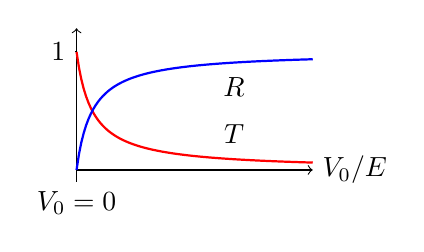
\begin{tikzpicture}[x=.2cm,y=1.5cm]
\draw[->] (0,0) -- (15,0)node[right]{$V_0/E$};
\draw[->] (0,0) -- (0,1.2);
\draw[domain=0:15,samples=100,red,thick] plot({\x},{1/(\x + 1))});
\draw[domain=0:15,samples=100,blue,thick] plot({\x},{\x/(\x + 1)});
\node at (10,.7){$R$};
\node at (10,.3){$T$};
\draw(0,1) -- (-.1,1)node[left]{$1$};
\draw(0,0) -- (0,-.1)node[below]{$V_0 = 0$};

\end{tikzpicture}
\end{marginfigure}%
So even though there would be no way for a classical system to make it though this infinitely tall barrier, the quantum MWM has a finite probability of the system tunneling through the barrier.

\begin{exercise}
What are the transmission and reflection coefficients if we model a very small {\em attractive} potential (\ie a positive defect in the wire for an electron) as a delta function $V(x) = -\alpha\;\delta(x)$?
\end{exercise}




%---------------------------------------
\chapter{Strongly Confined Systems}
\label{ch:infinitewell}

\section{1D Quantum Dot Model}

One of the simplest quantum structures we can model is the {\em quantum well}. This is a structure where a thin layer of one material is sandwiched between two layers of a different material. We'll call the thin layer Material \#1 and model it as having thickness $L$.\marginnote{In practice, this layer can be made a few tens of atoms thick using molecular beam epitaxy.}
\begin{marginfigure}
\begin{tikzpicture}

%top
\begin{scope}[canvas is xz plane at y=1.5,shift={(0,0,0)}]
\fill[black!30] (-1,-1) rectangle +(2,2);
\end{scope}

%right
\begin{scope}[canvas is yz plane at x=1]
\fill[black!40] (-.3,-1) rectangle +(.6,2);

\fill[black!60] (.3,-1) rectangle +(1.2,2);
\fill[black!60] (-1.5,-1) rectangle +(1.2,2);

\end{scope}

%front
\begin{scope}[canvas is xy plane at z=1,shift={(0,0,0)}]
\fill[black!30] (-1,-.3) rectangle +(2,.6);
\fill[black!40] (-1,.3) rectangle +(2,1.2);
\fill[black!40] (-1,-1.5) rectangle +(2,1.2);
\end{scope}

\draw[dashed](0,0,0) -- (1,0,0);
\draw[->](1,0,0) -- (2,0,0)node[right]{$y$};
\draw[dashed](0,0,0) -- (0,1.5,0);
\draw[->](0,1.5,0) -- (0,2,0)node[right]{$z$};
\draw[dashed](0,0,0) -- (0,0,1);
\draw[->](0,0,1) -- (0,0,2)node[right]{$x$};

\draw[<->](-1.2,-.3,1)--(-1.2,.3,1) node[midway,left]{$L$};

\node at (2,1,0){Material \#2};
\node at (2,-1,0){Material \#2};
\node at (2.3,0.4,0){Material \#1};

\end{tikzpicture}
\end{marginfigure}

We'll first develop a simple model of the potential for an electron in this quantum well. We'll add complexity to the model as we move forward.
\beq
V(\vec{r}) = \begin{cases}0 & \rmt{for all } x \rmt{ and } y\\
& \\
0 & \displaystyle \rmt{for } \abs{z}\leq \frac{L}{2}\\
& \\
\infty &\displaystyle \rmt{for } \abs{z} > \frac{L}{2}
\end{cases}
\eeq

We model the dynamics of the electron following our Technique \ref{tactis:TISE}. We first model the total energy as the Hamiltonian operator in 3D and we will use the positionn basis since the potential energy is dependent on position. This leads to the TISWE, Eq.~(\ref{eq:TISWE}).\marginnote{\ref{tool:TISWE}} Because our potential has the form $V(x,y,z) = V(x) + V(y) + V(z)$, we can separate out the energy eigenfunction into three variables:
\beq
\psi_E(x,y,z) = \psi_X(x)\psi_Y(y)\psi_Z(z).
\eeq
That means we have three separate wave equations:\marginnote{\ref{tool:TISWE}}%
\bas
-\frac{\hbar^2}{2m}\frac{d^2\psi_X(x)}{dx^2} = & E_x \psi_X(x) \\
-\frac{\hbar^2}{2m}\frac{d^2\psi_Y(y)}{dy^2} = & E_y \psi_Y(y) \\
-\frac{\hbar^2}{2m}\frac{d^2\psi_Z(z)}{dz^2} + V(z) \psi_Z(z) = & E_z \psi_Z(z).
\eas
The $x$ and $y$ directions are just the free MWM for the electron with solutions
\beq
\psi_X(x) =  A_x\E{\I k_x x} \rmt{ and } \psi_Y(y) =  A_y\E{\I k_y y} 
\eeq
where
\beq
k_x = \sqrt{\frac{2 m E_x}{\hbar^2}} \rmt{ and }k_y = \sqrt{\frac{2 m E_y}{\hbar^2}}.
\eeq
As before, there are no restrictions on either $k_x$ or $k_y$ and in order to make normalizable quantum states we would need to form these into a wave packet.

\subsection{Infinite Quantum Well}

We now work on the $z$-direction where
\beq
V(z) = \begin{cases}
0 & \displaystyle \rmt{for } \abs{z}\leq \frac{L}{2}\\
& \\
\infty &\displaystyle \rmt{for } \abs{z} > \frac{L}{2}.
\end{cases}
\eeq
\begin{marginfigure}[-2cm]
\centering
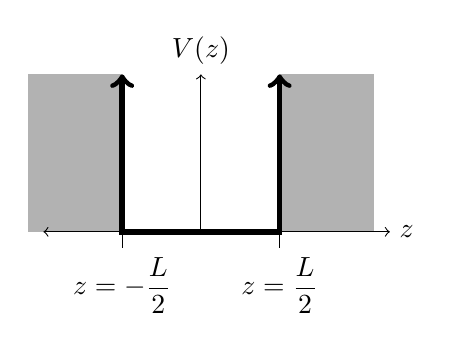
\begin{tikzpicture}
\fill[black!30] (-2.2,0) rectangle +(1.2,2);
\fill[black!30] (1,0) rectangle +(1.2,2);
\draw[<->](-2,0) -- (2.4,0)node[right]{$z$};
\draw[->](0,0) -- (0,2)node[above]{$V(z)$};

\draw[line width=2pt,<->](-1,2) -- (-1,0) -- (1,0) -- (1,2);

\draw (-1,0) -- (-1,-.2) node[below,align=center] {$\displaystyle z=-\frac{L}{2}$};
\draw (1,0) -- (1,-.2) node[below,align=center] {$\displaystyle z=\frac{L}{2}$};

\end{tikzpicture}
\end{marginfigure}

So our TISWE is now\marginnote{\ref{tool:TISWE}}%
\beq
-\frac{\hbar^2}{2m}\frac{d^2\psi_Z(z)}{dz^2} =  E_z \psi_Z(z), \qquad -\frac{L}{2}\leq z \leq \frac{L}{2}.
\label{eq:tisweinfbox}
\eeq
The solution to this second-order differential equation is a linear combination of sines and cosines
\beq
\psi_Z(z) = A \cos(k_z z) + B \sin(k_z z) \rmt{ where } k_z = \sqrt{\frac{2 m E_z}{\hbar^2}}.
\eeq
However, in order to match the boundary conditions, we must limit the allowable values for $k_z$. We are modeling the quantum well so that the electron is not allowed outside of Material \#1, so we must have
\beq
\psi_Z(z) = 0 \rmt{ for } \abs{z} > \frac{L}{2}.
\eeq
\marginnote{We also normally require that the wavefunction be smooth. The exception is at points where we model the potential as infinite. This model is only an approximation and we'll improve it later.}Finally, we require that the wavefunction be continuous which means that the value of $\psi_Z$ must be near zero near the boundaries. This means that $\psi_Z(-L/2) = \psi_Z(L/2) = 0$. The way to make this happen is to fix $k_z = n \pi z/(2L)$ where $n$ is an integer. Unfortunately we can't make this happen simultaneously with both the sine and the cosine solutions with the same $k_z$, so we have to split it up into two different types of solutions with even parity and odd parity, shown in Figure ~\ref{fig:sincos}
\beq
\psi_{Z,n}(z) = \begin{cases}
\displaystyle A_z \cos\left(\frac{n\pi z}{L}\right) &\displaystyle \abs{z}\leq\frac{L}{2},\; n = 1,3,5,\ldots\\
&\\
\displaystyle B_z \sin\left(\frac{n\pi z}{L}\right) &\displaystyle \abs{z}\leq\frac{L}{2},\; n = 2,4,6,\ldots\\
& \\
0 & \displaystyle\abs{z}>\frac{L}{2}.
\end{cases}
\label{eq:psiforinfwell}
\eeq
\begin{figure}
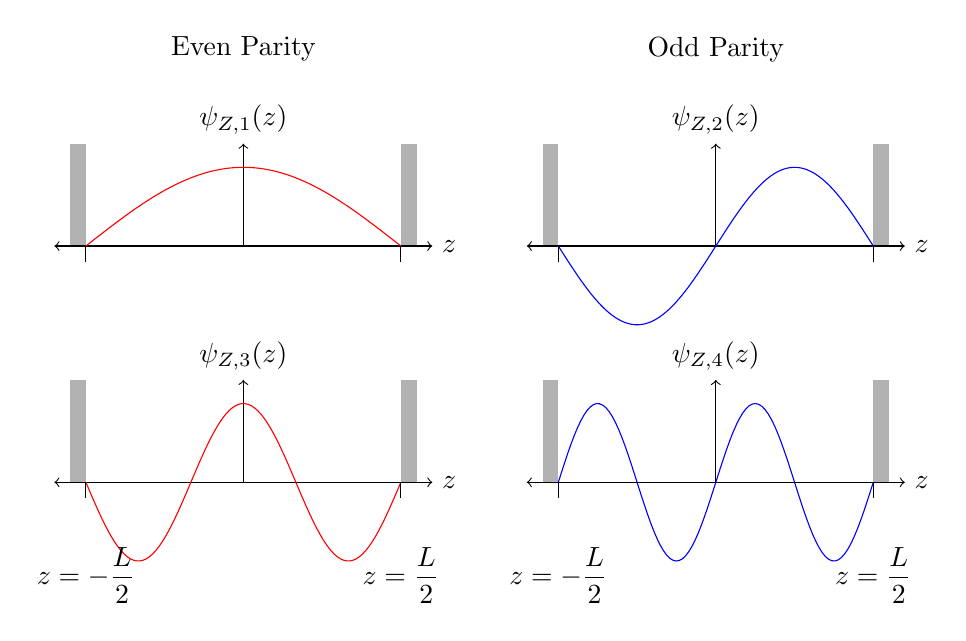
\begin{tikzpicture}
\begin{scope}[shift={(-3,3)}]
\node at (0,2.5) {Even Parity};
\fill[black!30] (-2.2,0) rectangle +(.2,1.3);
\fill[black!30] (2,0) rectangle +(.2,1.3);
\draw[<->](-2.4,0) -- (2.4,0)node[right]{$z$};
\draw[->](0,0) -- (0,1.3)node[above]{$\psi_{Z,1}(z)$};
\draw[domain=-2:2,samples=100,red] plot({\x},{cos(\x/4*180)});
\draw (-2,0) -- (-2,-.2);
\draw (2,0) -- (2,-.2);
\end{scope}

\begin{scope}[shift={(-3,0)}]
\fill[black!30] (-2.2,0) rectangle +(.2,1.3);
\fill[black!30] (2,0) rectangle +(.2,1.3);
\draw[<->](-2.4,0) -- (2.4,0)node[right]{$z$};
\draw[->](0,0) -- (0,1.3)node[above]{$\psi_{Z,3}(z)$};
\draw[domain=-2:2,samples=100,red] plot({\x},{cos(3*\x/4*180)});
\draw (-2,0) -- (-2,-.2) node[below,align=center,shift={(0,-.5)}] {$\displaystyle z=-\frac{L}{2}$};
\draw (2,0) -- (2,-.2) node[below,align=center,shift={(0,-.5)}] {$\displaystyle z=\frac{L}{2}$};
\end{scope}

\begin{scope}[shift={(3,3)}]
\node at (0,2.5) {Odd Parity};
\fill[black!30] (-2.2,0) rectangle +(.2,1.3);
\fill[black!30] (2,0) rectangle +(.2,1.3);
\draw[<->](-2.4,0) -- (2.4,0)node[right]{$z$};
\draw[->](0,0) -- (0,1.3)node[above]{$\psi_{Z,2}(z)$};
\draw[domain=-2:2,samples=100,blue] plot({\x},{sin(2*\x/4*180)});
\draw (-2,0) -- (-2,-.2);
\draw (2,0) -- (2,-.2);
\end{scope}

\begin{scope}[shift={(3,0)}]
\fill[black!30] (-2.2,0) rectangle +(.2,1.3);
\fill[black!30] (2,0) rectangle +(.2,1.3);
\draw[<->](-2.4,0) -- (2.4,0)node[right]{$z$};
\draw[->](0,0) -- (0,1.3)node[above]{$\psi_{Z,4}(z)$};
\draw[domain=-2:2,samples=100,blue] plot({\x},{sin(4*\x/4*180)});
\draw (-2,0) -- (-2,-.2) node[below,align=center,shift={(0,-.5)}] {$\displaystyle z=-\frac{L}{2}$};
\draw (2,0) -- (2,-.2) node[below,align=center,shift={(0,-.5)}] {$\displaystyle z=\frac{L}{2}$};
\end{scope}

\end{tikzpicture}
\caption[][3cm]{The first four energy eigenfunctions with even and odd parity.}
\label{fig:sincos}
\end{figure}
We now have a good idea on how to make this a general technique.

\begin{tacticsbox}
\label{tactis:TISWEBC}
To solve the time-independent Schr\"{o}dinger wave equation with boundary conditions:
\begin{enumerate}
\item Model the interaction as a time-independent Hamiltonian in a basis that makes sense given the potential.
\item Determine the TISWE for the position coordinates of the system.
\item Solve the second-order differential equation --- there should be two independent solutions.
\item Use the Boundary Conditions to limit the solutions to physically acceptable energy eigenfunctions.
\item Determine the energy eigenvalues for the eigenfunctions.
\end{enumerate}
\end{tacticsbox}

Our last step is to determine the energy eigenvalues for the eigenfunctions. In order to match the boundary conditions we had to set $k_z = n\pi/L$ where $n$ is a positive integer. That means that our energy eigenvalues are\arnote{Work out the energies.}
\beq
E_{z,n} = \frac{\hbar^2 \pi^2 n^2}{2 m L^2} \rmt{ where }n=1,2,3,\ldots
\label{eq:Eforinfwell}
\eeq
We return now to the quantum well model. The energy eigenvalues for the electron in the well are the sum of the three energies: $E = E_x + E_y + E_z$. The energies along the $x$ and $y$ directions are the free MWM energies, plus the quantized energy along the $z$-direction:
\beq
E = \frac{\hbar^2}{2m}\left(k_x^2 + k_y^2 + \frac{\pi^2 n^2}{L^2}\right), \qquad n=1,2,3,\ldots
\eeq

\begin{exercise}
What is the average momentum in the $z$-direction for an electron that is in one of the energy eigenstates in the quantum well?
\end{exercise}

\subsection{Time-dependent superposition states}
Our final step from Techique \ref{tactis:TISE} is to apply the initial conditions and determine the time evolution of the wavefunction as a sum of energy eigenfunctions. We'll do this as an example.

\begin{example}
An electron confined in a quantum well starts in an equal superposition of the first two energy eigenstates. What is the probability of measuring the $z$-position of the electron in the top half of the well as a function of time?

\model We'll model the electron as a matter wave and we'll model the quantum well as an infinte potential with thickness $L$ centered at $z=0$. Because we're only interested in the $z$-direction, we'll ignore the $x$ and $y$ wavefunctions and concentrate on the $z$ wavefunction.

\vis Our inital wavefunction is the sum of the first even and the first odd parity position wavefunctions as seen in Fig.~\ref{fig:281a}
\begin{figure}
\centering
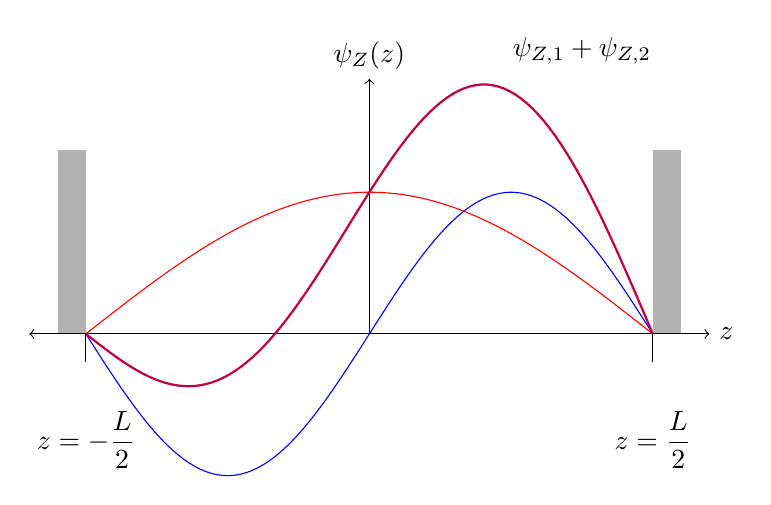
\begin{tikzpicture}[scale=1.8]

\fill[black!30] (-2.2,0) rectangle +(.2,1.3);
\fill[black!30] (2,0) rectangle +(.2,1.3);
\draw[<->](-2.4,0) -- (2.4,0)node[right]{$z$};
\draw[->](0,0) -- (0,1.8)node[above]{$\psi_{Z}(z)$};
\draw[domain=-2:2,samples=100,red] plot({\x},{cos(\x/4*180)});
\draw[domain=-2:2,samples=100,blue] plot({\x},{sin(2*\x/4*180)});
\draw[domain=-2:2,samples=100,purple,thick] plot({\x},{cos(\x/4*180) + sin(2*\x/4*180)});
\draw (-2,0) -- (-2,-.2) node[below,align=center,shift={(0,-.5)}] {$\displaystyle z=-\frac{L}{2}$};
\draw (2,0) -- (2,-.2) node[below,align=center,shift={(0,-.5)}] {$\displaystyle z=\frac{L}{2}$};
\node at (1.5,2){$\psi_{Z,1} + \psi_{Z,2}$};

\end{tikzpicture}
\caption[][2cm]{ }
\label{fig:281a}
\end{figure}

\sol We need to find the normalization constant for the initial wavefunction which is in an equal superposition of the first two energy eigenstates:
\beq
\psi_Z(z,0) = A\left[\cos\left(\frac{\pi z}{L}\right) + \sin\left(\frac{2\pi z}{L}\right)\right]
\eeq  
The normalization constraint means that\arnote{Work this normalization out on your own.}
\beq
1 = \int\displaylimits_{-L/2}^{L/2} \abs{\psi_Z(z,0)}^2dz = \abs{A}^2 L \rightarrow \; A = \sqrt{\frac{1}{L}}.
\eeq

Now the wavefunction as a function of time is
\beq
\psi_Z(z,t) = \sqrt{\frac{1}{L}}\left[\cos\left(\frac{\pi z}{L}\right)\E{-\I E_{z,1}t/\hbar}  + \sin\left(\frac{2\pi z}{L}\right)\E{-\I E_{z,2}t/\hbar}\right]
\eeq
where $E_{z,n} = \hbar^2 \pi^2 n^2/(2 m L^2)$. We can simplify this a bit by defining the angular frequency
\beq
\omega \equiv \frac{\hbar \pi^2}{2 m L^2}.
\eeq
The wavefunction is then
\beq
\psi_Z(z,t) = \sqrt{\frac{1}{L}}\left[\cos\left(\frac{\pi z}{L}\right)\E{-\I \omega t}  + \sin\left(\frac{2\pi z}{L}\right)\E{-\I 2\omega t}\right].
\eeq
We want the probability of measuring the electron in the top half of the quantum well, which we will model as $0\leq z\leq L/2$. The probability is then
\beq
P(0\leq z\leq L/2) = \int\displaylimits_{0}^{L/2} \abs{\psi_Z(z,t)}^2dz = \frac{1}{2} + \frac{4}{3\pi}\cos(\omega t).
\eeq

\assess The wavefunction units check out [1/$\sqrt{\rmt{length}}$], the angular frequency units check: 1/time. The probability starts high and then oscillates down. That makes sense as the wavefunction ``sloshes'' in the well. We see the probability increase and decrease as a function of time in Figure~\ref{fig:281b}.
\begin{marginfigure}[-2cm]
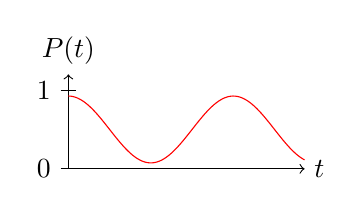
\begin{tikzpicture}
\draw[->](0,0) -- (3,0)node[right]{$t$};
\draw[->](0,0) -- (0,1.2)node[above]{$P(t)$};
\draw[domain=0:3,samples=100,red] plot({\x},{0.5 + 4/(3*3.14)*cos(3*\x*180/pi)});
\draw(-0.1,1)node[left]{$1$} -- (0.1,1);
\draw(-0.1,0)node[left]{$0$} -- (0.1,0);
\end{tikzpicture}
\caption{ }
\label{fig:281b}
\end{marginfigure}

\end{example}

\begin{exercise}
An electron confined in a quantum well starts in an equal superposition of the first two even energy eigenstates. What is the probability of measuring the $z$-position of the electron in the middle half (\ie one-quarter to three-quarters of the well thickness) of the well as a function of time? Animate the motion of the real part of the wavefunction.

\end{exercise}

\section{3D Quantum Dot Model}

We can generalize this model to describe quantum wires where the electron is confined to move along a single direction with a thin wire. We could also use the model to describe a very small volume where the electron is confined known as a {\em quantum dot}, shown in Fig. \ref{quantum dot photo}. If we model the quantum dot as a cube having lengths $L_x$, $L_y$ and $L_z$ then the energy eigenvalues are
\beq
E = \frac{\pi^2 \hbar^2}{2m}\left(\frac{n_x^2}{L_x^2}+\frac{n_y^2}{L_y^2}+\frac{n_z^2}{L_z^2}\right)
\eeq
where $n_x$, $n_y$ and $n_z$ are all positive integers.
\begin{marginfigure}
\centering
\includegraphics[width=0.6\textwidth]{QuantumDotPhoto} 
\caption{A scanning electron microscope image of quantum dots grown on a semiconductor surface.  The size of the image is 150~nm $\times$ 150~nm.  [Taken from B. J. Riel, Am. J. Phys. {\bf 76}, 750 (2008).]}
\label{quantum dot photo}
\end{marginfigure}

\section{Time-Independent Perturbation Model}
\label{sec:tipertmod}
We now want to model what happens when we have a system that starts with a Hamiltonian $\hat{H}^0$ and with known energy eigenstates $\ket{\psi_n^0}$ such that
\beq
\hat{H}^0\ket{\psi_n^0}  = E_n^0\ket{\psi_n^0}
\eeq
and then we add a small perturbation to the system. We'll model this using a small ``bump'' in the potential at the bottom of an infinite quantum well. In this case we expect the energy eigenvalues to be {\em mostly} the initial energy $E_n^0$ with a small correction. We model the modified Hamiltonaian as the operator
\beq
\hat{H}\ket{\psi_n}  = E_n\ket{\psi_n} \rmt{ where }\hat{H} \equiv \hat{H}^0 + \lambda \hat{H}'
\label{eq:pertham}
\eeq
for a small parameter $\lambda$.
\begin{marginfigure}[-2cm]
\centering
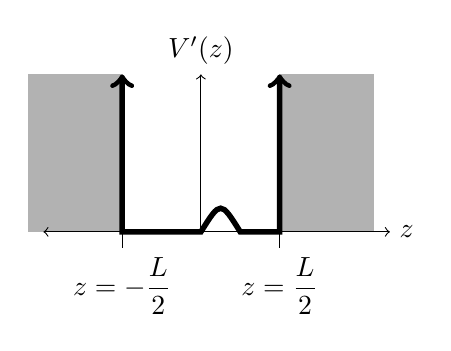
\begin{tikzpicture}
\fill[black!30] (-2.2,0) rectangle +(1.2,2);
\fill[black!30] (1,0) rectangle +(1.2,2);
\draw[<->](-2,0) -- (2.4,0)node[right]{$z$};
\draw[->](0,0) -- (0,2)node[above]{$V'(z)$};

\draw[line width=2pt,<->](-1,2) -- (-1,0) -- (0,0) ..controls(0.25,0.4) .. (0.5,0) --(1,0) -- (1,2);

\draw (-1,0) -- (-1,-.2) node[below,align=center] {$\displaystyle z=-\frac{L}{2}$};
\draw (1,0) -- (1,-.2) node[below,align=center] {$\displaystyle z=\frac{L}{2}$};

\end{tikzpicture}
\end{marginfigure}
We expand the eigenstates of this new operator $\hat{H}$ as a power series expansion in the small parameter $\lambda$. So our model has the eigenstates as mostly the original eigenstates with a small correction $\ket{\psi_n^1}$ and even smaller corrections that we will mostly ignore:
\beq
\ket{\psi_n}\approx \ket{\psi_n^0} + \lambda \ket{\psi_n^1} + \lambda^2 \ket{\psi_n^2} + \ldots.
\eeq
In this case the energy eigenvalues would be
\beq
E_n \approx E_n^0 + \lambda E_n^1 + \lambda^2 E_n^2 + \ldots
\eeq
where again, the first term is the unpertrubed energy and $E_n^1$ is the first-order correction, and so forth. We now insert these into Eq.~(\ref{eq:pertham}), expand, and keep only the terms with no $\lambda$ or a single power of $\lambda$ in them.\arnote{Work out the expansion.} That gives us
\beq
\lambda\left(\hat{H}^0\ket{\psi_n^1} + \hat{H}'\ket{\psi_n^0}\right) = \lambda\left(E_n^0\ket{\psi_n^1} + E_n^1\ket{\psi_n^0} \right).
\eeq
We multiply both sides by $\bra{\psi_n^0}$ and get the first-order correction to the energy eigenvalue
\beq
E_n^1 = \bra{\psi_n^0}\hat{H}'\ket{\psi_n^0}.
\label{eq:energyperturbation}
\eeq
This means if we know the unperturbed eigenstates and the changes to the Hamiltonian, we can model how these changes will shift the energy of the system. \marginnote[-2cm]{Finding the first-order correction to the eigenstates will be an exercise, but they aren't as useful for us as the energies.} In the end we'll assume that $\lambda = 1$ because the perturbed Hamiltonian and the energy correction will both be very small. The final energies will be
\beq
E_n = E_n^0 + E_n^1.
\eeq
\begin{example}
What is the first-order correction to the infinite quantum well energies for the odd-parity states if the left half of the well is raised by a small amount $V_0$?

\model We model the unperturbed infinite quantum well using the energy eigenstates we found before. We'll model this change as a small perturbation and use the time-independent perturbation model to find the energy shift. The perturbed Hamiltonian is just a constant $V_0$ over the interval of $-L/2 \leq z \leq 0$.

\vis Our quantum well now looks like Figure~\ref{fig:ex282a}.

\begin{figure}
\centering
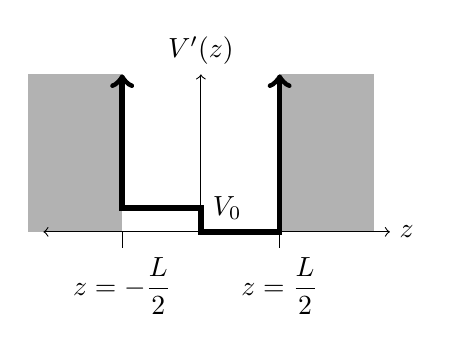
\begin{tikzpicture}
\fill[black!30] (-2.2,0) rectangle +(1.2,2);
\fill[black!30] (1,0) rectangle +(1.2,2);
\draw[<->](-2,0) -- (2.4,0)node[right]{$z$};
\draw[->](0,0) -- (0,2)node[above]{$V'(z)$};

\draw[line width=2pt,<->](-1,2) -- (-1,.3) -- (0,.3) node[right]{$V_0$} -- (0,0)   --(1,0) -- (1,2);

\draw (-1,0) -- (-1,-.2) node[below,align=center] {$\displaystyle z=-\frac{L}{2}$};
\draw (1,0) -- (1,-.2) node[below,align=center] {$\displaystyle z=\frac{L}{2}$};

\end{tikzpicture}
\caption[][2cm]{ }
\label{fig:ex282a}
\end{figure}

\sol We first need normalized odd-parity eignefunctions of the unperturbed system. These are
\beq
\psi_n(z) = B_z \sin\left(\frac{n\pi z}{L}\right)\qquad \abs{z}\leq\frac{L}{2},\; n = 2,4,6,\ldots
\eeq
The normalization condition gives us that $B_z = \sqrt{2/L}$. So we find the first-order correction to the energy is 
\bas
E_n^1 = & \bra{\psi_n^0}\hat{H}'\ket{\psi_n^0} =  \int\displaylimits_{-L/2}^{0}V_0 \abs{\psi_n(z)}^2dz \\
=& \frac{V_0}{2}.
\eas

\assess This first-order correction makes sense for the odd-parity states- one half of the state will be lifted up by the energy $V_0$. However, this is only the first-order correction and we would probably find that there are other, higher-order corrections, too.

\end{example}


\begin{exercise}
Use the completeness relationship to show that the first-order correction to the eigenstates is
\beq
\ket{\psi_n^1} = \sum_{m\neq n}\frac{\bra{\psi_m^0}\hat{H}'\ket{\psi_n^0}}{E_n^0 - E_m^0}\ket{\psi_m^0}.
\eeq
\end{exercise}

\begin{exercise}
What is the first-order correction to the allowed energies in a quantum well if we model a defect in the center of the material as a delta-function
\beq
\bra{z}\hat{H}'\ket{z} = \alpha \;\delta(z)\rmt{?}
\eeq

\end{exercise}




%---------------------------------------
\chapter{Transitions Between States}


By itself, each energy eigenstate isn't all that interesting --- we know from classical mechanics that a single energy level is not what matters; it is the transition between energy levels that is physically interesting. So we now build a model that describes how a quantum state can make the transition between allowed energy eigenstates of a bound system like the infinite quantum well. This model will also work for other bound states as we'll see later.

We will focus on two energy eigenstates of the unperturbed Hamiltonian and call them $\ket{\psi_a}$ and $\ket{\psi_b}$ such that
\beq
\hat{H}^0\ket{\psi_a} = E_a \ket{\psi_a} \rmt{ and } \hat{H}^0\ket{\psi_b} = E_b \ket{\psi_b} \rmt{ where } \avg{\psi_a|\psi_b} = \delta_{ab}.
\eeq%
\begin{marginfigure}
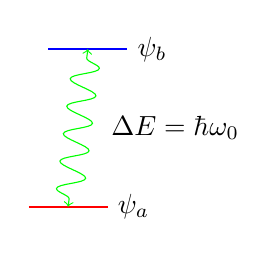
\begin{tikzpicture}
\draw[thick,red] (0,0) -- (1,0)node[right,black]{$\ket{\psi_a}$};
\draw[thick,blue] (0.25,2) -- (1.25,2)node[right,black]{$\ket{\psi_b}$};
\draw[green,<->,decorate, decoration={snake,amplitude=5,segment length=10, post length=.1cm, pre length=.1cm}](0.5,0)--(.75,2) node[midway, right,shift=({0.3,0}),black]{$\Delta E = \hbar \omega_0$};
\end{tikzpicture}
\end{marginfigure}%
We will also model the energy difference as $E_b - E_a \equiv \Delta E = \hbar \omega_0$ where $\omega_0$ is an angular frequency.

We describe an arbitrary superposition of these two energy eigenstates, as a function of time, using Eq.~(\ref{eq:soltoTDSE}):
\beq
\ket{\Psi(t)} = c_a \E{-\I E_a t/\hbar}\ket{\psi_a} +c_b \E{-\I E_b t/\hbar}\ket{\psi_b}
\label{eq:psittrans}
\eeq
where $c_a$ and $c_b$ are the complex coefficients that model the relative population of the two different eigenstates. These coefficients could potentially depend on time, so we'll keep that in mind as we look at the time evolution of the quantum state.

\section{Time-dependent Perturbation Model}
We now perturb the system as we did in Section \ref{sec:tipertmod}, but this time we are going to make the perturbation dependent on time. We are also only going to keep first-order terms, so we'll set $\lambda = 1$. The modified Hamiltonian operator is now
\beq
\hat{H} = \hat{H}^0 + \hat{H}'(t).
\eeq
We now look at the Schr\"{o}dinger equation:\marginnote{\ref{tool:sch}}% 
\beq
\I\hbar \frac{\partial \ket{\Psi(t)}}{\partial t} = \hat{H}\ket{\Psi(t)} = \hat{H}^0 \ket{\Psi(t)}+ \hat{H}'(t)\ket{\Psi(t)}.
\eeq
Because we have the explicit form of $\ket{\Psi(t)}$, Eq.~(\ref{eq:psittrans}), we can take the time derivative:\arnote[1cm]{Work out the derivative on your own.}%
\bas
\I\hbar \frac{\partial \ket{\Psi(t)}}{\partial t} = & \I\hbar \frac{\partial}{\partial t} \left(c_a \E{-\I E_a t/\hbar}\ket{\psi_a} +c_b \E{-\I E_b t/\hbar}\ket{\psi_b} \right) \\
= & E_a c_a \E{-\I E_a t/\hbar}\ket{\psi_a} + E_b c_b \E{-\I E_b t/\hbar}\ket{\psi_b} + \nonumber\\
& \I\hbar\left( \dot{c}_a \E{-\I E_a t/\hbar}\ket{\psi_a} + \dot{c}_b \E{-\I E_b t/\hbar}\ket{\psi_b} \right)
\eas
where $\dot{c}_a \equiv dc_a/dt$ and the same for $\dot{c}_b$. The first half of this is just $\hat{H}^0\ket{\Psi}$. So combining this with the Schr\"{o}dinger equation and canceling the same terms on both sides, we get
\begin{multline}
 c_a  \E{-\I E_a t/\hbar} \hat{H}' \ket{\psi_a} +  c_b \E{-\I E_b t/\hbar} \hat{H}' \ket{\psi_b} = \\ \I\hbar\left( \dot{c}_a \E{-\I E_a t/\hbar}\ket{\psi_a} + \dot{c}_b \E{-\I E_b t/\hbar}\ket{\psi_b} \right).
 \label{eq:timedepop}
\end{multline}
We will multiply both sides of this by $\bra{\psi_a}$ and repeat the same process multiplying by $\bra{\psi_b}$. We define the matrix elements of $\hat{H}'$ in the $\ket{\psi_j}$ basis as
\beq
H'_{jk} = \bra{\psi_j}\hat{H}'\ket{\psi_k}.
\label{eq:perthammatelem}
\eeq
That means that, after projecting onto Eq.~(\ref{eq:timedepop}), we get two differential equations for the amplitudes:\arnote[1cm]{Work these out in your notes.}%
\beq
\label{eq:messyceqn}
\begin{split}
\dot{c}_a =& -\frac{\I}{\hbar}\left[c_a H'_{aa} + c_b H'_{ab} \E{-\I(E_b - E_a)t/\hbar} \right]\\
\dot{c}_b =&  -\frac{\I}{\hbar}\left[c_b H'_{bb} + c_a H'_{ba} \E{\I(E_b - E_a)t/\hbar} \right].
\end{split}
\eeq
We now make a simplifying assumption: we are not interested in perturbations to the system that do anything to a single state. In other words we want $H'_{jj} = 0$. This models situations where the perturbation only couples states without shifting the states themselves.\marginnote[-1cm]{This approximation work reasonably well, though there are situations where it breaks down. The AC Stark shift is one of them.} With this approximation, Eq.~(\ref{eq:messyceqn}) becomes
\beq
\label{eq:simpceqn}
\begin{split}
\dot{c}_a =& -\frac{\I}{\hbar} c_b H'_{ab} \E{-\I\omega_0 t} \\
\dot{c}_b =&  -\frac{\I}{\hbar} c_a H'_{ba} \E{\I\omega_0 t}
\end{split}
\eeq
where we used the energy difference $\Delta E = \hbar \omega_0$ that we defined earlier. In order to say anything more about the transitions between these two states, we need to know more about the perturbation to the Hamiltonian.

\section{Dipole Transitions}
\label{sec:dipoletrans}
We focus our interaction model on an electron bound in a quantum well. We perturb the electron by sending in an ElMaW. The primary interaction between the ElMaW and the electron is due to the electric field of the wave. We model the wave as polarized in the $z$-direction and as having an approximately constant electric field magnitude that oscillates in time with angular frequency $\omega$:
\beq
E_z = E_0 \cos(\omega t).
\eeq
The potential energy of a single electron with charge $-e$ in this uniform electric field is $V(z) = -e E_z z$. We model this as the perturbed Hamilonian operator in the position basis
\beq
\hat{H}' = -e E_0 \hat{Z} \cos(\omega t). 
\eeq
We can now find the matrix elements for the perturbed Hamiltonian, Eq.~(\ref{eq:perthammatelem})
\beq
H'_{jk} = \bra{\psi_j}\hat{H}'\ket{\psi_k} = \underbrace{e\bra{\psi_j}\hat{Z}\ket{\psi_k}}_{\displaystyle \rmt{A dipole } \vec{p} = q\vec{d}}\left(-E_0\cos\omega t\right).
\label{eq:hjkdipole}
\eeq
Because the matrix element has the form of an electric dipole, these transitions are called {\em electric dipole transitions}.\marginnote[-1cm]{There are other transitions like electric quadrupole, magnetic dipole, etc.} For simplicity, we define a dipole energy 
\beq
V_{jk} \equiv - e\bra{\psi_j}\hat{Z}\ket{\psi_k} E_0 = -p E_0
\eeq
so the Hamiltonian matrix elements can now  be written
\beq
H'_{jk} = \frac{V_{jk}}{2}\left(\E{\I\omega t} + \E{-\I\omega t}\right),
\label{eq:hammatdipole}
\eeq
where we have also expanded the cosine in terms of the exponentials. 

\begin{example}
\label{ex:dipoletrans}
What are the dipole energy matrix elements for an electron in a quantum well between the first two energy eigenstates?

\model We model the electron (charge $-e$) as a quantum state in an infinite well with energy eigenfunctions given by Eq.~(\ref{eq:psiforinfwell}) and energies by Eq.~(\ref{eq:Eforinfwell}). We'll model the well as having thickness $L$. We'll also model the transition as coming from a $z$-polarized ElMaW with amplitude $E_0$.

\vis We are looking for a transition between the two energy states $E_{z,1}$ and $E_{z,2}$, shown if Figure~\ref{fig:e12psi}.

\begin{figure}
\centering
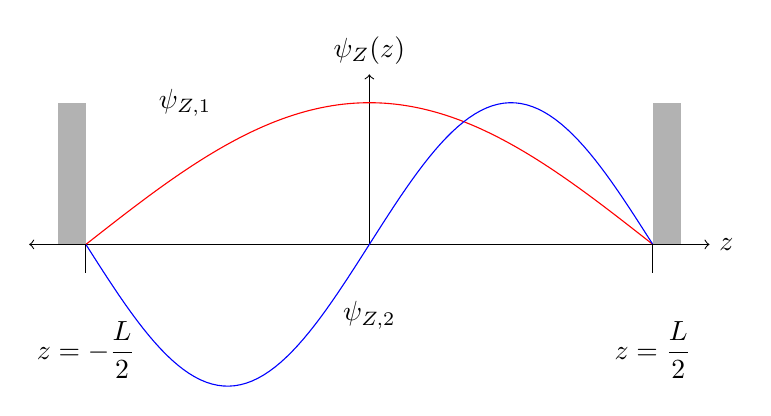
\begin{tikzpicture}[scale=1.8]

\fill[black!30] (-2.2,0) rectangle +(.2,1);
\fill[black!30] (2,0) rectangle +(.2,1);
\draw[<->](-2.4,0) -- (2.4,0)node[right]{$z$};
\draw[->](0,0) -- (0,1.2)node[above]{$\psi_{Z}(z)$};
\draw[domain=-2:2,samples=100,red] plot({\x},{cos(\x/4*180)});
\draw[domain=-2:2,samples=100,blue] plot({\x},{sin(2*\x/4*180)});
\draw (-2,0) -- (-2,-.2) node[below,align=center,shift={(0,-.5)}] {$\displaystyle z=-\frac{L}{2}$};
\draw (2,0) -- (2,-.2) node[below,align=center,shift={(0,-.5)}] {$\displaystyle z=\frac{L}{2}$};
\node at (-1.3,1){$\psi_{Z,1}$};
\node at (0,-0.5){$\psi_{Z,2}$};
\end{tikzpicture}
\caption[][1cm]{The first two energy eigenstates of the infinite quantum well.}
\label{fig:e12psi}
\end{figure}

\sol We want the dipole matrix elements $V_{12} = - e\bra{\psi_{Z,1}}\hat{Z}\ket{\psi_{Z,2}} E_0$. We need to get the normalization constants for these two eigenstates before we can find the matrix elements:

\bas
\avg{\psi_{Z,1}|\psi_{Z,1}} = & \abs{A_Z}^2 \frac{L}{2} \rightarrow \psi_{Z,1}(z) = \sqrt{\frac{2}{L}}\cos\left(\frac{\pi z}{L}\right) \\
\avg{\psi_{Z,2}|\psi_{Z,2}} = & \abs{B_Z}^2 \frac{L}{2} \rightarrow \psi_{Z,2}(z) = \sqrt{\frac{2}{L}}\sin\left(\frac{2\pi z}{L}\right)
\eas

We expand the matrix elements in the position basis:\arnote[2cm]{Work out the integrals.}%
\bas
\bra{\psi_{Z,1}}\hat{Z}\ket{\psi_{Z,2}} = &  \frac{2}{L} \int\displaylimits_{-L/2}^{L/2} \cos\left(\frac{\pi z}{L}\right) \;z\;\sin\left(\frac{2\pi z}{L}\right)dz\\
= & \frac{16 L}{9 \pi^2}.
\eas
Since this integral is symmetric, $V_{12}=V_{21}$. The dipole matrix elements are
\beq
V_{12}=V_{21} = - e E_0\frac{16 L}{9 \pi^2}.
\eeq

\assess The dipole matrix elements have units energy, so we're good there. Just to check, we tried $\bra{\psi_{Z,1}}\hat{Z}\ket{\psi_{Z,1}} =0$ which means that the dipole electric field does not couple the ground state to itself, at least not in this model.

\end{example}


We are ready to return to Eq.~(\ref{eq:simpceqn}) and insert Eq.~(\ref{eq:hammatdipole}):
\beq
\begin{split}
\dot{c}_a =& -\frac{\I V_{ab}}{2\hbar} c_b  \E{-\I\omega_0 t}\left(\E{\I\omega t} + \E{-\I\omega t}\right) \\
\dot{c}_b =&  -\frac{\I V_{ba}}{2\hbar} c_a  \E{\I\omega_0 t}\left(\E{\I\omega t} + \E{-\I\omega t}\right).
\end{split}
\label{eq:preRWA}
\eeq
Each of these differential equations has two different sets of exponential terms, one where the two angular frequencies add, and one where they are subtracted:
\beq
\E{\I(\omega + \omega_0)t} \rmt{ and } \E{\I(\omega - \omega_0)t}.
\eeq
We model the terms where the angular frequencies add as being much smaller than the other:
\beq
\E{\I(\omega + \omega_0)t} \ll \E{\I(\omega - \omega_0)t}.
\eeq
because, when we look at the time average of both of these over one period, the higher-frequency term gives an average that approaches zero. We thus approximate any term with the sum of the two angular frequencies as zero $\E{\I(\omega + \omega_0)t}\approx 0$. This is called the {\em Rotating Wave Approximation}.

\begin{exercise}
Show that the Rotating Wave Approximation works in the following situation:
\bas
\frac{d f}{dt} =& \E{\I(\omega + \omega_0)t}\\
\frac{d g}{dt} =& \E{\I(\omega - \omega_0)t}.
\eas
Show that $\abs{f} \ll \abs{g}$.

\end{exercise}

\subsection{Resonant Transitions}
We will model the incoming ElMaW as having the the same angular frequency as that associated with the energy difference between the two quantum states in our infinite well which is known as having the transition on {\em resonance}:
\beq
\omega = \omega_0.
\eeq
We now apply the Rotating Wave Approximation to Eq.~(\ref{eq:preRWA}) along with the resonance condition to get the two coupled differential equations\arnote{Run through both the approximation and the resonant condition to get here.}%
\beq
\begin{split}
\dot{c}_a =& -\frac{\I V_{ab}}{2\hbar} c_b  \\
\dot{c}_b =&  -\frac{\I V_{ba}}{2\hbar} c_a .
\end{split}
\label{eq:RWAresonance}
\eeq
We define the {\em Rabi frequency} $\Omega_0 \equiv V_{ab}/(2\hbar)$, \marginnote{Because $\Omega_0$ depends on the applied ElMaW electric field amplitude, it is an adjustable experimental parameter by changing the ElMaW intensity, Eq.~(\ref{eq:CEWAMInt}).}noting that, for our states in the infinite quantum well, the matrix elements are symmetric: $ V_{ab} =  V_{ba}$. These two coupled differential equations have solutions
\beq
\begin{split}
c_a(t) =& A \cos(\Omega_0t)  + \I B \sin(\Omega_0t)  \\
c_b(t) =&  B \cos(\Omega_0t)  + \I A \sin(\Omega_0t)  .
\end{split}
\label{eq:RWAsol}
\eeq
We need to normalize these since our initial state $\ket{\Psi(t)}$, Eq.~(\ref{eq:psittrans}) was normalized. That means that\arnote[1cm]{Work this out, too.}
\beq
\avg{\Psi(t)|\Psi(t)} = \abs{A}^2 + \abs{B}^2 = 1.
\eeq
Finally, we set the initial conditions so that
\beq
c_a(0) = A \rmt{ and } c_b(0) = B \qquad \left(\abs{c_a(0)}^2 + \abs{c_b(0)}^2 = 1\right)
\eeq
which give us
\beq
\begin{split}
c_a(t) =& c_a(0) \cos(\Omega_0t)  + \I c_b(0) \sin(\Omega_0t)  \\
c_b(t) =&  c_b(0) \cos(\Omega_0t)  + \I c_a(0) \sin(\Omega_0t).
\end{split}
\label{eq:RWAsolnorm}
\eeq

\begin{exercise}
\label{ex:elecrabi}
What is the Rabi frequency for an ElMaW with intensity $10$~$\mu$W/m$^2$ which is on-resonant between the first two energy eigenstates for an electron in a $10$~nm thick quantum well?

\end{exercise}

\section{Rabi Oscillations}
We now look at transitions between states using the on-resonance amplitude equations, Eq.~(\ref{eq:RWAsolnorm}). We model our system as starting in the lower energy eigenstate $\ket{\psi_a}$ so that $c_a(0) =1$ and $c_b(0)=0$. The time evolution of the state is now
\beq
\ket{\Psi(t)} = \cos(\Omega_0 t) \E{-\I E_a t/\hbar}\ket{\psi_a} + \I\sin(\Omega_0 t) \E{-\I E_b t/\hbar}\ket{\psi_b}.
\eeq
What is the probability of measuring the state in eigenstate $\ket{\psi_a}$? \marginnote[1cm]{\ref{tool:prob}}%
\beq
P(\ket{\psi_a}) = \abs{\avg{\ket{\psi_a|\Psi(t)}}}^2 = \cos^2(\Omega_0 t).
\eeq
Similarly, the probability of measuring the state in $\ket{\psi_b}$ is $P(\ket{\psi_b}) = \sin^2(\Omega_0 t)$. Thus the probability of measuring the two different states oscillates back and forth between them.
\begin{marginfigure}
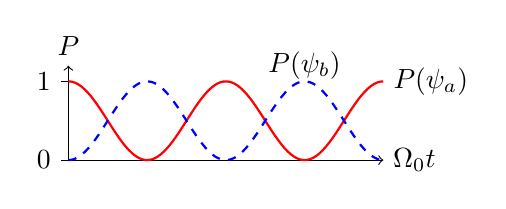
\begin{tikzpicture}
\draw[->](0,0) -- (4,0)node[right]{$\Omega_0 t$};
\draw[->](0,0) -- (0,1.2)node[above]{$P$};
\draw[domain=0:4,samples=100,red,thick] plot({\x},{(cos(\x/2*180))^2}) node[right,black]  {$P(\ket{\psi_a})$};
\draw[domain=0:4,samples=100,blue,dashed,thick] plot({\x},{(sin(\x/2*180))^2});
\node[black] at (3,1.2) {$P(\ket{\psi_b})$};
\draw(0,1) -- (-0.1,1)node[left]{$1$};
\draw(0,0) -- (-0.1,0)node[left]{$0$};
\end{tikzpicture}
\end{marginfigure}

\begin{exercise}
The same electron as in Exercise \ref{ex:elecrabi} starts in a superposition state
\beq
\ket{\Psi(0)} = \frac{1}{\sqrt{3}} \ket{\psi_{Z,1}} + \sqrt{\frac{2}{3}} \ket{\psi_{Z,2}}.
\eeq
At what time will the probability of measuring the state in $P(\ket{\psi_{Z,2}}) =1 $? Graph the probabilities of measuring both states as a function of time.
\end{exercise}

\section{Oscillator Strength}

We can also model a unitless parameter that describes the relative strength of different possible transitions. This parameter, known as the {\em oscillator strength}, gives us a quick reference as to how likely we could make transition between two energy eigenstates. The oscillator strength for an electron mass $m_e$ coupling states $\ket{\psi_a}$ and $\ket{\psi_b}$ with a $z$-polarized ElMaW is
\beq
f_{ab} = \frac{2}{3} \frac{m_e}{\hbar^2}\left|E_a - E_b\right|\abs{\bra{\psi_a}\hat{Z}\ket{\psi_b}}^2.
\label{eq:oscstr}
\eeq
The oscillator strength is unitless and is typically on a scale from $0$ to $1$. 

\begin{example}
What is the oscillator strength for the transition from Example \ref{ex:dipoletrans}?

\model Our model is the same as before - an  electron (charge $-e$, mass $m_e$) as a quantum state in an infinite well with energy eigenfunctions given by Eq.~(\ref{eq:psiforinfwell}) and energies by Eq.~(\ref{eq:Eforinfwell}). We'll model the well as having thickness $L$. We'll also model the transition as coming from a $z$-polarized ElMaW with amplitude $E_0$.

\vis The same picture as before, Fig.~\ref{fig:e12psi}, describes this situation.

\sol The oscillator strength is

\bas
f_{21} = & \frac{2}{3} \frac{m_e}{\hbar^2}\left|E_2 - E_1\right|\abs{\bra{\psi_2}\hat{Z}\ket{\psi_1}}^2 \\
=& \frac{2}{3} \frac{m_e}{\hbar^2} \left(\frac{4 \pi^2 \hbar^2}{2 m_e L^2} - \frac{\pi^2 \hbar^2}{2 m_e L^2} \right)\left[ \frac{2}{L} \int\displaylimits_{-L/2}^{L/2} \cos\left(\frac{\pi z}{L}\right) \;z\;\sin\left(\frac{2\pi z}{L}\right)dz \right]^2\\
= & \frac{2}{3} \frac{m_e}{\hbar^2} \frac{3 \pi^2 \hbar^2}{2 m_e L^2}  \left(\frac{16 L}{9 \pi^2}\right)^2 \\
= & \frac{256}{81\pi^2} \approx 0.32.
\eas

\assess Our oscillator strength is unitless and lies between $0$ and $1$ --- it isn't a very strong transition.

\end{example}


\begin{exercise}

What is the oscillator strength for transitions between
\begin{itemize}
\item[(a)] Any even parity and any odd parity states
\item[(b)] Any even parity and any other even parity states
\item[(c)] Any odd parity and any other odd parity states
\end{itemize}
of the infinite quantum well?
\end{exercise}



%---------------------------------------
\chapter{Finite Confinement}

The model we built in Chapter \ref{ch:infinitewell} was a good start to describing an electron in a quantum well, but it was only a crude approximation, since we modeled the potential difference between layers as inifinite. We now improve this model by modeling a {\em finite} potential well. We'll use the same picture: an electron is confined to a thin material (thickness $L$) in one dimension. We will again focus on the $z$-direction, recognizing that the electron is modeled by a free matter wave in the other two directions.%
%
\begin{marginfigure}
\begin{tikzpicture}

%top
\begin{scope}[canvas is xz plane at y=1.5,shift={(0,0,0)}]
\fill[black!30] (-1,-1) rectangle +(2,2);
\end{scope}

%right
\begin{scope}[canvas is yz plane at x=1]
\fill[black!40] (-.3,-1) rectangle +(.6,2);

\fill[black!60] (.3,-1) rectangle +(1.2,2);
\fill[black!60] (-1.5,-1) rectangle +(1.2,2);

\end{scope}

%front
\begin{scope}[canvas is xy plane at z=1,shift={(0,0,0)}]
\fill[black!30] (-1,-.3) rectangle +(2,.6);
\fill[black!40] (-1,.3) rectangle +(2,1.2);
\fill[black!40] (-1,-1.5) rectangle +(2,1.2);
\end{scope}

\draw[dashed](0,0,0) -- (1,0,0);
\draw[->](1,0,0) -- (2,0,0)node[right]{$y$};
\draw[dashed](0,0,0) -- (0,1.5,0);
\draw[->](0,1.5,0) -- (0,2,0)node[right]{$z$};
\draw[dashed](0,0,0) -- (0,0,1);
\draw[->](0,0,1) -- (0,0,2)node[right]{$x$};

\draw[<->](-1.2,-.3,1)--(-1.2,.3,1) node[midway,left]{$L$};

\node at (2,1,0){Material \#2};
\node at (2,-1,0){Material \#2};
\node at (2.3,0.4,0){Material \#1};

\end{tikzpicture}
\end{marginfigure}
%
We model the potential in the $z$-direction as
\beq
V(z) = \begin{cases}
0 & \displaystyle \rmt{for } \abs{z}\leq \frac{L}{2}\\
& \\
V_0 &\displaystyle \rmt{for } \abs{z} > \frac{L}{2}.
\end{cases}
\eeq
We are interested in situations where our quantum state has total energy $E<V_0$ so that the electron is bound in the quantum well. We use the scattering techniques from Chapter~\ref{ch:scattering} to treat that situation.\marginnote{If $E>V_0$ we have to treat the well as a scattering problem of a matter wave from a defect.} This model naturally divides itself into three zones, shown in Figure \ref{fig:finitewell}.
\begin{figure}
\centering
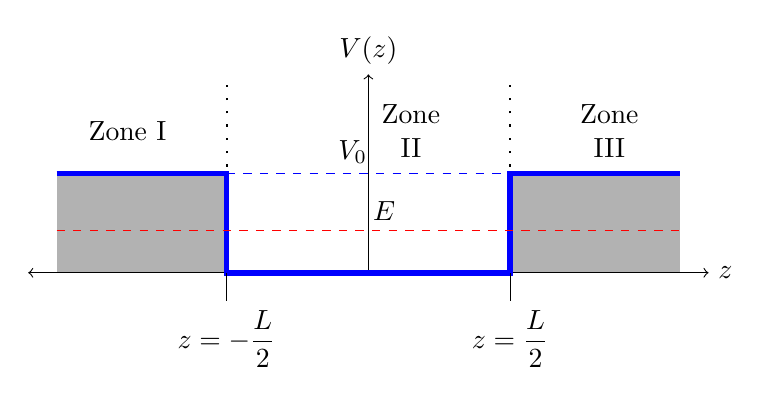
\begin{tikzpicture}[scale=1.8]

\fill[black!30] (-2.2,0) rectangle +(1.2,.7);
\fill[black!30] (1,0) rectangle +(1.2,.7);
\draw[<->](-2.4,0) -- (2.4,0)node[right]{$z$};
\draw[->](0,0) -- (0,1.4)node[above]{$V(z)$};

\draw[loosely dotted,thick] (-1,0) -- (-1,1.4);
\draw[loosely dotted,thick] (1,0) -- (1,1.4);

\draw[line width=2pt,blue](-2.2,.7) -- (-1,.7) -- (-1,0) -- (1,0) -- (1,.7) -- (2.2,.7);
\draw (-1,0) -- (-1,-.2) node[below,align=center,shift={(0,0)}] {$\displaystyle z=-\frac{L}{2}$};
\draw (1,0) -- (1,-.2) node[below,align=center,shift={(0,0)}] {$\displaystyle z=\frac{L}{2}$};
\node[text width=1cm,align=center] at (-1.7,1){Zone I};

\node[text width=1cm,align=center] at (.3,1){Zone II};
\node[text width=1cm,align=center] at (1.7,1){Zone III};
\draw[dashed,red](-2.2,.3) -- (2.2,.3) node[midway,above,black,shift={(.2,0)}]{$E$};

\draw[dashed,blue](-1,.7) -- (1,.7) node[midway,above,black,shift={(-.2,0)}]{$V_0$};

\end{tikzpicture}
\caption[][1cm]{The finite potential model for an electron in a quantum well.}
\label{fig:finitewell}
\end{figure}
%

We follow the Technique \ref{tactis:TISWEBC}. It makes sense to work in the $z$-basis in describing our Hamiltonian as we have a potential that depends on $z$:\marginnote{\ref{tool:sch}}%
\beq
\bra{z}\left(\I\hbar\frac{\partial}{\partial t}\ket{\Psi} = \hat{H}\ket{\Psi}\right).
\eeq
We need the TISWE in this basis. We actually have two different TISWEs depending on whether we are in zone II or in zones I and III. We'll start in zone II.

\subsection{TISWE in Zone II}
In this zone we have the case where $E>V_0$, so our TISWE in the $z$ basis is\marginnote{\ref{tool:TISWE}}%
\beq
\begin{split}
-\frac{\hbar^2}{2m}\frac{d^2\psi(z)}{dz^2} + V(z) \psi(z) = E \psi(z) \;\rightarrow\; \\ \frac{d^2\psi^\rmt{II}(z)}{dz^2} = -\frac{2m}{\hbar^2}E \psi^\rmt{II}(z),
\label{eq:TISWEzone2}
\end{split}
\eeq%
since $V_0 = 0$ in this zone. We define the real, positive wave number
\beq
k^2 \equiv \frac{2m E}{\hbar^2}
\eeq
so the TISWE becomes
\beq
\frac{d^2\psi^\rmt{II}(z)}{dz^2} = -k^2 \psi^\rmt{II}(z).
\eeq
This has solutions that can be written as a sum of sines and cosines (even an odd parity solutions again): $\psi^\rmt{II}(z) = A \cos kz + B \sin kz$ where $A$ and $B$ are constants. Before we can apply the boundary conditions and initial conditions, we need to take care of the other two zones.

\subsection{TISWE in Zones I and III}
If this were a classical model, we wouldn't have to worry about these zones at all--- there is no way in the particle model for a particle to get to the shaded region in Figure \ref{fig:finitewell}. However, in our MWM, there exists this possibility. The TISWE in these zones looks the same as Eq.~(\ref{eq:TISWEzone2}), but we now have a potential $V(z) = V_0$. This means the TISWE is\marginnote{\ref{tool:TISWE}}%
\beq
\frac{d^2\psi(z)}{dz^2} = \frac{2m}{\hbar^2}(V_0 -E) \psi(z).
\eeq
We again define a real, positive wave number for these zones
\beq
\kappa^2 \equiv  \frac{2m}{\hbar^2}(V_0 - E)
\eeq
and the TISWE becomes
\beq
\frac{d^2\psi^\rmt{I}(z)}{dz^2} = \kappa^2 \psi^\rmt{I}(z).
\eeq
This has exponential solutions $\psi^\rmt{I}(z) = C\E{\kappa z} + D\E{-\kappa z}$ where $C$ and $D$ are constants. We need to distinguish our solution for zones, so we'll assign this solution to zone I and different constants $F$ and $G$ to zone III: $\psi^\rmt{III}(z) = F\E{\kappa z} + G\E{-\kappa z}$.

Returning to our Technique \ref{tactis:TISWEBC}, we need to apply the boundary conditions. We need the wavefunction to be integrable. That means that as $z\rightarrow \pm \infty$, $\psi\rightarrow 0$. That means that we know two of the constants:
\beq
D = 0 \rmt{ and } F = 0
\eeq
because, if not, then as $z\rightarrow -\infty$, $\psi^\rmt{I}$ would be infinite and the same with $z\rightarrow \infty$ and $\psi^\rmt{III}$. 

We also need to have the wavefunction continuous which means that
\beq
\begin{split}
\psi^\rmt{I} \left(z = -\frac{L}{2}\right) = \psi^\rmt{II} \left(z = -\frac{L}{2}\right)  \rmt{  and  }\\ \psi^\rmt{II} \left(z = \frac{L}{2}\right) = \psi^\rmt{III}\left(z = \frac{L}{2}\right).
\end{split}
\label{eq:fqwcontbc}
\eeq
And finally, the wavefunction needs to be smooth. We didn't use this condition earlier because the potential well was infinitely deep. But with finite potentials, the wavefunction should be smooth. That means that we have
\beq
\begin{split}
\left.\frac{d\psi^\rmt{I}}{dz} \right|_{z=-L/2} = \left.\frac{d\psi^\rmt{II}}{dz} \right|_{z=-L/2}  \rmt{  and  } \\ \left.\frac{d\psi^\rmt{II}}{dz} \right|_{z=L/2} = \left.\frac{d\psi^\rmt{III}}{dz} \right|_{z=L/2} .
\label{eq:fqwsmoobc}
\end{split}
\eeq
So our solution for the energy eigenfuctions of the finite well is
\beq
\psi_E(z) = 
\begin{cases}
\psi^\rmt{I}(z) = C\E{\kappa z} & \displaystyle z\leq-\frac{L}{2},\\
& {}\\
\psi^\rmt{II}(z) = A \cos kz + B \sin kz & \displaystyle -\frac{L}{2} \leq z\leq\frac{L}{2}\\
& {}\\
\psi^\rmt{III}(z) = G\E{-\kappa z} & \displaystyle z\geq\frac{L}{2}.
\end{cases}
\label{eq:bothparitysolution}
\eeq
Before we can move forward and determine the constants based on the boundary conditions, we need to determine whether we are interested in the even or the odd parity solutions. As we saw with the infinite quantum well, these will be two separate sets of solutions. Let's look first at the even parity solutions.

\section{Even Parity Eigenfunctions}

The even parity eigenfunctions have $B=0$. And we know that $\psi_E^\rmt{(e)}(z)=\psi_E^\rmt{(e)}(-z)$, which gives us $C = G$. So we have
\beq
\psi_E^\rmt{(e)}(z) = 
\begin{cases}
\psi^\rmt{I,(e)}(z) = C\E{\kappa z} & \displaystyle z\leq-\frac{L}{2},\\
& {}\\
\psi^\rmt{II,(e)}(z) = A \cos kz  & \displaystyle -\frac{L}{2} \leq z\leq\frac{L}{2}\\
& {}\\
\psi^\rmt{III,(e)}(z) = C\E{-\kappa z} & \displaystyle z\geq\frac{L}{2}.
\end{cases}
\label{eq:evenparityfw}
\eeq
We now apply the boundary conditions Eqs.~(\ref{eq:fqwcontbc}) and (\ref{eq:fqwsmoobc}):
\bas
C\E{-\kappa L/2} =& A \cos\left(-\frac{k L}{2}\right) &  A \cos\left(\frac{k L}{2}\right) = & C\E{-\kappa L/2}\\
C\kappa \E{-\kappa L/2} = & - A k \sin \left(-\frac{k L}{2}\right) & -A k \sin\left(\frac{k L}{2}\right) = & - C \kappa \E{-\kappa L/2}.
\eas
This gives us a relationship between $C$ and $A$:
\beq
C = A \E{\kappa L/2} \cos\left(-\frac{k L}{2}\right).
\label{eq:CArelation}
\eeq
Dividing the right-hand set of the boundary condition equations, we get\arnote{Do this out and make sure you follow it!}%
\beq
\frac{\kappa}{k} = \tan\left(\frac{k L}{2}\right)
\label{eq:transed1}
\eeq
where 
\beq
\kappa  = \sqrt{ \frac{2m}{\hbar^2}(V_0 - E)} \rmt{ and }
k =  \sqrt{\frac{2m E}{\hbar^2}}.
\eeq
It is natural to simplify this using dimensionless parameters since both sides of Eq.~(\ref{eq:transed1}) are unitless. We define the parameters
\beq
\xi \equiv kL/2 =\sqrt{\frac{m L^2 E}{2\hbar^2}}  \rmt{ and } \xi_0 \equiv \sqrt{\frac{m L^2 V_0}{2\hbar^2}}
\label{eq:transprarams}
\eeq
so Eq.~(\ref{eq:transed1}) becomes\arnote{Work through all the substitutions to get here.}%
\beq
\tan \xi = \sqrt{\frac{\xi_0^2}{\xi^2} - 1}.
\label{eq:transend}
\eeq
So, returning to Technique \ref{tactis:TISWEBC}, we need to know what energy eigenvalues are allowable. In order to make the boundary conditions work, we have to have energies that satisfy Eq.~(\ref{eq:transend}). The only way to solve this is numerically. We can see graphically what we are looking for, though, in Figure \ref{fig:transend}.%
\begin{figure}
\centering


\begin{tikzpicture}[x=1.2cm,y=0.5cm]

\begin{scope}
\clip (0,0) rectangle +(8,8);

\draw[domain=0.01:8,samples=100,red,thick,name path global=curve 1] plot({\x},{tan(\x*180/3.141)});
\fill[white] (1.5,0) rectangle +(0.11,8);
\fill[white] (4.7,0) rectangle +(0.11,8);
\fill[white] (7.8,0) rectangle +(0.15,8);

\draw[domain=0.5:7,samples=100,blue,thick, name path global=curve 2,dotted] plot({\x},{sqrt(7^2/\x^2 - 1)});

\fill [name intersections={of=curve 1 and curve 2, name=i, total=\t}]
[green]
\foreach \s in {1,3,5}{(i-\s) circle (2pt) node {}};
\end{scope}

\draw[->,name path=xiaxis](0,0) -- (8,0) node[right]{$\xi$};
\draw[->](0,0) -- (0,8);
\node(solution) at (4,-2.5){Solutions};
\draw [<-,name intersections={of=curve 1 and curve 2, name=i, total=\t}]
[green]
\foreach \s in {1,3,5}{(i-\s) -- (solution) };


\draw (1.57,.1) -- (1.57,-.1) node[below]{$\displaystyle\frac{\pi}{2}$};
\draw (3.14,.1) -- (3.14,-.1) node[below]{$\pi$};
\draw (4.71,.1) -- (4.71,-.1) node[below]{$\displaystyle\frac{3\pi}{2}$};
\draw (6.28,.1) -- (6.28,-.1) node[below]{$2\pi$};
\draw (7.85,.1) -- (7.85,-.1) node[below]{$\displaystyle\frac{5\pi}{2}$};

\fill (7,0) circle(2pt) node[below]{$\xi_0$};

\end{tikzpicture}
\caption[][2cm]{Graphical solutions for Eq.~(\ref{eq:transend}). The curve $\tan\xi$ is red and solid, the curve $\sqrt{\xi_0^2/\xi^2 -1}$ is blue and dotted.}
\label{fig:transend}
\end{figure}%
Once we know the values for $\xi$ that meet the boundary conditions, we can plug those into Eq.~(\ref{eq:transprarams}) to find the allowable energies. We can then normalize the energy eigenfunctions, Eq.~(\ref{eq:evenparityfw}).

\begin{example}
What is the lowest energy even-parity eigenfunction for an electron in a 10~nm thick quantum well with an energy depth of 20~meV?

\model We model the electron as a quantum bound state in a finite quantum well. We'll model the well with $L=10$~nm and $V_0=20$~meV. 

\vis Our picture is the same as before, now shown in Fig.~\ref{fig:301}.
\begin{figure}
\centering
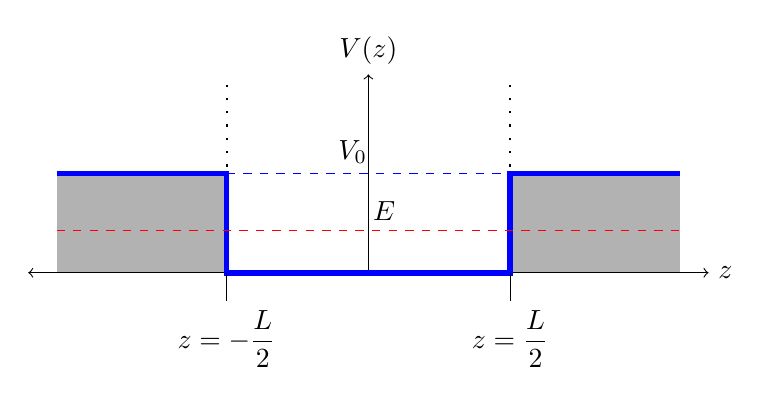
\begin{tikzpicture}[scale=1.8]

\fill[black!30] (-2.2,0) rectangle +(1.2,.7);
\fill[black!30] (1,0) rectangle +(1.2,.7);
\draw[<->](-2.4,0) -- (2.4,0)node[right]{$z$};
\draw[->](0,0) -- (0,1.4)node[above]{$V(z)$};

\draw[loosely dotted,thick] (-1,0) -- (-1,1.4);
\draw[loosely dotted,thick] (1,0) -- (1,1.4);

\draw[line width=2pt,blue](-2.2,.7) -- (-1,.7) -- (-1,0) -- (1,0) -- (1,.7) -- (2.2,.7);
\draw (-1,0) -- (-1,-.2) node[below,align=center,shift={(0,0)}] {$\displaystyle z=-\frac{L}{2}$};
\draw (1,0) -- (1,-.2) node[below,align=center,shift={(0,0)}] {$\displaystyle z=\frac{L}{2}$};

\draw[dashed,red](-2.2,.3) -- (2.2,.3) node[midway,above,black,shift={(.2,0)}]{$E$};

\draw[dashed,blue](-1,.7) -- (1,.7) node[midway,above,black,shift={(-.2,0)}]{$V_0$};

\end{tikzpicture}
\caption[][2cm]{ }
\label{fig:301}
\end{figure}
%

\sol We know what the energy eigenfunctions are. We need to find the lowest energy even solution, though. We plug in the parameters for an electron into Eq.~(\ref{eq:transprarams}) and get $\xi_0\approx 3.62$. We then numerically solve Eq.~(\ref{eq:transend}) to get $\xi_1 \approx 1.23$.\arnote{Check that you can do this using a computer. The integrals, too.} That means that our wave numbers are
\beq
k_1 \approx 0.246\;\rmt{nm}^{-1} \rmt{ and } \kappa_1 = \frac{2}{L}\sqrt{\xi_0^2 - \xi^2} \approx 0.69\;\rmt{nm}^{-1}.
\eeq
Now we know from Eq.~(\ref{eq:CArelation}) that \beq
C= A \E{\sqrt{\xi_0^2 - \xi^2}}\cos\xi \approx 10.7 A.
\eeq 
We now normalize $\psi_E^\rmt{(e)}(z)$:
\beq
1=\intii \abs{\psi_E^\rmt{(e)}(z)}^2 dz = \begin{cases} 0.084\abs{A}^2 & \rmt{Zone I}\\
6.28\abs{A}^2 & \rmt{Zone II}\\
0.084\abs{A}^2 & \rmt{Zone III}
\end{cases}.
\eeq
This means that $A\approx0.4$ and $C\approx4.3$. Our normalized energy eigenfunction for the first even-parity bound energy is thus
\beq
\psi_E^\rmt{(e)}(z) \approx \begin{cases} 4.3\E{(0.69\rmt{ nm}^{-1})z} & z \leq -5\rmt{ nm}\\
0.39 \cos((.246\rmt{ nm}^{-1}) z) & -5\rmt{ nm} \leq z \leq 5\rmt{ nm}\\
4.3\E{-(0.69\rmt{ nm}^{-1})z} & z \geq 5\rmt{ nm}
\end{cases}
\eeq
The energy of the electron is about 0.93~meV which is pretty far down the well.

\assess We checked the boundary conditions and the normalization and they all came pretty close, given our numerical approximations. The energy eigenfunction looks right (Fig.~\ref{fig:301b}), too with even parity and no wiggles.
\begin{marginfigure}
\centering
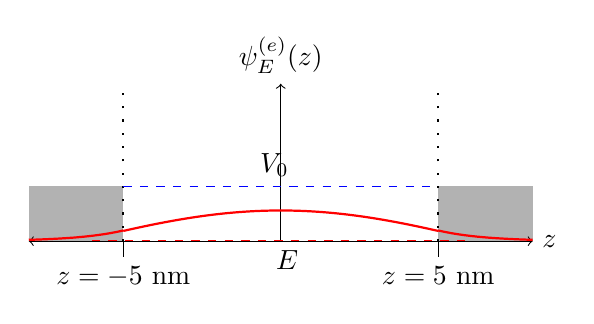
\begin{tikzpicture}[x=0.4cm,y=1cm]

\fill[black!30] (-8,0) rectangle +(3,.7);
\fill[black!30] (5,0) rectangle +(3,.7);
\draw[<->](-8,0) -- (8,0)node[right]{$z$};
\draw[->](0,0) -- (0,2)node[above]{$\psi_E^\rmt{(e)}(z)$};

\draw[loosely dotted,thick] (-5,0) -- (-5,2);
\draw[loosely dotted,thick] (5,0) -- (5,2);

\draw (-5,0) -- (-5,-.2) node[below,align=center,shift={(0,0)}] {$z=-5$~nm};
\draw (5,0) -- (5,-.2) node[below,align=center,shift={(0,0)}] {$z=5$~nm};

\draw[dashed,red](-6,.01) -- (6,.01) node[midway,below,black,shift={(.2,0)}]{$E$};

\draw[dashed,blue](-5,.7) -- (5,.7) node[midway,above,black,shift={(-.2,0)}]{$V_0$};

\draw[domain=-8:-5,samples=100,red,thick] plot({\x},{4.3*exp(0.69*\x)});
\draw[domain=5:8,samples=100,red,thick] plot({\x},{4.3*exp(-0.69*\x)});
\draw[domain=-5:5,samples=100,red,thick] plot({\x},{.39*cos(0.246*\x*180/3.14)});

\end{tikzpicture}
\caption{ }
\label{fig:301b}
\end{marginfigure}

\end{example}

\begin{exercise}
What are the eigenenergies and normalized eigenfunctions of the other even-parity states of  an electron in a 10~nm thick quantum well with an energy depth of 20~meV? Plot the eigenfunctions.
%\xi_0=3.62,\xi=3.45, k=0.690\rmt{ nm}^{-1} \kappa=0.219\rmt{ nm}^{-1}, C/A=-2.86, A=.323, C=-.924
\end{exercise}

\subsection{Odd-Parity Eigenfunctions}

We repeat the same procedure, starting with Eq.~(\ref{eq:bothparitysolution}), but this time working with the odd-parity wavefunction $\psi^\rmt{II,(o)} = B\sin kz$. The other change is that, since we are odd parity, $\psi_E(z) = -\psi_E(-z)$, so we get that $G = -C$.

\begin{exercise}
What is the condition to determine the allowed energies for odd-parity eigenfunctions (like Eq.~(\ref{eq:transend}) was for the even-parity eigenfunctions)?
%$\rmt{cot}\,\xi = -\sqrt{\frac{\xi_0^2}{\xi^2}-1}
\end{exercise}

\begin{exercise}
What is the lowest energy odd-parity eigenfunction for an electron in a 10~nm thick quantum well with an energy depth of 20~meV? Plot the eigenfunction. How does the energy compare to the even-parity energies?
%\xi_0=3.62,\xi=2.41, k=0.482\rmt{ nm}^{-1} \kappa=0.54\rmt{ nm}^{-1}, C/A=-9.95, A=.382, C=3.76
\end{exercise}

\section{Transitions}
Finally, we'd like to know the oscillator strengths for transitions between energy states. We know from Eq.~(\ref{eq:oscstr}) that 
\beq
f_{ab} = \frac{2}{3} \frac{m_e}{\hbar^2}\left|E_a - E_b\right|\abs{\bra{\psi_a}\hat{Z}\ket{\psi_b}}^2.
\eeq
We can simplify this using our wave number parameters:
\beq
f_{ab} = \frac{1}{3} \left|k^2_a - k^2_b\right|\abs{\bra{\psi_a}\hat{Z}\ket{\psi_b}}^2.
\eeq
So once we know the energies and eigenfunctions, we can calculate the oscillator strengths for those transitions. We'll model the transitions as being driven by $z$-polarized ElMaWs.

\begin{exercise}
What are the transition strengths between the different bound states for an electron in a 10~nm thick quantum well with an energy depth of 20~meV?
%1 even to 2 even: f_{1e2e}=0, 1 even to 1 odd: f_{1e1o}=0.626, 1 odd to 2 even: f_{1o2e}=0.325

\end{exercise}



%---------------------------------------
\chapter{Multiple Wells and Tunneling}


\begin{marginfigure}
\begin{tikzpicture}

%top
\begin{scope}[canvas is xz plane at y=1.5,shift={(0,0,0)}]
\fill[black!20] (-1,-1) rectangle +(2,2);
\end{scope}

%right
\begin{scope}[canvas is yz plane at x=1]
\fill[black!40] (-.2,-1) rectangle +(.4,2);

\fill[black!60] (.2,-1) rectangle +(.7,2);
\fill[black!50] (.9,-1) rectangle +(.6,2);
\fill[black!60] (-.9,-1) rectangle +(.7,2);
\fill[black!50] (-1.5,-1) rectangle +(.6,2);

\end{scope}

%front
\begin{scope}[canvas is xy plane at z=1,shift={(0,0,0)}]
\fill[black!30] (-1,-.2) rectangle +(2,.4);
\fill[black!40] (-1,.2) rectangle +(2,.7);
\fill[black!30] (-1,.9) rectangle +(2,.6);
\fill[black!30] (-1,-1.5) rectangle +(2,.6);
\fill[black!40] (-1,-.9) rectangle +(2,.7);
\end{scope}

\draw[dashed](0,0,0) -- (1,0,0);
\draw[->](1,0,0) -- (2,0,0)node[right]{$y$};
\draw[dashed](0,0,0) -- (0,1.5,0);
\draw[->](0,1.5,0) -- (0,2,0)node[right]{$z$};
\draw[dashed](0,0,0) -- (0,0,1);
\draw[->](0,0,1) -- (0,0,2)node[right]{$x$};

\draw[<->](-1.2,-.2,1)--(-1.2,.2,1) node[midway,left]{$a$};

\draw[<->](-1.8,-.9,1)--(-1.8,.9,1) node[midway,left]{$b$};

\node at (2,1.5,0){Material \#3};
\node at (2,-1.5,0){Material \#3};
\node at (2.3,0.4,0){Material \#1};

\node at (2.15,.9,0){Material \#2};
\node at (2.15,-.5,0){Material \#2};

\end{tikzpicture}
\end{marginfigure}
There are a number of situations where a quantum system such as an atom or an electron is confined to a well that is finite, but has neighboring wells. We saw with the finite quantum well model that some of the wavefunction extended into the classically forbidden space outside the well. What happens if there is another well nearby --- close enough that these wavefunction tails reach the second well? We'll now model that situation. Our picture is going to be a multiple layer quantum well for an electron. We'll model the middle Material \#1 as having a potential $V_0$ and the outer Material \#3 as being much higher in potential than anything else. Thus we'll model them as infinitely high. Finally, we model Material \#2 as our wells with $V=0$. As before, we'll focus on the $z$-direction and work in the position basis. The potential is sketched schematically in Figure~\ref{fig:doublewellfig}.
%
\begin{figure}
\centering
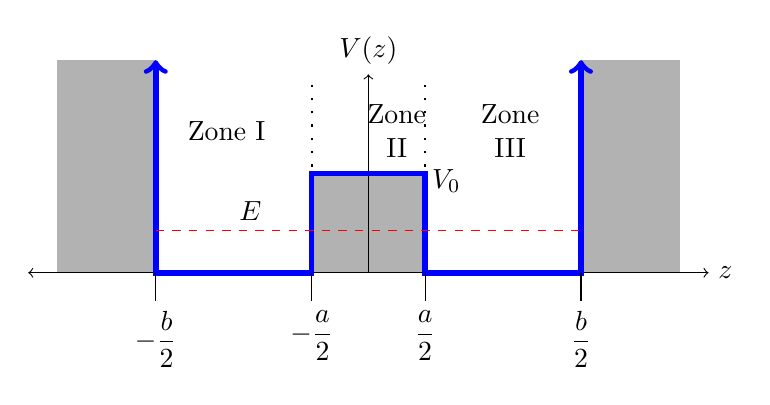
\begin{tikzpicture}[scale=1.8]

\fill[black!30] (-2.2,0) rectangle +(.7,1.5);
\fill[black!30] (1.5,0) rectangle +(.7,1.5);
\fill[black!30] (-.4,0) rectangle +(.8,.7);

\draw[<->](-2.4,0) -- (2.4,0)node[right]{$z$};
\draw[->](0,0) -- (0,1.4)node[above]{$V(z)$};

\draw[loosely dotted,thick] (-.4,0) -- (-.4,1.4);
\draw[loosely dotted,thick] (.4,0) -- (.4,1.4);

\draw[<->,line width=2pt,blue](-1.5,1.5) -- (-1.5,0) -- (-.4,0) -- (-.4,.7) -- (.4,.7) -- (.4,0) -- (1.5,0) -- (1.5,1.5);

\draw (-1.5,0) -- (-1.5,-.2) node[below,align=center,shift={(0,0)}] {$\displaystyle -\frac{b}{2}$};
\draw (1.5,0) -- (1.5,-.2) node[below,align=center,shift={(0,0)}] {$\displaystyle \frac{b}{2}$};

\draw (-.4,0) -- (-.4,-.2) node[below,align=center,shift={(0,0)}] {$\displaystyle -\frac{a}{2}$};
\draw (.4,0) -- (.4,-.2) node[below,align=center,shift={(0,0)}] {$\displaystyle \frac{a}{2}$};

\draw[dashed,red](-1.5,.3) -- (1.5,.3) node[midway,above,black,shift={(-1.5,0)}]{$E$};


\node[text width=1cm,align=center] at (.55,.65){$V_0$};

\node[text width=1cm,align=center] at (-1,1){Zone I};

\node[text width=1cm,align=center] at (.2,1){Zone II};
\node[text width=1cm,align=center] at (1,1){Zone III};

\end{tikzpicture}
\caption[][1cm]{Double well with inner barrier width $a$ and outer barrier total width $b$.}
\label{fig:doublewellfig}
\end{figure}
%
As before, we need to work in the three zones and determine the wavefunction in each zone, joining them together with our boundary conditions.

\section{Wavefunction Solutions}

Because $V=0$ in Zones I and III, we can use the same tools we used in the finite quantum well. The wavenumber is
\beq
k = \sqrt{\frac{2 m E}{\hbar^2}}
\eeq
and the solutions to the TISWE are the sum of sines and cosines. Except this time we will write them as the sum of two imaginary exponentials, since that will simplify our work later. We have, then, for Zones I and III
\bas
\psi^\rmt{I}(z) = & A\E{-\I k z} + B\E{\I k z}\\
\psi^\rmt{III}(z) = & F\E{-\I k z} + G\E{\I k z}.
\eas
Similarly, we follow the finite well model in Zone II. We have wavenumber 
\beq
\kappa = \sqrt{\frac{2 m}{\hbar^2}(V_0 - E)}
\eeq
and exponential solutions
\beq
\psi^\rmt{II}(z) = C\E{-\kappa z} + D\E{\kappa z} \rightarrow C\rmt{cosh}\;\kappa z + D\rmt{sinh}\;\kappa z
\eeq\marginnote[-1cm]{Note that cosh(z)$=1/2(\E{z} + \E{-z})$ and sinh(z)$=1/2(\E{z} - \E{-z})$.}%
which we re-write in terms of cosh and sinh in order to distinguish the even-parity and odd-parity solutions.

\subsection{Boundary Conditions}
Following Technique \ref{tactis:TISWEBC}, we now need to apply the boundary conditions (BCs) to determine the allowable energies. The wavefunction must go to zero at $\pm b/2$, must be continuous at $\pm a/2$ and must be smooth at $\pm a/2$.

Starting with the BCs at $\pm b/2$, we see that $\psi^\rmt{I}(-b/2)=0$. This means that\arnote[1cm]{Solve both of these and simplify.}%
\beq
\psi^\rmt{I}(z) = -2\I A \E{\I k b/2}\sin\left(kz + kb/2\right).
\eeq
Similarly we find
\beq
\psi^\rmt{III}(z) = -2\I F \E{-\I k b/2}\sin\left(kz - kb/2\right).
\eeq
However, we notice that the pieces in front of the sine terms are all just constants. So we can absorb these into the normalization constants $A$ and $F$. If we write the Zone I and III wavefunctions as
\bas
\psi^\rmt{I}(z) = & A \sin(kz + kb/2)\\
\psi^\rmt{III}(z) = & F\sin(kz - kb/2),
\eas
then we've matched the boundary conditions and we have the arbitrary normalization constant in front.

\section{Even-parity Wavefunctions}
As before, we now choose to work with the even-parity solutions first. \marginnote{The odd parity solutions will be an exercise.} That means we're looking at
\beq
\psi^\rmt{II}(z) =  C \rmt{cosh}\;\kappa z
\eeq
in Zone II. We now need to match the continuous and smooth BCs at $\pm a/2$. As before, we focus on one of the boundaries and divide the continuous and smooth BCs:\arnote[1cm]{Work all of this out in your notes.}
\beq
\begin{split}
\frac{\psi^\rmt{I}(-a/2) = \psi^\rmt{II}(-a/2)}{\left.\frac{d\psi^\rmt{I}}{dz}\right|_{-a/2} = \left.\frac{d\psi^\rmt{II}}{dz}\right|_{-a/2}}\rightarrow \\ \frac{1}{k}\tan\left(\frac{k}{2}(b-a)\right)=-\frac{1}{\kappa}\rmt{coth}\;\frac{\kappa a}{2}.
\end{split}
\label{eq:unsimpbcsmqw}
\eeq
In order to have energy eigenfunctions that match the boundary conditions, we need to find values for $E$ that satisfy this relationship. As before, we define the unitless parameters $\xi$ and $\xi_0$ using a form similar to Eq.~(\ref{eq:transprarams}) to make this a unitless problem:
\beq
\xi \equiv kb/2 =\sqrt{\frac{m b^2 E}{2\hbar^2}}  \rmt{ and } \xi_0 \equiv \sqrt{\frac{m b^2 V_0}{2\hbar^2}}.
\eeq
This makes our BCs from Eq.~(\ref{eq:unsimpbcsmqw}) to the unitless
\beq
\sqrt{\frac{\xi_0^2}{\xi^2}-1}\tan\left[\xi\left(1-\frac{a}{b}\right)\right] = -\rmt{coth}\;\left(\frac{a}{b}\sqrt{\xi_0^2 - \xi^2}\right).
\label{eq:simpbcsmqw}
\eeq

\begin{exercise}
Show that Eq.~(\ref{eq:unsimpbcsmqw}) becomes the unitless Eq.~(\ref{eq:simpbcsmqw}).
\end{exercise}

\begin{exercise}
Show that the equivalent condition for the odd-parity wavefunctions to Eq.~(\ref{eq:simpbcsmqw}) is
\beq
\sqrt{\frac{\xi_0^2}{\xi^2}-1}\tan\left[\xi\left(1-\frac{a}{b}\right)\right] = -\rmt{tanh}\;\left(\frac{a}{b}\sqrt{\xi_0^2 - \xi^2}\right)
\eeq
\end{exercise}

\begin{example}
\label{ex:nitrogen}
The nitrogen atom in the ammonia molecule can be in one of two possible wells on the right-hand or left-hand side of the hydrogen atoms. What are the lowest two bound-state energies for the nitrogen atom if the $0.2$~eV barrier has width  $a\approx20$~pm and the well width is $b\approx100$~pm?

\model We will model the ammonia molecule double well as a double square well with infinite walls on the outside. We'll model the nitrogen atom as a quantum system and use the tools we've built to find the bound-state energies.

\vis We have a situation that looks like Figure \ref{fig:nh3fig} where the nitrogen can be in either state.
\begin{figure}
\centering
\includegraphics[width=0.6\textwidth]{250px-Nitrogen-inversion-3D-balls.png}
\caption[][1cm]{ }
\label{fig:nh3fig}
\end{figure}

\sol We want the bound-state, even-parity energies. We'll solve Eq.~(\ref{eq:simpbcsmqw}) numerically. We get $\xi_0 \approx 18.3$ and $a/b \approx 0.2$. Solving the equation, we get $\xi_{1,e} \approx 3.674$ which gives an energy of $E_{1,e} \approx 8.06$~meV. We get the first odd-parity solution very close at $\xi_{1,o} \approx 3.675$ which gives an energy of $E_{1,o} \approx 8.07$~meV.\arnote[-1cm]{I skipped a lot of steps here. Make sure you can do these calculations.}

\assess The actual energy difference between the first two states is about 100~$\mu$eV, so our crude model isn't quite right. But it gives an idea of the possible bound states.

\end{example}

\section{Static and Dynamic Wavefunctions}

We now move forward and get an idea of what the energy eigenfunctions look like. We'll use the same model as in Example \ref{ex:nitrogen} in order to have concrete numbers to work with.

\begin{example}
\label{ex:ammoniaeigen}
What are the first even-parity and odd-parity wavefunctions for the nitrogen atom double-well model for ammonia?

\model Our model is the same as before. 

\vis Our potential well is the same as before. Explicitly, we have something that looks like Figure \ref{fig:ammoniafig}.
\begin{figure}
\centering
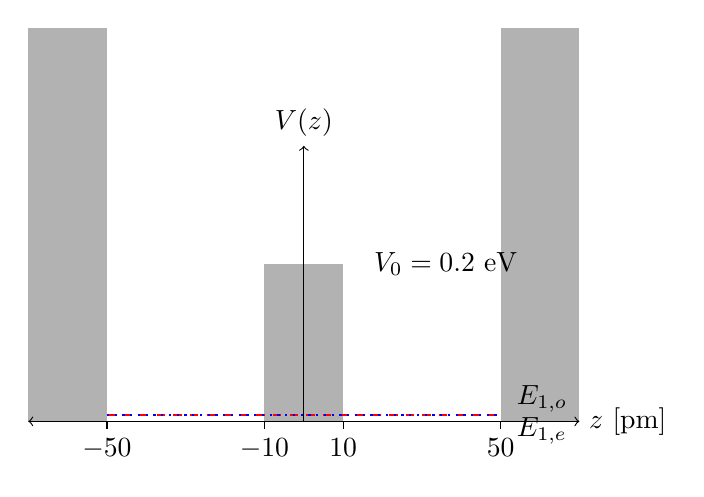
\begin{tikzpicture}[x=0.05cm,y=10cm]

\fill[black!30] (-70,0) rectangle +(20,.5);
\fill[black!30] (-10,0) rectangle +(20,0.2);
\fill[black!30] (50,0) rectangle +(20,.5);

\draw[<->](-70,0) -- (70,0)node[right]{$z$ [pm]};
\draw[->](0,0) -- (0,.35)node[above]{$V(z)$};


\draw (-50,0) -- (-50,-.01) node[below,align=center,shift={(0,0)}] {$-50$};
\draw (50,0) -- (50,-.01) node[below,align=center,shift={(0,0)}] {$50$};

\draw (-10,0) -- (-10,-.01) node[below,align=center,shift={(0,0)}] {$-10$};
\draw (10,0) -- (10,-.01) node[below,align=center,shift={(0,0)}] {$10$};


\draw[dashed,thick,red](-50,.008) -- (50,.008) node[right,black,shift={(1.5,-.02)}]{$E_{1,e}$};

\draw[dotted,thick,blue](-50,.0081) -- (50,.0081) node[right,black,shift={(1.5,0.02)}]{$E_{1,o}$};

\node[align=center] at (36,.2){$V_0 = 0.2$~eV};

\end{tikzpicture}
\caption[][1cm]{Double well with inner barrier width $20$~pm and outer barrier total width $100$~pm.}
\label{fig:ammoniafig}
\end{figure}

\sol We need to know the wave numbers and then we can normalize our energy eigenfunctions. We have
\bas
k_{1,e}\approx&0.07348\rmt{ pm}^{-1} & \kappa_{1,e} \approx&0.359\rmt{ pm}^{-1} \\
k_{1,o}\approx&0.0735\rmt{ pm}^{-1} & \kappa_{1,o} \approx&0.359\rmt{ pm}^{-1}.
\eas
We now find the even parity eigenfunction. 
\beq
\psi_E^\rmt{(e)}(z) = 
\begin{cases}
\psi^\rmt{I,(e)}(z) = A \sin\left(kz + kb/2\right),\\
& {}\\
\psi^\rmt{II,(e)}(z) = C \rmt{cosh}\; \kappa z\\
& {}\\
\psi^\rmt{III,(e)}(z) = F \sin\left(kz - kb/2\right).
\end{cases}
\eeq
The BC at $\pm a/2$ means that 
\beq
C =  A \frac{\sin\left[\frac{k}{2}(b-a)\right]}{\rmt{cosh}\; \kappa a/2}
\eeq
and the fact that the wavefunction is even parity means that $F = -A$. We now normalize this, using our known values for $k$, $\kappa$, $a$, and $b$. We get a normalization constant of $A \approx 0.153$ and an eigenfunction of
\beq
\psi_E^\rmt{(e)}(z) = 
\begin{cases}
 0.153 \sin\left(0.074 z + 3.67\right) & -50 \leq z \leq -10\\
& {}\\
0.0017 \rmt{cosh}\; (.359 z) & -10  \leq z \leq 10\\
& { }\\
 -  0.153 \sin\left(0.074 z - 3.67\right) & {10  \leq z \leq 50 }.
\end{cases}
\eeq
\begin{marginfigure}[-3cm]
\begin{sagesilent}
x=var('x')
t = var('t')
x_coords = [t for t in srange(-10,10,.1)]
y_coords = [0.5*0.0017*(exp(-0.3585*t)+exp(0.3585*t)) for t in srange(-10,10,.1)]
output34 = ""
for i in range(0,len(x_coords)-1):
    output34 += r"\draw[red, thick] (%f ,%f )--(%f  ,%f );"%(x_coords[i],y_coords[i],x_coords[i+1],y_coords[i+1])
\end{sagesilent}

\centering
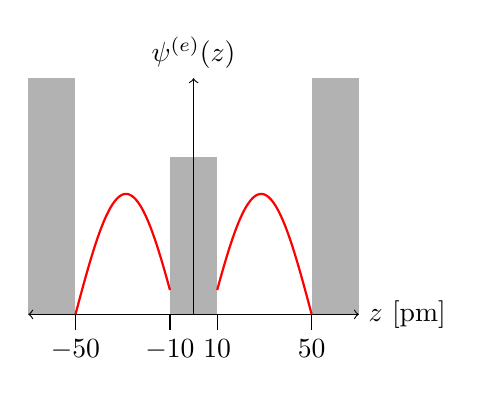
\begin{tikzpicture}[x=0.03cm,y=10cm]

\fill[black!30] (-70,0) rectangle +(20,.3);
\fill[black!30] (-10,0) rectangle +(20,.2);
\fill[black!30] (50,0) rectangle +(20,.3);

\draw[<->](-70,0) -- (70,0)node[right]{$z$ [pm]};
\draw[->](0,0) -- (0,.3)node[above]{$\psi^\rmt{(e)}(z)$};


\draw (-50,0) -- (-50,-.02) node[below,align=center,shift={(0,0)}] {$-50$};
\draw (50,0) -- (50,-.02) node[below,align=center,shift={(0,0)}] {$50$};

\draw (-10,0) -- (-10,-.02) node[below,align=center,shift={(0,0)}] {$-10$};
\draw (10,0) -- (10,-.02) node[below,align=center,shift={(0,0)}] {$10$};

\draw[domain=-50:-10,samples=100,red,thick] plot({\x},{.153*sin((0.0734*\x+3.67)*180/3.14)});
\sagestr{output34}
\draw[domain=10:50,samples=100,red,thick] plot({\x},{.153*sin((-0.0734*\x+3.67)*180/3.14)});

\end{tikzpicture}
\caption{ }
\label{fig:ex312a}
\end{marginfigure}
where $z$ is measured in picometers. This wavefunction is shown in Fig.~\ref{fig:ex312a}. We repeat the process for the first odd-parity eigenfunction to get
\beq
\psi_E^\rmt{(o)}(z) = 
\begin{cases}
 0.153 \sin\left(0.074 z + 3.67\right) & -50 \leq z \leq -10\\
& {}\\
-0.0017 \rmt{sinh}\; (0.359 z) & -10  \leq z \leq 10\\
& { }\\
  0.153 \sin\left(0.074z - 3.67\right) & {10  \leq z \leq 50 }.
\end{cases}
\eeq
This wavefunction is shown in Figure \ref{fig:ex312b}.
\begin{marginfigure}
\begin{sagesilent}
x=var('x')
t = var('t')
x_coords = [t for t in srange(-10,10,.1)]
y_coords = [0.5*0.0017*(exp(-0.3585*t)-exp(0.3585*t)) for t in srange(-10,10,.1)]
output35 = ""
for i in range(0,len(x_coords)-1):
    output35 += r"\draw[blue, thick] (%f ,%f )--(%f  ,%f );"%(x_coords[i],y_coords[i],x_coords[i+1],y_coords[i+1])
\end{sagesilent}

\centering
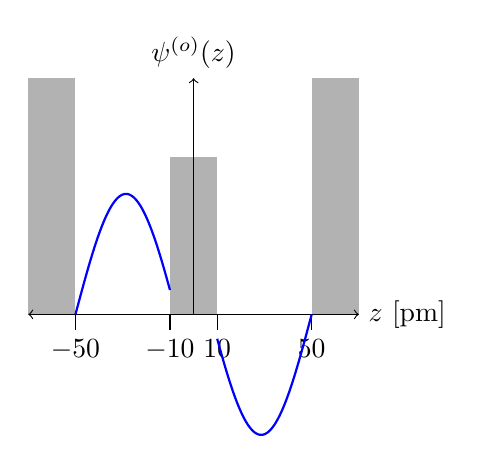
\begin{tikzpicture}[x=0.03cm,y=10cm]

\fill[black!30] (-70,0) rectangle +(20,.3);
\fill[black!30] (-10,0) rectangle +(20,.2);
\fill[black!30] (50,0) rectangle +(20,.3);

\draw[<->](-70,0) -- (70,0)node[right]{$z$ [pm]};
\draw[->](0,0) -- (0,.3)node[above]{$\psi^\rmt{(o)}(z)$};


\draw (-50,0) -- (-50,-.02) node[below,align=center,shift={(0,0)}] {$-50$};
\draw (50,0) -- (50,-.02) node[below,align=center,shift={(0,0)}] {$50$};

\draw (-10,0) -- (-10,-.02) node[below,align=center,shift={(0,0)}] {$-10$};
\draw (10,0) -- (10,-.02) node[below,align=center,shift={(0,0)}] {$10$};

\draw[domain=-50:-10,samples=100,blue,thick] plot({\x},{.153*sin((0.0734*\x+3.67)*180/3.14)});
\sagestr{output35}
\draw[domain=10:50,samples=100,blue,thick] plot({\x},{-.153*sin((-0.0734*\x+3.67)*180/3.14)});

\end{tikzpicture}
\caption{ }
\label{fig:ex312b}
\end{marginfigure}

\assess Both eigenfunctions integrate to one, so they are normalized. They are the right shape, continuous, and smooth.

\end{example}

\begin{exercise}
Show the work needed to get the even and odd energy eigenfunctions in Example \ref{ex:ammoniaeigen}.
\end{exercise}

\section{Tunneling}
The energy eigenfunctions we found in the last section are all stationary states. The quantum system stays in a state where it is found in both wells with equal probability. However, we are interested in the situation where the state starts in one well. We now apply that initial condition and look at the evolution of the wavefunction. 

We will model the same situation as before - a nitrogen atom in the double-well potential potential of an ammonia molecule. We will model this as the double square well as before. We want the system to start in a single well, so we'll model the initial state as an equal superposition of the even and odd eigenstates,
\beq
\Psi(z,0) = \frac{1}{\stwo}\left(\psi_{E}^\rmt{(e)}(z) + \psi_{E}^\rmt{(o)}(z) \right).
\eeq
This wavefunction is visualized in Figure \ref{fig:twostatesuper31}.

\begin{marginfigure}
\begin{sagesilent}
x=var('x')
t = var('t')
x_coords = [t for t in srange(-10,10,.1)]
y_coords = [0.707*(0.5*0.0017*(exp(-0.3585*t)-exp(0.3585*t)) + 0.5*0.0017*(exp(-0.3585*t)+exp(0.3585*t))) for t in srange(-10,10,.1)]
output36 = ""
for i in range(0,len(x_coords)-1):
    output36 += r"\draw[purple, thick] (%f ,%f )--(%f  ,%f );"%(x_coords[i],y_coords[i],x_coords[i+1],y_coords[i+1])
\end{sagesilent}

\centering
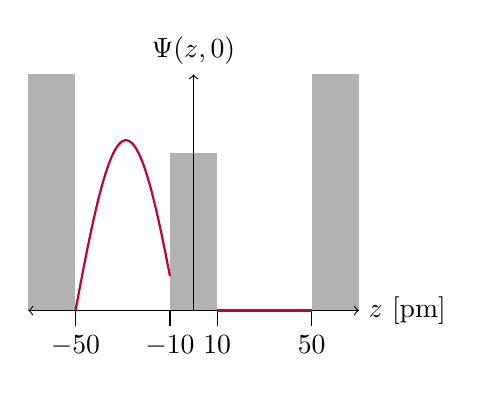
\begin{tikzpicture}[x=0.03cm,y=10cm]

\fill[black!30] (-70,0) rectangle +(20,.3);
\fill[black!30] (-10,0) rectangle +(20,.2);
\fill[black!30] (50,0) rectangle +(20,.3);

\draw[<->](-70,0) -- (70,0)node[right]{$z$ [pm]};
\draw[->](0,0) -- (0,.3)node[above]{$\Psi(z,0)$};


\draw (-50,0) -- (-50,-.02) node[below,align=center,shift={(0,0)}] {$-50$};
\draw (50,0) -- (50,-.02) node[below,align=center,shift={(0,0)}] {$50$};

\draw (-10,0) -- (-10,-.02) node[below,align=center,shift={(0,0)}] {$-10$};
\draw (10,0) -- (10,-.02) node[below,align=center,shift={(0,0)}] {$10$};

\draw[domain=-50:-10,samples=100,purple,thick] plot({\x},{0.707*(.153*sin((0.0734*\x+3.67)*180/3.14) + .153*sin((0.0734*\x+3.67)*180/3.14))});
\sagestr{output36}
\draw[domain=10:50,samples=100,purple,thick] plot({\x},{0.707*(-.153*sin((-0.0734*\x+3.67)*180/3.14) +.153*sin((-0.0734*\x+3.67)*180/3.14) )});


\end{tikzpicture}
\caption{ }
\label{fig:twostatesuper31}
\end{marginfigure}
The time evolution of the state is then
\beq
\Psi(z,t) = \frac{1}{\stwo}\left(\psi_{E}^\rmt{(e)}(z) \E{-\I E_\rmt{(e)} t/\hbar} + \psi_{E}^\rmt{(o)}(z)\E{-\I E_\rmt{(o)} t/\hbar} \right).
\eeq
The probability of measuring the system in its initial state is thus\arnote[1cm]{Work out the trig identity in the last step.}%
\bas
P(\Psi(z,0)) =& \abs{\avg{\Psi(z,0)|\Psi(z,t)}}^2= \abs{ \intii \Psi^*(z,0)\Psi(z,t) dz }^2\\
=& \abs{\frac{1}{2}\left(\E{-\I E_\rmt{(e)} t/\hbar} + \E{-\I E_\rmt{(o)} t/\hbar}\right)}^2 \\
= & \cos^2\left(\frac{\Delta\omega t}{2}\right)
\eas
where $\Delta\omega = ( E_\rmt{(o)} -  E_\rmt{(e)})/\hbar$. So the probability of measuring the state in the initial well drops to zero after a time $t = \pi/\Delta\omega$. It then returns to its initial configuration with a period of $T_\rmt{tunnel} = 2\pi/\Delta\omega$. We can write this in terms of the dimensionless well parameters $\xi_\rmt{(e)}$ and $\xi_\rmt{(o)}$:
\beq
T_\rmt{tunnel} = \frac{\pi m b^2}{\hbar}\frac{1}{\xi_\rmt{(o)}^2 - \xi_\rmt{(e)}^2}.
\eeq
The deeper the potential well, the smaller the difference between the two dimensionless parameters will be, and the longer the tunneling period.

\begin{example}
What is the tunneling period for the nitrogen atom we've been modeling?

\model Our model is the same as before. We now model the initial configuration of the nitrogen atom as being on one side of the molecule.

\vis The same picture applies.

\sol The energy difference between the even- and odd-parity states is $\Delta E \approx 0.01$~meV. That means that the frequency difference is $\Delta\omega \approx 15.1\times10^{9}$~rad/s. That gives a tunneling period of about 0.4~ns. That time scale is about right for molecular dynamics.

\end{example}

\begin{exercise}
An electron is confined to a double quantum well structure where the barrier is $5$~nm wide and has a potential of $0.5$~eV. The wells on either side are each $20$~nm wide and the next material has a very high potential barrier. If the electron is injected into one of the two wells, what is the approximate tunneling time?
%11 hours!
\end{exercise}



%---------------------------------------
\chapter{Quantum Harmonic Oscillator: Position Basis}

\section{Harmonic Potentials}

\begin{marginfigure}[2cm]
\centering
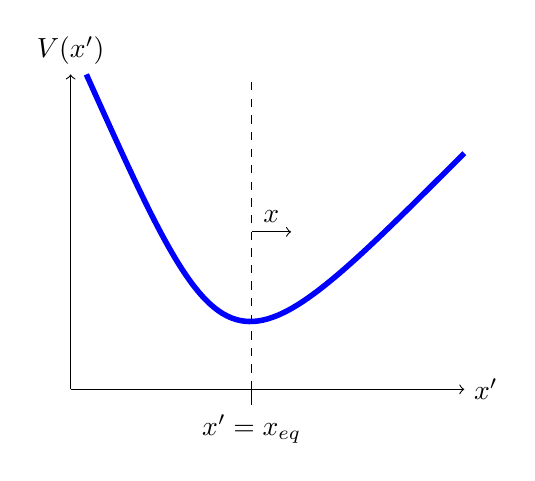
\begin{tikzpicture}
\draw[->] (0,0) -- (5,0)node[right]{$x'$};
\draw[->] (0,0) -- (0,4)node[above]{$V(x')$};
\draw[line width=2pt,blue](0.2,4) ..controls(2,0) .. (5,3) ;
\draw(2.3,0) -- (2.3,-.2)node[below]{$x' = x_\rmt{eq}$};
\draw[dashed](2.3,0) -- (2.3,4);
\draw[->](2.3,2) -- (2.8,2)node[midway,above]{$x$};
\end{tikzpicture}
\end{marginfigure}
There are a number of situations where a quantum object is in some kind of bound state with a potential that varies smoothly in some dimension. If the potential has a local minimum at $x' = x_\rmt{eq}$, we can approximate the potential with a quadratic series expansion about that equilibrum point. We'll define the coordinate $x\equiv x' - x_\rmt{eq}$ so that 
\bas
V(x') =& V(x_\rmt{eq} + x) \approx V(x_\rmt{eq}) + x \left.\frac{dV}{dx'}\right|_{x'=x_\rmt{eq}} + \frac{1}{2} \left(\left.\frac{d^2V}{dx'^2}\right|_{x'=x_\rmt{eq}}\right) x^2 \\
\approx & V(x_\rmt{eq}) + \frac{1}{2} k x^2
\eas
because $dV/dx' = 0$ at an equilibrium position and we've defined 
\beq
k\equiv \left.\frac{d^2V}{dx'^2}\right|_{x'=x_\rmt{eq}},
\eeq
which is positive at the local minimum at $x' = x_\rmt{eq}$. The total mechanical energy, and thus the Hamiltonian, for a system in one-dimension in this type of simple harmonic oscillator (SHO) potential is
\beq
H_\rmt{SHO} = \frac{p_x^2}{2m} + \frac{1}{2}k x^2,
\eeq
where $p_x$ and $m$ are the momentum and mass of the system, respectively. There is a natural frequency scale for the SHO: $\omega_0 \equiv \sqrt{k/m}$. We insert this into the Hamiltonian to get
\beq
H_\rmt{SHO} = \frac{p_x^2}{2m} + \frac{1}{2}m \omega_0^2 x^2.
\eeq

\section{SHO in the Position Basis}
\label{sec:shoposition}
We now follow our general techniques for modeling the quantum system in a SHO. We convert the Hamiltonian to an operator:
\beq
\hat{H} = \frac{1}{2m}\hat{P}_x^2 + \frac{1}{2}m \omega_0^2\hat{X}^2.
\label{eq:onedqhoop}
\eeq
We now need to decide what basis to work with. There are both momentum and position operators in this Hamiltonian, so we could potentially work in either basis. Because the potential is written in terms of a position basis operator, we'll work in the position basis. We then convert the Schr\"{o}dinger equation to the TISWE, since our potential is time-independent. That gives us\marginnote{\ref{tool:TISWE}}%
\beq
-\frac{\hbar^2}{2m}\frac{d^2\psi_E(x)}{dx^2} + \frac{1}{2}m\omega_0^2 x^2 \psi_E(x) = E\psi_E(x).
\label{eq:shotiswe}
\eeq
We now need to solve this second-order differential equation. We look up the solutions in a math table\marginnote{I actually use my \CAS for this kind of thing - it keeps the constants straight for me.} and find that the solutions are in terms of {\em Parabolic Cylinder D} functions, denoted $D_\nu(\xi)$. The solutions to Eq.~(\ref{eq:shotiswe}) are
\beq
\psi_E(x) = A\;D_{\left(\frac{E}{\hbar \omega_0} - \frac{1}{2}\right)}\left(\I\sqrt{\frac{2m\omega_0}{\hbar}}x\right) + B\; D_{\left(\frac{E}{\hbar \omega_0} - \frac{1}{2}\right)}\left(\sqrt{\frac{2m\omega_0}{\hbar}}x\right).
\eeq
We now apply the BCs to determine the constants $A$ and $B$ and to determine the conditions, if any, on the total energy $E$. The first condition is that $D_\nu(\I\xi)$ does not converge at $\pm\infty$. That means we must set the coefficient $A=0$. Furthermore, we find that $D_\nu(\xi)$ only converges at $\pm\infty$ if $\nu$ is a positive or zero integer. That means we have the condition
\beq
\frac{E}{\hbar \omega_0} - \frac{1}{2} = n \rmt{ where } n = 0,1,2,3,\ldots.
\eeq
Rewriting this, we see that the energy $E_n$ comes in quantized steps
\beq
E_n = \left(n + \frac{1}{2}\right)\hbar\omega_0.
\eeq
Finally, we normalize the energy eigenfunctions so that\arnote{Check the integral on your own. Again, I recommend using a \CAS here.}
\beq
1 = \intii \psi_E^*(x)\psi_E(x) dx = \abs{B}^2(n!)\sqrt{2\pi}\sqrt{\frac{\hbar}{2m\omega_0}}.
\eeq
Finally, we note that there is a natural length scale here\marginnote{Some people define this without the $\sqrt{2}$ in the denominator. I like it better this way.}
\beq
\Delta x_0\equiv \sqrt{\frac{\hbar}{2m\omega_0}}
\label{eq:qholengthscale}
\eeq
which we can use in the argument of the Parabolic Cylinder D functions. We put this all together to get the energy eigenfunctions, which are now denoted $\psi_n(x) \equiv \avg{x|E_n}$ to indicate that they depend on the integer $n$:
\beq
\psi_n(x) = \frac{1}{\left(2\pi\right)^{1/4}}  \frac{1}{\sqrt{ n! \Delta x_0}}D_n\left(\frac{x}{\Delta x_0}\right).
\eeq
\marginnote{
The first four states are:
\bas
\psi_0(x) = & \frac{\E{-x^2/(4\Delta x_0^2)}}{(2\pi)^{1/4}\sqrt{\Delta x_0}}\\
\psi_1(x) = & \frac{\E{-x^2/(4\Delta x_0^2)}}{(2\pi)^{1/4}\sqrt{\Delta x_0}}\;\frac{x}{\Delta x_0}\\
\psi_2(x) = & \frac{\E{-x^2/(4\Delta x_0^2)}}{(2\pi)^{1/4}\sqrt{\Delta x_0}}\;\left(\frac{x^2}{\sqrt{2}\Delta x_0^2} - \frac{1}{\sqrt{2}}\right)\\
\psi_3(x) = & \frac{\E{-x^2/(4\Delta x_0^2)}}{(2\pi)^{1/4}\sqrt{\Delta x_0}}\;\left(\frac{x^3}{\sqrt{6}\Delta x_0^3} - \frac{3x}{\sqrt{6}\Delta x_0}\right)
\eas
}%
Because $n$ is an integer, this also can be written in terms of the Hermite polynomials
\beq
\psi_n(x) = \frac{1}{\left(2\pi\right)^{1/4}} \frac{\E{-x^2/(4\Delta x_0^2)}}{\sqrt{ 2^n n!\Delta x_0}}H_n\left(\frac{x}{\sqrt{2}\Delta x_0}\right).
\eeq
The first four energy eigenfunctions are graphed in Figure \ref{eq:SHOeigen}. As we've seen before, there are even-parity and odd-parity eigenfunctions. We also see that as the energy increases (with increasing $n$), the number of zero-crossings in the wavefunction also increases. 
\begin{figure}
\centering
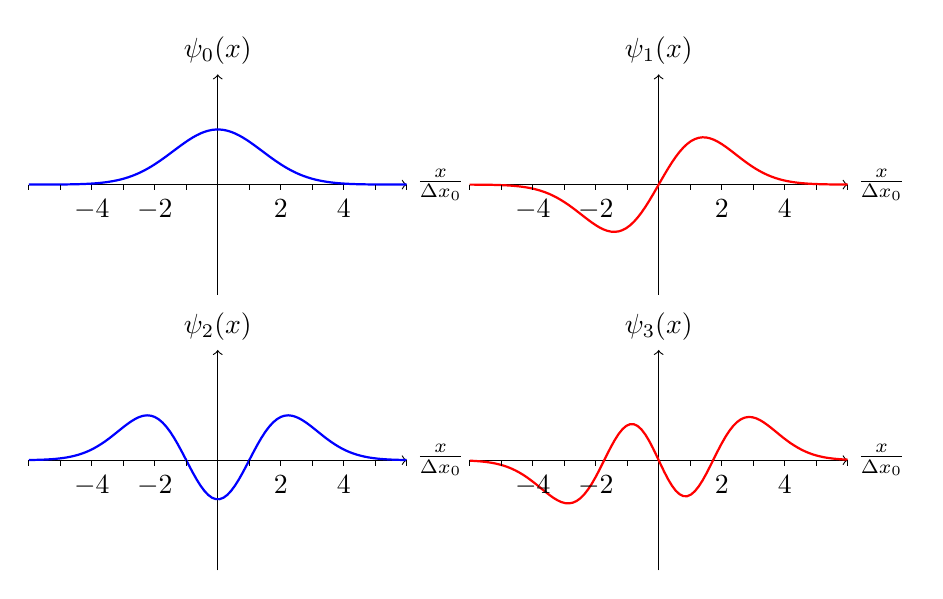
\begin{tikzpicture}[x=0.4cm,y=.7cm]
\begin{scope}[shift={(-7,0)}]
\draw[->](-6,0) -- (6,0)node[right]{$\frac{x}{\Delta x_0}$};
\draw[->](0,-2) -- (0,2)node[above]{$\psi_0(x)$};
\draw[domain=-6:6,samples=100,blue,thick] plot({\x},{exp(-((\x)^2)/4)});
\foreach \t in {-4,-2,2,4}{
\draw(\t,0) -- (\t,-.1) node[below]{$\t$};
}
\foreach \t in {-6,-5,-3,-1,1,3,5,6}{
\draw(\t,0) -- (\t,-.1);
}
\end{scope}
\begin{scope}[shift={(7,0)}]
\draw[->](-6,0) -- (6,0)node[right]{$\frac{x}{\Delta x_0}$};
\draw[->](0,-2) -- (0,2)node[above]{$\psi_1(x)$};
\draw[domain=-6:6,samples=100,red,thick] plot({\x},{exp(-((\x)^2)/4)*\x});
\foreach \t in {-4,-2,2,4}{
\draw(\t,0) -- (\t,-.1) node[below]{$\t$};
}
\foreach \t in {-6,-5,-3,-1,1,3,5,6}{
\draw(\t,0) -- (\t,-.1);
}
\end{scope}
\begin{scope}[shift={(-7,-5)}]
\draw[->](-6,0) -- (6,0)node[right]{$\frac{x}{\Delta x_0}$};
\draw[->](0,-2) -- (0,2)node[above]{$\psi_2(x)$};
\draw[domain=-6:6,samples=100,blue,thick] plot({\x},{exp(-((\x)^2)/4)*(0.71*(\x)^2-0.71)});
\foreach \t in {-4,-2,2,4}{
\draw(\t,0) -- (\t,-.1) node[below]{$\t$};
}
\foreach \t in {-6,-5,-3,-1,1,3,5,6}{
\draw(\t,0) -- (\t,-.1);
}
\end{scope}
\begin{scope}[shift={(7,-5)}]
\draw[->](-6,0) -- (6,0)node[right]{$\frac{x}{\Delta x_0}$};
\draw[->](0,-2) -- (0,2)node[above]{$\psi_3(x)$};
\draw[domain=-6:6,samples=100,red,thick] plot({\x},{exp(-((\x)^2)/4)*(((\x)^3)/2.45- \x*1.22)});
\foreach \t in {-4,-2,2,4}{
\draw(\t,0) -- (\t,-.1) node[below]{$\t$};
}
\foreach \t in {-6,-5,-3,-1,1,3,5,6}{
\draw(\t,0) -- (\t,-.1);
}
\end{scope}
\end{tikzpicture}
\caption[][2cm]{The first four energy eigenfunctions.}
\label{eq:SHOeigen}
\end{figure}

\begin{exercise}
Show that, for the quantum SHO, the average position measurement of the ground state $\psi_0(x)$ is
\beq
\avg{\hat{X}} = 0,
\eeq
and that the average
\beq
\avg{\hat{X}^2} = \Delta x_0^2.
\eeq

\end{exercise}

\begin{example}
\label{ex:trappedca}
A single calcium ion is trapped in a harmonic Paul trap with trap frequency $\omega_0 = (2\pi) 2.5$~MHz and is cooled to the ground state $\psi_0(x)$. What is the uncertainty if we measure the ion's position?

\model We model the calcium ion (mass 40 amu) as a quantum system in a quantized SHO. Since the atom is in the ground state, we can use the results from above to calculate its measurement uncertainty since
\beq
\Delta X = \sqrt{\avg{\hat{X}^2} - \avg{\hat{X}}^2}.
\eeq

\vis We are modeling the atom as being in the ground state wavefunction $\psi_0(x)$ as shown in Figure \ref{eq:SHOeigen}.

\sol We know that $\avg{\hat{X}}=0$ and that $\avg{\hat{X}^2}=\Delta x_0^2$. This means that the uncertainty in the measurement is just the constant $\Delta x_0$:
\beq
\Delta x_0 = \sqrt{\frac{\hbar}{2 m \omega_0}} \approx 7.1\rmt{ nm}.
\eeq

\assess The spread in the wavefunction is larger than we would expect for the size of an atom (about 0.1~nm), but it seems like it is on the right scale.

\end{example}

\section{Dynamics and Transitions in the QSHO}
\label{sec:qshodynamics}
As we've seen before, once we have the eigenfunctions for the Hamiltonian, we can write the time-dependent wavefunction for an arbitrary state
\beq
\psi(x,t) = \sum_n a_n \E{-\I E_n t/\hbar} \psi_n(x).
\eeq

We now model transistions between energy eigenstates in the quantum SHO. The energies are
\beq
E_n = \left(n + \frac{1}{2}\right)\hbar\omega_0 \rmt{ where } n = 0,1,2,3,\ldots.
\eeq
The first thing to note is that there is a lowest energy state where $n=0$. We can make transitions down to this energy state, but not below it. We plot the first four probability densities at vertical spacings of $\Delta E = \hbar \omega_0$ in Figure \ref{fig:qshoenergy}. We convert the spring constant to energy units using the definition for $k$, $E_0$ and $\Delta x_0$ so that
\beq
k = \frac{E_0}{\Delta x_0^2}.
\eeq%
\begin{figure}
\centering
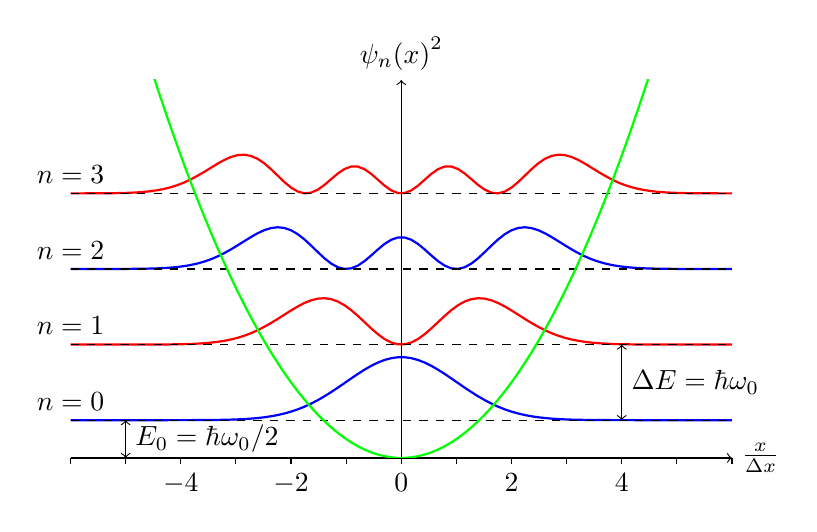
\begin{tikzpicture}[x=0.7cm,y=.8cm]

\draw[->](-6,0) -- (6,0)node[right]{$\frac{x}{\Delta x}$};
\draw[->](0,0) -- (0,6)node[above]{$\abs{\psi_n(x)}^2$};
\begin{scope}[shift={(0,0.6)}]
\draw[domain=-6:6,samples=100,blue,thick] plot({\x},{(exp(-((\x)^2)/4))^2});
\draw[dashed](-6,0)node[above]{$n=0$}--(6,0);
\end{scope}

\begin{scope}[shift={(0,1.8)}]
\draw[domain=-6:6,samples=100,red,thick] plot({\x},{(exp(-((\x)^2)/4)*\x)^2});
\draw[dashed](-6,0)node[above]{$n=1$}--(6,0);
\end{scope}

\begin{scope}[shift={(0,3.0)}]
\draw[domain=-6:6,samples=100,blue,thick] plot({\x},{(exp(-((\x)^2)/4)*(0.71*(\x)^2-0.71))^2});
\draw[dashed](-6,0)node[above]{$n=2$}--(6,0);
\end{scope}

\begin{scope}[shift={(0,4.2)}]
\draw[domain=-6:6,samples=100,red,thick] plot({\x},{(exp(-((\x)^2)/4)*(((\x)^3)/2.45- \x*1.22))^2});
\draw[dashed](-6,0)node[above]{$n=3$}--(6,0);
\end{scope}

\begin{scope}
\clip (-6,0) rectangle + (12,6);
\draw[domain=-6:6,samples=100,green,thick] plot({\x},{0.3*(\x)^2});
\end{scope}

\draw[<->] (4,0.6) -- (4,1.8) node[midway,right]{$\Delta E = \hbar \omega_0$};

\draw[<->] (-5,0) -- (-5,0.6) node[midway,right]{$E_0 = \hbar \omega_0/2$};

\foreach \t in {-4,-2,0,2,4}{
\draw(\t,0) -- (\t,-.1) node[below]{$\t$};
}
\foreach \t in {-6,-5,-3,-1,1,3,5,6}{
\draw(\t,0) -- (\t,-.1);
}

\end{tikzpicture}
\caption[][2cm]{The first four energy probability densities.}
\label{fig:qshoenergy}
\end{figure}%
%
We also note that there are definite parity states. Because of this, the expectation values
\beq
\avg{\hat{X}} = \avg{E_n|\hat{X}|E_n} = \intii \psi_n^*(x) x \psi_n(x) dx = 0.
\eeq
This is because $x$ is odd-parity and, since $\psi_n$ is real, $\abs{\psi_n(x)}^2$ is even parity. The product of those two, integrated over an even interval, is zero.

\begin{exercise}
Use an analogous argument using the parity of the wavefunctions to show that
\beq
\avg{\hat{P}_x} = 0.
\eeq
\end{exercise}

\begin{exercise}
What is the uncertainty relationship for the ground state energy eigenfunction:
\beq
\Delta X \Delta P_x?
\eeq
\end{exercise}

If we model transitions as being driven by ElMaWs polarized in the $x$-direction, then the oscillator strength\marginnote{Recall that the oscillator strength gives a relative probability for the transition to happen.} from Eq.~(\ref{eq:oscstr}) for a transition between two energy eigenstates is
\beq
f_{nm} = \frac{2}{3} \frac{m}{\hbar^2}\left|E_n - E_m\right|\abs{\bra{\psi_n}\hat{X}\ket{\psi_m}}^2.
\eeq
The matrix elements have the same form as the expectation value for the position. We therefore make the same argument - the only way the oscillator strength will be non-zero if if we make the transition from an odd-parity state to an even-parity state or vice-versa.

\begin{example}
What is the oscillator strength for the transition of a trapped calcium ion (as in Example \ref{ex:trappedca}) between the ground state and the first excited state?

\model We are modeling this as we did before- the calcium ion is in the ground state and we are coupling and ElMaW with energy $\hbar \omega_0$ on resonance.

\vis The transition is between the ground state and the first excited state- we need the overlap integral between these two. The solid curve is $\psi_0$, the dashed is $\psi_1$ and the dotted curve is $\psi_0 x\psi_1$. We've graphed this in Figure \ref{fig:ex322}.

\begin{figure}
\centering
\begin{tikzpicture}[x=0.7cm,y=1cm]
\draw[->](-6,0) -- (6,0)node[right]{$\frac{x}{\Delta x}$};
\draw[->](0,-2) -- (0,2)node[above]{$\psi(x)$};
\draw[domain=-6:6,samples=100,blue,thick] plot({\x},{exp(-((\x)^2)/4)});
\draw[domain=-6:6,samples=100,red,thick,dashed] plot({\x},{exp(-((\x)^2)/4)*\x});
\draw[domain=-6:6,samples=100,purple,thick,dotted] plot({\x},{(exp(-((\x)^2)/4)*\x)^2});
\foreach \t in {-4,-2,2,4}{
\draw(\t,0) -- (\t,-.1) node[below]{$\t$};
}
\foreach \t in {-6,-5,-3,-1,1,3,5,6}{
\draw(\t,0) -- (\t,-.1);
}

\end{tikzpicture}
\caption[][2cm]{ }
\label{fig:ex322}
\end{figure}

\sol The overlap integral is
\beq
\abs{\bra{\psi_1}\hat{X}\ket{\psi_0}}^2 = \abs{\intii \psi_1(x)x\psi_0(x)dx}^2 = \Delta x_0^2.
\eeq
So the oscillator strength is (where $E_{n+1} - E_n = \hbar\omega_0$)
\beq
f_{10} = \frac{2}{3} \frac{m}{\hbar^2}\left(\hbar\omega_0\right)\Delta x_0^2 = \frac{1}{3}.
\eeq

\assess The oscillator strength is unitless and in the right range.

\end{example}

\begin{exercise}

Make a table of the oscillator strengths for a transition between any two of the first $10$ energy eigenstates of the quantum SHO.

\end{exercise}



%---------------------------------------
\chapter{Quantum Harmonic Oscillator: Number Basis}
\label{ch:numberbasis}
There is another way to model the quantum simple harmonic oscillator. This technique involves working some operator algebra, but it will eventually get us to the same solution. One of the reasons to do this is that we will build a new model for working with operators that will be useful again later. We start by modeling our one-dimensional quantum simple harmonic oscillator with the Hamiltonian operator from Eq.~(\ref{eq:onedqhoop}):
\beq
\hat{H} = \frac{1}{2m}\hat{P}_x^2 + \frac{1}{2}m \omega_0^2\hat{X}^2.
\eeq
This operators is the sum of two squares and can be factorized like this\marginnote{Mathematically $d^2 + e^2 = (d+ \I e)(d - \I e)$.}%
\beq
\left(\sqrt{\frac{m \omega_0^2}{2}}\hat{X}+\frac{\hat{P}_x }{\I\sqrt{2m}} \right)\left(\sqrt{\frac{m \omega_0^2}{2}}\hat{X}-  \frac{\hat{P}_x }{\I\sqrt{2m}}\right).
\eeq
However, there is a problem with this. Because $\com{\hat{X},\hat{P}_x}= \I\hbar$, the expansion of this product isn't quite right; we actually get\arnote{Do this expansion in your notes.}% 
\beq
\I \frac{\omega_0}{2}\left(\com{\hat{X},\hat{P}_x}\right) = -\frac{\hbar\omega_0}{2}.
\eeq
So the Hamiltonian is actually 
\bas
\hat{H} = &\left(\sqrt{\frac{m \omega_0^2}{2}}\hat{X}+\frac{\hat{P}_x }{\I\sqrt{2m}} \right)\left(\sqrt{\frac{m \omega_0^2}{2}}\hat{X}-  \frac{\hat{P}_x }{\I\sqrt{2m}}\right) + \frac{\hbar\omega_0}{2}\\
=& \left[\left(\sqrt{\frac{m \omega_0}{2\hbar}}\hat{X}+ \frac{\hat{P}_x }{\I\sqrt{2m\hbar\omega_0}}\right)\left(\sqrt{\frac{m \omega_0}{2\hbar}}\hat{X}- \frac{\hat{P}_x }{\I\sqrt{2m\hbar\omega_0}}\right) + \frac{1}{2}\right]\hbar\omega_0.
\eas
We define two new operators that are the quantities in the product\marginnote{Other quantum texts use the notation $\hat{a}^\dagger$ for this operator. That notation is confusing since it uses a lower-case letter and doesn't describe what it does. We will not use it.}
\beq
\begin{split}
\Ap \equiv & \left(\sqrt{\frac{m \omega_0}{2\hbar}}\hat{X}+ \frac{\hat{P}_x }{\I\sqrt{2m\hbar\omega_0}}\right)\\
\Am \equiv & \left(\sqrt{\frac{m \omega_0}{2\hbar}}\hat{X}- \frac{\hat{P}_x }{\I\sqrt{2m\hbar\omega_0}}\right).
\end{split}
\label{eq:aplusaminus}
\eeq
Note that the two operators are related by the Hermitian conjugate $\Am^\dagger = \Ap$. The Hamiltonian is then
\beq
\hat{H} = \left(\Ap\Am + \frac{1}{2}\right)\hbar\omega_0.
\eeq
It now makes sense to work in a different basis than the position basis. We need to explore the properties of these new operators first to find their eigenvectors and eigenvalues. Once we have those, we will work in that basis to solve the time-independent Schr\"{o}dinger equation.

\section{Properties of $\Ap$ and $\Am$}
\label{sec:numberoperator}
The first thing to do is explore the commutation relationships. The first one is an exercise:

\begin{exercise}
Use the definition of the $\Ap$ and $\Am$ operators from Eq.~(\ref{eq:aplusaminus}) to show that
\beq
\com{\Am,\Ap} = 1
\eeq
\end{exercise}
Because the combination of the two operators $\Ap\Am$ appears in the Hamiltonian, we define a new operator that is the product of those two:
\beq
\hat{N} \equiv \Ap\Am.
\eeq
The commutation relationships between $\Apm$ and $\hat{N}$ tell us whether these operators commute with the Hamiltonian and are therefore a good starting point for finding an eigenvector basis. However, we find that
\bas
\com{\Ap,\hat{N}} =& \Ap\Ap\Am - \Ap\Am\Ap \\
=& \Ap\left(\Ap\Am - \Am\Ap\right) = -\Ap \rmt{ and }\\
\com{\Am,\hat{N}} =& \Am.
\eas
So these are not a good operator set to work with. However, we can work with the combination opeartor $\hat{N}$ since $\com{\hat{N},\hat{H}}=0$. We will call the eigenvectors of $\hat{N}$ $\ket{n}$ for now and then explore the meaning of this notation later on. So we start with
\beq
\hat{N}\ket{n} = n\ket{n}.
\eeq
We now look at what happens if we apply the operator $\hat{N}\left(\Ap\ket{n}\right)$:\arnote{Work out this first step on your own.}%
\bas
\hat{N}\left(\Ap\ket{n}\right) = & \Ap\left(\hat{N} + 1\right)\ket{n}\\
=&\Ap(n+1)\ket{n}\\
=&(n + 1)\left(\Ap\ket{n}\right).
\eas
That means that $\Ap\ket{n}$ is an eigenvector of $\hat{N}$ with eigenvalue $(n+1)$. That must mean that $\Ap\ket{n} = C_{+}\ket{n+1}$ where $C_{+}$ is a normalization constant. We now identify the operator $\Ap$ as a {\em raising operator} because when it acts on the eigenvector $\ket{n}$, it raises the number by one. 

\begin{exercise}
Show that the {\em lowering operator} $\Am$ acts similarly on the state $\ket{n}$:
\beq
\Am\ket{n} = C_{-} \ket{n-1}
\eeq
where $C_{-}$ is a normalization constant.

\end{exercise}

We now need to determine the normalization constants. We do this with the condition that our eigenvectors are normalized: $\avg{n|n} =1 $. That means that\arnote{Follow down each side of this argument.}%
\bas
\bra{n}\left(\Ap\right)^\dagger\left(\Ap\right)\ket{n} = & \bra{n}\Am\Ap\ket{n}\\
\downarrow\qquad &\quad \downarrow \nonumber\\
\abs{C_{+}}^2 =& n+1
\eas
which means that $C_{+} = \sqrt{n+1}$. Similarly, $C_{-} = \sqrt{n}$.\arnote{Work this one out, too.} Finally, we check the average of the $\hat{N}$ in the $\ket{n}$ basis:
\beq
\bra{n}\hat{N}\ket{n} = n\avg{n|n} = n. 
\eeq
But we also have that
\beq
\bra{n}\hat{N}\ket{n} = \left(\bra{n} \Am^\dagger\right) \Am\ket{n} = \avg{\Psi|\Psi}\geq 0
\eeq
which implies that $n\geq0$. So there is a minimum value to the eigenvectors and eigenvalues of the $\hat{N}$ operator, $\ket{n_\rmt{min}} = \ket{0}$ with eigenvalue $n_\rmt{min} = 0$. So if we repeatedly act with the lowering operator on an arbitrary eigenvector $\ket{n}$, we eventually reach this minimum state:
\beq
\Am\ket{n}\propto \ket{n-1};\; \Am\ket{n-1}\propto\ket{n-2}\;\ldots\; \Am\ket{n_\rmt{min}} = 0\ket{0}.
\eeq
This also means that
\beq
\hat{N}\ket{n_\rmt{min}} = \Ap\Am\ket{n_\rmt{min}} = \Ap\left(0\ket{0}\right) = 0\Ap\ket{0} = 0.
\eeq
We can also go the other way, staring with the $\ket{0}$ state and building to any arbitrary $\ket{n}$ state with the raising operator
\beq
\ket{n} = \frac{1}{\sqrt{n!}}\left(\Ap\right)^n\ket{0}.
\eeq
We now interpret this model: the operator $\hat{N}$ is the {\em number operator} whose eigenvectors $\ket{n}$ are a number basis with eigenvalues $n$. The number basis is a set of integer values $n\geq 0$ and is an orthonormal basis where\arnote{Use the raising and lowering operators to show this.}%
\beq
\avg{n|m} = \delta_{nm}.
\eeq
The raising and lowering operators move between the eigenvectors of the number basis with a minium eigenvector $\ket{n_\rmt{min}} = \ket{0}$ with eigenvalue $0$. Putting this all together, we have
\beq
\begin{split}
\Ap = & \left(\sqrt{\frac{m \omega_0}{2\hbar}}\hat{X}+ \frac{\hat{P}_x }{\I\sqrt{2m\hbar\omega_0}}\right)\\
\Am = & \left(\sqrt{\frac{m \omega_0}{2\hbar}}\hat{X}- \frac{\hat{P}_x }{\I\sqrt{2m\hbar\omega_0}}\right)\\
\Ap\ket{n} = & \sqrt{n+1}\ket{n+1}\\
\Am\ket{n} = & \sqrt{n}\ket{n-1}\\
\hat{N}\ket{n} = &\Ap\Am\ket{n} = n\ket{n},\; n=0,1,2,\ldots.
\end{split}
\eeq


\section{TISWE in the Number Basis}

We return to the Hamiltonian, written using the number operator
\beq
\hat{H} = \left(\hat{N} + \frac{1}{2}\right)\hbar\omega_0.
\eeq
The Hamiltonian acts on the number states
\bas
\hat{H}\ket{n} =& \left(\hat{N} + \frac{1}{2}\right)\hbar\omega_0\ket{n}\\
=&\left(n + \frac{1}{2}\right)\hbar\omega_0\ket{n}
\eas
so we see that the number states $\ket{n}$ are energy eigenvectors of the Hamiltonian with eigenvalues
\beq
E_n = (n + \frac{1}{2})\hbar\omega_0.
\eeq
We've seen these eigenvalues before--- they are the same eigenvalues associated with the energy eigenfunctions $\psi_n(x)$. That means that we can change between the two different bases by projecting the position basis on the number states\marginnote{\ref{tool:wavefunction}}%
\beq
\psi_n(x) = \avg{x|n}.
\eeq
Our model also lets us formulate the eigenfunctions by starting with the number basis states. Because $\bra{x}\Am\ket{0}=0$, we expand the lowering operator using Eq.~(\ref{eq:aplusaminus}) to get
\bas
0 =& \bra{x}\left(\sqrt{\frac{m \omega_0}{2\hbar}}\hat{X}- \frac{\hat{P}_x }{\I\sqrt{2m\hbar\omega_0}}\right)\ket{0}\\
=&\sqrt{\frac{m \omega_0}{2\hbar}}\bra{x}\hat{X}\ket{0}- \frac{1}{\I\sqrt{2m\hbar\omega_0}}\bra{x}\hat{P}_x \ket{0}
\eas
We insert $\onehat = \int\ket{x'}\bra{x'}dx'$ \marginnote{\ref{tool:span}} twice between the operators and the $\ket{0}$. We then use the definitions for the eigenfunctions in the position basis and the definitions of the matrix elements to get\arnote{Work out the steps in your notes.}%
\beq
\frac{d\psi_0(x)}{dx} = -\frac{m\omega_0}{\hbar}x\psi_0(x).
\eeq
This differential equation has (normalized) solution
\beq
\psi_0(x) = \left(\frac{m\omega_0}{\pi\hbar}\right)^{1/4}\E{-\frac{m\omega_0x^2}{2\hbar}}
\eeq
which is equivalent to what we found in Section \ref{sec:shoposition}. We can continue to operate on the number basis vectors to build up the other eigenfunctions.

\begin{example}
What is $\avg{\hat{X}}$ using the number basis?

\model We will model our system using the number basis.

\vis The number basis vectors, converted to the position basis, look just like we saw in Section \ref{sec:shoposition}.

\sol In the number basis, we have
\beq
\avg{\hat{X}} = \bra{n}\hat{X}\ket{n}.
\eeq
We need to rewrite Eq.~(\ref{eq:aplusaminus}) in order to find $\hat{X}$ in terms of $\Apm$. It is a bit of algebra\arnote[1.5cm]{Do this one in your notes, too!} to get
\beq
\begin{split}
\hat{X} = & \sqrt{\frac{\hbar}{2m\omega_0}}\left(\Am + \Ap\right)\\
\hat{P}_x = & -\I\sqrt{\frac{m\hbar\omega_0}{2}}\left(\Am - \Ap\right).
\end{split}
\label{eq:xhatphat}
\eeq\marginnote[-1cm]{The units for $\hat{X}$ are [length] and for $\hat{P}_x$ are [mass$\cdot$length/time] which are momentum units. That makes sense because in this basis $\ket{n}$ are unitless as are the eigenvalues $n$.}%
Therefore we have
\bas
\bra{n}\hat{X}\ket{n} =& \bra{n}\sqrt{\frac{\hbar}{2m\omega_0}}\left(\Am + \Ap\right)\ket{n}\\
=&\sqrt{\frac{\hbar}{2m\omega_0}}\bra{n}\left(\sqrt{n}\ket{n-1} + \sqrt{n+1}\ket{n+1}\right)\\
=0
\eas
because the number states are orthonormal.

\assess The result agrees with what we found previously for the quantum SHO.

\end{example}


\begin{exercise}
For a simple harmonic oscillator in the state $|n\rangle$, calculate
the following (using the raising and lowering operators---{\em no integrals!}):%
\bas
\rmt{(a) } \langle \hat{P}_{x}\rangle & &
\rmt{(b) }  \langle \hat{X}^{2}\rangle & &
\rmt{(c) } \langle \hat{P}_{x}^{2}\rangle\nonumber\\
\rmt{(d) } \Delta X & &
\rmt{(e) }  \Delta P_{x} & &
\rmt{(f) } \Delta X \Delta P_{x}\nonumber
\eas
Is the uncertainty principle satisfied?

\end{exercise}

\section{Transitions in the Number Basis}

We saw in Section \ref{sec:qshodynamics} that an ElMaW can drive transitions between neighboring eigenstates of the Hamiltonian. We now identify the raising and lowering operators in our model with dipole transitions between states. We also saw that the dipole transitions only couple nearest neighbors: $n$ to $n\pm1$. This agrees with our number state model where the raising and lowering operators only shift the number states by one.


\begin{exercise}
\label{ex:coherentstate}
The quantum mechanical state of a simple harmonic oscillator that most closely behaves like a classical state is a {\em coherent state}.   Furthermore, the quantum state of the ElMaW from an ideal laser is a coherent state of the electromagnetic field.  [Note: the Gaussian wave packet of a massive particle is also often called a coherent state.] Since they are so important, let's investigate how they relate to the simple harmonic oscillator.  \marginnote{For more discussion of these states, see S. Howard and S. K. Roy, {\em Am. J. Phys.} {\bf 55}, 1109 (1987).}

A coherent state for the simple harmonic oscillator $\ket{\alpha}$ is defined to be an eigenstate of the lowering operator $\Am$:
%
\begin{equation}
\Am\ket{\alpha} = \alpha\ket{\alpha},
\label{coherent eigen}
\end{equation}
%
where $\alpha$ is the eigenvalue.  Since $\Am$ is not Hermitian ($\Am^\dagger \neq \Am$), the eigenvalues $\alpha$ are generally complex: $\alpha^{*} \neq \alpha$, so the Hermitian congugate of Eq.~(\ref{coherent eigen}) must be written in terms of the raising operator $\Am^{\dag}$: 
%
\begin{equation}
\langle\alpha|\Am^{\dagger}=  \langle\alpha|\alpha^{*}.
\label{adjoint coherent eigen}
\end{equation}
%

\begin{enumerate}

\item[(a)]  Use these results and the methods used in the previous problem to show for a quantum simple harmonic oscillator in a coherent state ($|\psi\rangle = |\alpha\rangle$), 
%
\begin{equation}
\Delta X\Delta P_{x} = \frac{\hbar}{2},
\end{equation}
%
i.e., this state is the best one can hope for by the Heisenberg Uncertainty Principle.

\item[(b)]   The position wave function of a SHO coherent state can be written as
%
\begin{equation}
\Psi_{\alpha}(x,0) = \psi_{\alpha}(x) = \langle x|\alpha\rangle = \left(\frac{1}{2\pi\beta^{2}}\right)^{1/4}
              \E{-(x -x_{0})^{2}/4\beta^{2}},
\end{equation}
%
where $\beta$ is a constant having dimensions of length.  Does this lead to a  Gaussian position probability distribution?  If so, what is $\sigma$?

\item[(c)] Since this is not an eigenstate of the Hamiltonian, it will evolve with time with position probability density
%
\begin{equation}
|\Psi_{\alpha}(x,t)|^{2} = \frac{1}{\beta\sqrt{2\pi}}
            \E{-(x - x_{0}\cos\omega_{0} t)^{2}/2\beta^{2}}.
\end{equation}
%
 Use a \CAS to create an animation of $|\Psi(x,t)|^{2}$ using $\beta =
0.5$ \AA, $x_{0} = 1$ \AA, and $\omega_{0} = 1$~rad/s.  Does the system behave like a classical simple harmonic oscillator?  How does its behavior differ (besides the fact that it oscillates back and forth) from the Gaussian wave packet of the free-particle that you investigated earlier?

\end{enumerate}

\end{exercise}

%-------------------------------------------

\chapter{Part \ref{part3} Review and Test}
We started this part using the Matter Wave Model to model the interference of atoms or other quantum systems. We implemented a Gaussian wave packet model the create normalizable states that model the behavior of freely propagating systems. We then moved to bound systems and developed a model for describing the stationary states and dynamics of bound quantum systems. We applied this model to infinite quantum wells, finite quantum wells, multiple quantum wells, and the quantum harmonic oscillator. We also modeled transitions between two bound states and found that they will undergo Rabi oscillations.

It is important to practice using these tools to model experiments. The following set of exercises is a good way to test your understanding of these models. Try to do these without referring to the previous text. If you can do all of them and your solutions agree with those provided on the following pages, then you are in pretty good shape to move forward with the material. If not, you should specifically review the material  you do not have mastery of yet, then retry the test exercises.

\begin{exercise}
In a simple model of the Colella-Overhauser-Werner (COW) experiment, a Mach-Zehnder interferometer is rotated from a horizontal plane to a vertical plane such that the horizontal path CD is a height $H_{0}$ above the horizontal AB path:

{\centering\includegraphics[height=2in]{COW}}

A beam of neutrons each with momentum $p_{0}$ is incident upon beam splitter A which then splits the beam into upward and horizontal beams as shown.  One can show that in this configuration, the neutrons have a propagation amplitude $e^{i\alpha}$ for traveling the vertical paths AC or BD, where $\alpha$ depends on $p_{0}$, the gravitational acceleration $g$, and $H_{0}$.  Using energy conservation, one finds that the neutron's momentum traveling along the top horizontal path CD is $p_{CD} \simeq p_{0} - (m^{2}gH_{0})/p_{0}$, where $m$ is the mass of the neutron.


\begin{enumerate}
\item Find $\lambda_{CD}/\lambda_{0}$,  the ratio of the wavelength of the neutrons when they're traveling the top horizontal path CD compared to their incident wavelength $\lambda_{0}$.   Which is larger?

\item Find the probability that neutron will reach detector \#1.  
\end{enumerate}

\end{exercise}

\begin{exercise}
A quantum system with mass $m$ is trapped in a 1-D harmonic oscillator with characteristic frequency $\omega_0$. The system begins in a superposition state of the first two energy eigenstates:
\beq
\ket{\Psi(t=0)} = \frac{1}{2}\ket{0} + \frac{\I\sqrt{3}}{2}\ket{1}.
\eeq
What is the average momentum measurement as a function of time?
\end{exercise}

\begin{exercise}
A quantum system is trapped in a very deep 1-D potential that has a very small bump in the center of the well as shown in Figure ~\ref{fig:343}. What are the energies of the bound states in this system?

\begin{figure}
\centering
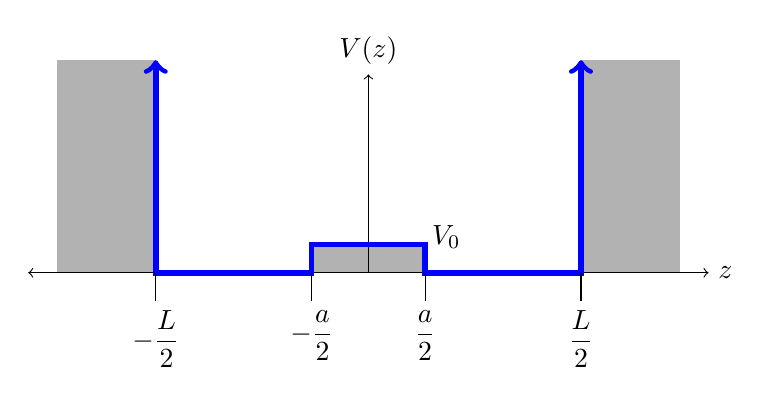
\begin{tikzpicture}[scale=1.8]

\fill[black!30] (-2.2,0) rectangle +(.7,1.5);
\fill[black!30] (1.5,0) rectangle +(.7,1.5);
\fill[black!30] (-.4,0) rectangle +(.8,.2);

\draw[<->](-2.4,0) -- (2.4,0)node[right]{$z$};
\draw[->](0,0) -- (0,1.4)node[above]{$V(z)$};

\draw[<->,line width=2pt,blue](-1.5,1.5) -- (-1.5,0) -- (-.4,0) -- (-.4,.2) -- (.4,.2) -- (.4,0) -- (1.5,0) -- (1.5,1.5);

\draw (-1.5,0) -- (-1.5,-.2) node[below,align=center,shift={(0,0)}] {$\displaystyle -\frac{L}{2}$};
\draw (1.5,0) -- (1.5,-.2) node[below,align=center,shift={(0,0)}] {$\displaystyle \frac{L}{2}$};

\draw (-.4,0) -- (-.4,-.2) node[below,align=center,shift={(0,0)}] {$\displaystyle -\frac{a}{2}$};
\draw (.4,0) -- (.4,-.2) node[below,align=center,shift={(0,0)}] {$\displaystyle \frac{a}{2}$};

\node[text width=1cm,align=center] at (.55,.25){$V_0$};

\end{tikzpicture}
\caption[][1cm]{Very deep well with a small bump in the middle}
\label{fig:343}
\end{figure}
\end{exercise}

\begin{exercise}
What are the bound state energies for a very narrow, very deep one-dimensional potential well, $V(x) = -\alpha \delta(x)$?

\end{exercise}

Stop here and don't continue reading until you have completed the exercises.
\newpage
\begin{example}
In a simple model of the Colella-Overhauser-Werner (COW) experiment, a Mach-Zehnder interferometer is rotated from a horizontal plane to a vertical plane such that the horizontal path CD is a height $H_{0}$ above the horizontal AB path:

{\centering\includegraphics[height=2in]{COW}}

A beam of neutrons each with momentum $p_{0}$ is incident upon beam splitter A which then splits the beam into upward and horizontal beams as shown.  One can show that in this configuration, the neutrons have a propagation amplitude $e^{i\alpha}$ for traveling the vertical paths AC or BD, where $\alpha$ depends on $p_{0}$, the gravitational acceleration $g$, and $H_{0}$.  Using energy conservation, one finds that the neutron's momentum traveling along the top horizontal path CD is $p_{CD} \simeq p_{0} - (m^{2}gH_{0})/p_{0}$, where $m$ is the mass of the neutron.
\begin{enumerate}
\item Find $\lambda_{CD}/\lambda_{0}$,  the ratio of the wavelength of the neutrons when they're traveling the top horizontal path CD compared to their incident wavelength $\lambda_{0}$.   Which is larger?
\item Find the probability that neutron will reach detector \#1.  
\end{enumerate}

\model We will model the neutrons as a quantum system with uniform incoming momentum. Because we are treating different paths, we will use the path-integral formalism and determine the overall phase of each path at the detector.

\vis The picture is shown above.

\sol 
\begin{enumerate}
\item We first look at the relative wavelengths of the initial state and the state moving across the top arm. Initially, we have a momentum of $p_0$, so the corresponding wavelength is $\lambda = h/p_0$ or, similarly, $k_0 = p_0/\hbar$. The wavelength across the top is then
\beq
\lambda_{CD} = h/p_{CD} = \frac{h}{p_0 - (m^{2}gH_{0})/p_{0}}.
\eeq
Therefore, the ratio of the two wavelengths is
\beq
\frac{\lambda_{CD}}{\lambda_0}= \frac{p_0}{p_{CD}} = \frac{1}{1-\frac{m^2 g H_0}{p_0^2}} >1.
\eeq
So we have $\lambda_{CD}>\lambda_0$.
\item In order to find the probability of detection at detector \#1, we need the total phase of each path. We start with path $\Psi_{ABD}$:
\bas
\Psi_{ABD} =& \psi_{BS,A}^{T}\psi_{A\rightarrow B}\psi_{MB}\psi_{B\rightarrow D}\psi_{BS,D}^{R}\\
= &\frac{1}{\stwo}\E{\I k_0 L_0}(-1)\E{\I\alpha}\frac{\I}{\stwo}.
\eas
The other path is then
\bas
\Psi_{ACD} =& \psi_{BS,A}^{R}\psi_{A\rightarrow C}\psi_{MB}\psi_{C\rightarrow D}\psi_{BS,D}^{T}\\
= &\frac{\I}{\stwo}\E{\I\alpha}(-1)\E{\I k_{CD} L_0}\frac{1}{\stwo}.
\eas
We insert in the wavenumber for the top path and then find the magnitude squared:
\bas
\Pd =& \abs{\Psi}^2 = \abs{\psi_{ABD} + \psi_{ACD}}^2\\
=& \frac{1}{4}\abs{1+ \E{\I m^2 g H_0 L_0/(\hbar p_0)}}^2\\
=& \frac{1}{2}\left(1+ \cos\frac{m^2 g H_0 L_0}{\hbar p_0} \right)
\eas
\end{enumerate}

\assess The units check out correctly on the cosine phase. This looks similar to our other modified interferometers in that the phase difference between the two arms, due to the different gravitational potential, leads to a change in the probability of detecting at detector \#1.


\end{example}

\begin{example}
A quantum system with mass $m$ is trapped in a 1-D harmonic oscillator with characteristic frequency $\omega_0$. The system begins in a superposition state of the first two energy eigenstates:
\beq
\ket{\Psi(t=0)} = \frac{1}{2}\ket{0} + \frac{\I\sqrt{3}}{2}\ket{1}.
\eeq
What is the average momentum measurement as a function of time?

\model We model this as a one-dimensional quantum harmonic oscillator (QHO). We know that the energies are $E_n = (n+1/2)\hbar\omega_0$ for the QHO.

\vis We are starting in a superposition state, so our wavefunction will begin looking something like the sum shown in Fig~\ref{fig:342a}.
\begin{figure}
\centering
\begin{tikzpicture}[x=0.7cm,y=1cm]
\draw[->](-6,0) -- (6,0)node[right]{$\frac{x}{\Delta x}$};
\draw[->](0,-2) -- (0,2)node[above]{$\psi(x)$};
\draw[domain=-6:6,samples=100,blue,thick] plot({\x},{1/2*exp(-((\x)^2)/4)});
\draw[domain=-6:6,samples=100,red,thick,dashed] plot({\x},{sqrt(3)/2*exp(-((\x)^2)/4)*\x});
\draw[domain=-6:6,samples=100,purple,thick,dotted] plot({\x},{1/2*exp(-((\x)^2)/4) + sqrt(3)/2*exp(-((\x)^2)/4)*\x});
\foreach \t in {-4,-2,2,4}{
\draw(\t,0) -- (\t,-.1) node[below]{$\t$};
}
\foreach \t in {-6,-5,-3,-1,1,3,5,6}{
\draw(\t,0) -- (\t,-.1);
}

\end{tikzpicture}
\caption[][2cm]{ }
\label{fig:342a}
\end{figure}

\sol We first find the time evolution of the quantum state using what we know if the energies for the first two eigenstates:
\beq
\ket{\Psi(t)} = \frac{1}{2}\E{\I \omega_0 t/2}\ket{0} + \frac{\I\sqrt{3}}{2}\E{3\I \omega_0 t/2}\ket{1}.
\eeq
We now find the average angular momentum measurement for this quantum state:
\bas
\bra{\Psi}\hat{P}_x\ket{\Psi} = & \bra{\Psi}\left(-\I\sqrt{\frac{m \hbar \omega_0}{2}}\left[\Am - \Ap \right] \right)\ket{\Psi} \\
=&\sqrt{\frac{3 m \hbar \omega_0}{8}}\cos \omega_0 t,
\eas
where we've used the properties of the raising and lowering operators and the orthogonality of the number states to simplify the average.

\assess The units are correct: we get kg$\cdot$m/s for the units. We find that the average momentum starts at a maxima, then oscillates between zero and the maximum momentum. That makes sense, given that the state is in a harmonic oscillator.

\end{example}

\begin{example}
A quantum system is trapped in a very deep 1-D potential that has a very small bump in the center of the well as shown in Figure ~\ref{fig:344}. What are the energies of the bound states in this system?

\model We are going to model this as a small perturbation to the infinite quantum well. Because we are only interested in the energies of the system, we'll use what we know if the eigenfunctions of the infinite quantum well to find the energy shift due to the perturbation.

\vis

\begin{figure}
\centering
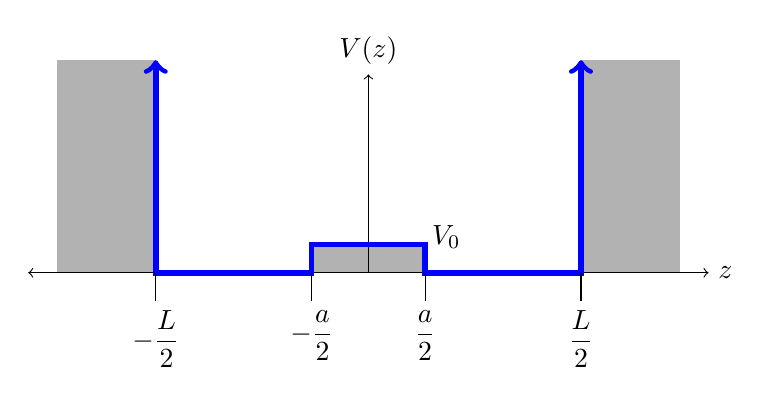
\begin{tikzpicture}[scale=1.8]

\fill[black!30] (-2.2,0) rectangle +(.7,1.5);
\fill[black!30] (1.5,0) rectangle +(.7,1.5);
\fill[black!30] (-.4,0) rectangle +(.8,.2);

\draw[<->](-2.4,0) -- (2.4,0)node[right]{$z$};
\draw[->](0,0) -- (0,1.4)node[above]{$V(z)$};

\draw[<->,line width=2pt,blue](-1.5,1.5) -- (-1.5,0) -- (-.4,0) -- (-.4,.2) -- (.4,.2) -- (.4,0) -- (1.5,0) -- (1.5,1.5);

\draw (-1.5,0) -- (-1.5,-.2) node[below,align=center,shift={(0,0)}] {$\displaystyle -\frac{L}{2}$};
\draw (1.5,0) -- (1.5,-.2) node[below,align=center,shift={(0,0)}] {$\displaystyle \frac{L}{2}$};

\draw (-.4,0) -- (-.4,-.2) node[below,align=center,shift={(0,0)}] {$\displaystyle -\frac{a}{2}$};
\draw (.4,0) -- (.4,-.2) node[below,align=center,shift={(0,0)}] {$\displaystyle \frac{a}{2}$};

\node[text width=1cm,align=center] at (.55,.25){$V_0$};

\end{tikzpicture}
\caption[][1cm]{Very deep well with a small bump in the middle}
\label{fig:344}
\end{figure}

\sol We know that the eigenfunctions of the unperturbed infinite quantum well are given in Eq.~(\ref{eq:psiforinfwell}):

\beq
\psi_{Z,n}(z) = \begin{cases}
\displaystyle \sqrt{\frac{2}{L}} \cos\left(\frac{n\pi z}{L}\right) &\displaystyle \abs{z}\leq\frac{L}{2},\; n = 1,3,5,\ldots\\
&\\
\displaystyle \sqrt{\frac{2}{L}} \sin\left(\frac{n\pi z}{L}\right) &\displaystyle \abs{z}\leq\frac{L}{2},\; n = 2,4,6,\ldots\\
& \\
0 & \displaystyle\abs{z}>\frac{L}{2},
\end{cases}
\eeq
where we've calculated the normalization constant for both the even and odd eigenfunctions. The energy shift due to the perturbation was determined in Eq.~(\ref{eq:energyperturbation}). We model the perturbation to the Hamiltonian as
\beq
\hat{H}' = V_0 \rmt{ for } -a/2 < z < a/2.
\eeq

\beq
\psi_n(z) = B_z \sin\left(\frac{n\pi z}{L}\right)\qquad \abs{z}\leq\frac{L}{2},\; n = 2,4,6,\ldots
\eeq

We first find the energy correction for the even eigenfunctions:
\bas
E_n^{1e} = & \bra{\psi_n^{0e}}\hat{H}'\ket{\psi_n^{0e} } =  \int\displaylimits_{-a/2}^{a/2} V_0 \frac{2}{L}\cos^2(n\pi z/L) dz \\
=& V_0\left(\frac{a}{L} + \frac{\sin (n\pi a/L)}{n\pi} \right).
\eas
The odd energy corrections are
\bas
E_n^{1o} = & \bra{\psi_n^{0o}}\hat{H}'\ket{\psi_n^{0o} } =  \int\displaylimits_{-a/2}^{a/2} V_0 \frac{2}{L}\sin^2(n\pi z/L) dz \\
=& V_0\left(\frac{a}{L} - \frac{\sin (n\pi a/L)}{n\pi} \right).
\eas
Putting these together and connecting the odd-even differences in $n$ gives us
\beq
E_n^1 =  V_0\left(\frac{a}{L} + \frac{(-1)^{n+1}}{n\pi}\sin\frac{n\pi a}{L} \right).
\eeq

The unperturbed energies are
\beq
E_{z,n} = \frac{\hbar^2 \pi^2 n^2}{2 m L^2}, 
\eeq
so the total energies are
\beq
E = E_{z,n} + E_n^1 = \frac{\hbar^2 \pi^2 n^2}{2 m L^2} + V_0\left(\frac{a}{L} + \frac{(-1)^{n+1}}{n\pi}\sin\frac{n\pi a}{L} \right).
\eeq

\assess The perturbation has units of energy, so that is good.

\end{example}

\begin{example}
What are the bound state energies for a very narrow, very deep one-dimensional potential well, $V(x) = -\alpha \delta(x)$?

\model We saw how to treat a delta-function potential in Section \ref{tunnelingdelta}.

\vis The negative delta function can be visualized as a very deep spike at $x=0$, shown in Figure \ref{fig:ex344}.

\begin{figure}
\centering
\begin{tikzpicture}
\draw[->](-2.5,0) -- (2.5,0) node[right]{$x$};
\draw[->](0,-2) -- (0,0.5)node[above]{$V$};
\draw[blue,thick] (-2.5,0) -- (0,0)node[above,shift={(.3,0)},black]{$V_0$} -- (0,-2) -- (0,0) -- (2.5,0);
\draw[dashed](-2.5,-1) -- (0,-1) node[above,shift={(.3,0)}]{$E$} --(2.5,-1);
\end{tikzpicture}
\caption[][1cm]{ }
\label{fig:ex344}
\end{figure}%

\sol
We need the TISWE for the two regions in this potential: $x<0$ and $x>0$. We'll call the wavefunctions $\psi_-(x)$ and $\psi_{+}(x)$ in those two regions. Because the potential is zero in both of the regions, the TISWE is the same:
\beq
-\frac{\hbar^2}{2m}\frac{\partial^2 \psi_\pm(x)}{\partial x^2} = E \psi_\pm(x) \rightarrow \frac{\partial^2 \psi_\pm(x)}{\partial x^2} =\frac{-2m E}{\hbar^2} \psi_\pm(x).
\eeq
Because $E<0$, the term on the right is positive and will call it
\beq
\kappa^2 = \frac{-2m E}{\hbar^2}.
\eeq
The solutions to the TISWE are then exponentials:
\beq
\psi(x) = \begin{cases}
\displaystyle A \E{-\kappa x} + B \E{\kappa x} &\displaystyle x\leq 0\\
\displaystyle C \E{-\kappa x} + D \E{\kappa x} &\displaystyle x\geq 0.
\end{cases}
\eeq
The boundary conditions require that as $x\rightarrow\pm\infty$, $\psi_\pm(x)\rightarrow 0$, so $A=0$ and $D=0$. We require that the wavefunction is continuous, so $\psi_-(0) = \psi_+(0)$, or $B=C$. Because the potential, $V(x) = -\alpha\;\delta(x)$, is infinite at the origin, we will not have a smooth wavefunction. Rather, we will have to meet the condition that we found in Eq.~(
\ref{eq:deltadifferenceatzero}):
\beq
\left.\frac{d\psi_-}{dx}\right|_{0+} - \left.\frac{d\psi_+}{dx}\right|_{0-} = \frac{-2m\alpha}{\hbar^2}\psi(x=0).
\eeq
This means we have
\beq
(-B\kappa) - (B\kappa) = \frac{-2m\alpha}{\hbar^2} B
\eeq
or
\beq
\kappa = \frac{m\alpha}{\hbar^2}
\eeq
and there is only one allowed energy:
\beq
E = -\frac{\hbar^2 \kappa^2}{2m} = -\frac{m \alpha^2}{2\hbar^2}.
\eeq

\assess The units for the energy are a bit tricky: we first need to know the units for $\alpha$, which are J$\cdot$m. That means we have kg$\cdot$J$^2\cdot$m$^2$/J$^2\cdot$s$^2 = $J. So it works out. It seems a bit strange to have only one bound state energy, but there is only one way to make things work out to match the boundary conditions.

\end{example}




%sagemathcloud={"latex_command":""}